\documentclass[12pt,letterpaper]{article}
\usepackage{datetime} %maybe don't need
\usepackage{amsmath}
\usepackage{amsfonts}
\usepackage{amssymb}
\usepackage{graphicx}
\usepackage{natbib}
\usepackage{url}
\usepackage{setspace}
\usepackage{geometry}

%I added the following
\usepackage[colorlinks=true, linkcolor=blue, citecolor=blue, urlcolor=blue]{hyperref} %for text hyperlinks
\usepackage{graphicx}
\usepackage{longtable} %for Gerstmann
\usepackage{booktabs}  %for pretty tables
\usepackage{lscape} %forget where horizontal comes from
\usepackage{rotating} %forget where horizontal comes from
\usepackage{tabularx}  %to help format tables
\usepackage{caption} %to modify caption
\usepackage{placeins} %for FloatBarrier
%removes colon after number label
\captionsetup[figure]{labelsep=space} %might remove if want to label figures differently

% Adjust margins to fit the AER style
\geometry{top=1in, bottom=1in, left=1in, right=1in}

% Title setup
\title{An Analysis of the Dilution Effects of Obergefell v Hodges on Same-Sex Marriage Legalization\footnote{Acknowledgements: I am indebted to Dr. Reynoso, Dr. Mueller-Smith, Dr. Montgomery, and Dr. Dominguez for their invaluable guidance and advice. I also appreciate all my friends and fellow economics honors students who read drafts and offered incredibly helpful advice. I also have to thank Eugenia Quintanilla for starting my social science research journey.}}
\author{Noah Rich\footnote{University of Michigan, njrich@umich.edu.}}
\date{\today}

% Start the document
\begin{document}

\maketitle


% Abstract section
\begin{abstract}
Same-sex marriage was federally legalized in the US in 2015. This paper investigates to what extent migration patterns of individuals in same-sex relationships and opposite-sex relationships converged across states that “locally legalized” same-sex marriage and those that did not after 2015. It offers a novel analysis of the ramifications of federal, relative to local, legalization of same-sex marriage. It introduces the idea of a “dilution effect”, or the idea that federal policy might dilute the effects of state policy in the context of migration. Using a triple difference design and American Community Survey data from 2011 through 2019, I find no statistically significant difference between where individuals in same-sex and opposite-sex relationships migrate before and after 2015. I conjecture that this could be due to data quality issues and a weak relationship between same-sex marriage legalization and migration. Future research might try to understand the “dilution effect” in other contexts with different tools.
\end{abstract}

\newpage

% Main content section
\section{Introduction}

In 2015, same-sex marriage was federally legalized across the United States. This marked a landmark moment in the LGBTQ+ civil rights movement: in the eyes of the law, same-sex relationships and opposite-sex relationships were now equal everywhere. Before 2015, some states had already legalized same-sex marriage. However, this left a patchwork of rules and regulations across the US for individuals in same-sex relationships. This made 2015 important: US law converged.

This begs the natural question, how did individuals in same-sex relationships respond to the geographic expansion of their rights? Might they feel more comfortable moving to places where they previously had fewer rights? In this paper, I investigate to what extent migration patterns of individuals in same-sex relationships and opposite-sex relationships converged across states that “locally legalized” same-sex marriage and those that did not after 2015. I do this by performing a triple differences regression on American Community Survey (ACS) data from 2011 through 2019.

Researchers have investigated how heterogenous legal and social treatment have impacted individuals in same-sex relationships. Generally, researchers have found that individuals in same-sex relations and individuals in opposite-sex relationships have similar behavior and outcomes when treated equivalently. Behaviors and outcomes diverge when they are treated differently \citep{2}. This has been studied in the context of state-by-state migration. Traditional economics frameworks predict that an individual moves when the utility of a different location is larger than the utility of an individual’s current location and moving costs \citep{12, 8}. Positing that marriage legalization impacts the utility of living in a state, researchers have investigated and found that individuals in same-sex relationships move to states that legalize same-sex marriage \citep{1, 12}. 

There is less research on how federal legalization impacted state-by-state migration. This paper fills that gap. It also introduces the idea that federal legalization could “dilute” the effect of “local legalization.” Both state legalization of same-sex marriage and federal legalization of same-sex marriage are both examples of legalization. However, while “local legalization” gives individuals in same-sex relationships an additional incentive to move to a state, federal legalization “dilutes” that benefit by giving all states, those that “locally legalized” and those that did not, diluting that same potential benefit. 

Under this framework, I expect the “local legalization” of same-sex marriage to be less of a migration “pull factor” to a state after 2015. I also expect that having “not-locally-legalized” same-sex marriage to be less of a “push factor” out of a state after 2015. However, I do not find evidence for these effects in this paper.

As stated above, I test for these effects by performing a triple differences regression on ACS data from 2011 - 2019. In this data, I observe whether an individual is in a same-sex relationship and if they lived in a different state a year prior. I also use data from \citet{1} to identify states that “locally legalized” same-sex marriage and from (ANES)  to identify the level of popular support individuals in same-sex relationships have across states.

I find statistically insignificant differences between where individuals in same-sex and opposite-sex relationships move before and after 2015. This is robust to several heterogeneous model specifications. I suspect I get these results because of relatively poor data quality and that the relationship between same-sex marriage and migration is relatively weak. While the ACS has a large sample, the fraction that are identified as in same-sex relationships and as migrants is relatively small. While same-sex marriage legalization might have some impact on individuals’ migration decisions, it might matter more in other contexts. For example, I find a marked increase in identified individuals in same-sex relationships after 2015. 

The rest of the paper is organized as follows: section 2 addresses the literature on same-sex individuals and migration, section 3 describes the theoretical and empirical models used in this paper, section 4 describes data sources, section 5 discusses results, and section 5 concludes.

\section{Literature Review}
\subsection{Same-Sex Marriage}
Over the past 30 years, the legal landscape for individuals in same-sex relationships has changed dramatically in the United States. In 1996, Congress passed the Defense of Marriage Act (DOMA), which defined marriage as being strictly between a man and a woman \citep{5}. Seven short years later, Massachusetts became the first state to legalize same-sex marriage \citep{1, 3, 5}. Between then and 2015, more than half of all U.S. states followed \citep{12}. In 2013, the Supreme Court invalidated DOMA’s definition of marriage, and in 2015, outright legalized same-sex marriage \citep{1, 3, 5, 12}. These legal changes have led to changes in behavior that economists have studied.

Economists have been interested in marriage since at least the 1970s. In a landmark series of papers, \citet{9} described how marriage can be understood in a traditional cost-benefit choice utility framework. Specifically, two people enter a marriage if, and only if, it increases both of their lifetime utility. Many unique benefits can be ascribed to marriage in the US. Legally, there are at least 1,138 benefits listed in federal law, including rights related to citizenship, taxes, benefits, healthcare, and parenthood \citep{1, 8}. Other intangible benefits include personal meaning and social recognition, status, and acceptance \citep{8}. On the other hand, costs include legal fees and the intangible costs of finding a partner and making the choice to commit to marriage \citep{9}. As marriage can then be understood as a good with costs and benefits, it can be understood as something that many people might pay to obtain. 

\subsection{LGBTQ+ Economics}

For the purpose of this paper, it is important to note this applies to people who might want to marry someone of the same or opposite sex. However, as stated above, individuals in same-sex relationships could not marry anywhere in the US until 2003 \citep{1, 3, 5, 12}. This fits a general pattern: often, differences between individuals in same-sex and opposite-sex relationships can be traced to outside social and legal factors, unrelated to sexuality \citep{2}. These differences can be found in domains including education, likelihood to form stable relationships, income, likelihood to have children, and geographic distribution \citep{2, 11, 6, 7, 8, 10, 7}. Gay men and lesbian women tend to be more educated than heterosexual people \citep{2, 7, 11}. Same-sex cohabiting relationships tend to form at a lower rate than opposite-sex cohabiting relationships; however, same-sex relationships tend to be less homogenous across age and racial lines \citep{2, 7}. Gay men tend to earn less than straight men, while lesbian women tend to earn more than straight women \citep{6}. Those in same-sex relationships face higher costs to raising children, and tend to have children at lower rates than those in opposite-sex relationships \citep{8, 10, 11}. With more disposable income, this then in part contributes to gay men being more likely to live in expensive, high-amenity places like San Francisco relative to straight men \citep{7, 10, 11, 13}. 

As many of these differences are specifically related to gay men and lesbian women being denied access to marriage, researchers have studied how marriage legalization have impacted gay men and lesbian women. Overall, researchers have found that legal same-sex marriage has led to some convergence in outcomes across individuals in same-sex and opposite-sex relationships. \citet{3} found some evidence that same-sex marriage legalization has led to an increase in employment of individuals in same-sex relationships relative to individuals in opposite-sex relationships. With the tax and healthcare benefits and adoption rights afforded by legal marriage, same-sex spouses began to separate work more like opposite-sex spouses, with one partner more likely to specialize in paid employment and the other more likely to specialize in unpaid housework and childcare \citep{3, 4, 6}. Further, legal same-sex marriage brought a degree of social acceptance: there is some evidence that same-sex marriage legalization led to more popular support for same-sex marriage \citep{3, 21}. With more legal and social acceptance, heterogeneity between individuals in same-sex and opposite-sex relationships decreased.

\subsection{LGBTQ+ Economics and Migration}
Above, I discussed how heterogeneity decreased between individuals in same-sex and opposite-sex relationships in states with legal same-sex marriage. This then leads to the question if state-level local legalization of same-sex marriage led to increased heterogeneity across states. One natural way to study this is by looking at interstate migration. Below, I discuss how economists understand migration, and how it connects to same-sex marriage legalization.

Economists also understand migration in a traditional cost-benefit framework \citep{12, 8}. When the utility of a different state is greater than the utility of one’s current state and costs of moving, an individual might want to move to a new state. Monetary costs and benefits include state-related income differences and moving costs \citep{1, 15, 16, 17}. Non-monetary costs and benefits might include distance from family, place attachment, and general satisfaction \citep{1, 15}. Preferences vary across different subpopulations, so it makes sense for there to be heterogeneity in migration decisions. For example, younger and more educated people might be more likely to migrate between states \citep{17}. Families might be less likely to migrate between states \citep{16}. Individuals in same-sex relationships might be more likely to move to states with legal same-sex marriage.

%It is important to note, however, that none of these groups are monoliths, which can have significant implications for their migration outcomes \citep{20}. 

Indeed, there is some evidence for this outcome. Using an event study empirical framework, \citet{1} found that legal same-sex marriage was a pull factor to a state for individuals in same-sex relationships. Using a probit model, \citet{12} found that lack of locally-legalized same-sex marriage was a push factor out of states for individuals in same-sex relationships. This supports the idea that perceived heterogeneity across states for individuals in same-sex relationships increased under partial, local same-sex marriage legalization.

%There is an endogeneity concern that other factors that impact same-sex marriage legalization also impact same-sex migration, but these can be controlled for using state and time fixed effects \citep{5}. 

After 2015, same-sex marriage became legal everywhere. Like how locally legal same-sex marriage decreased heterogeneity within states, federal legalization might have led to decreased heterogeneity across states for individuals in same-sex relationships. Unlike the topics discussed above, this has not been studied as extensively, and what this paper will address.




\section{Model}
\subsection{Theoretical Framework}
Following \citet{1, 12, 18}, I predict that an individual migrates between states when the utility of migrate is greater than the utility of not migrating. Under this framework, the utility of migrating depends on the utility of an individual's current state and possible new state and moving costs. The utilities of a given place depend on the characteristics of individual $i$ and state $G$. This can be seen in the following equation: 

\begin{equation}
U(i, g, G) = P_1(i, G) - P_2(i, g) - C(i, g, G)
\end{equation}
where $U(i, g, G)$ is the utility of migrating from state $g$ to state $G$ for person $i$, $P_1(i, G)$ is the utility of a possible new state, $P_2(i, g)$ is the utility of individual $i$'s current state, and $C(i, g, G)$ are individual $i$'s moving costs from state $g$ to $G$. When deciding whether to migrate, individual $i$ can be understood as maximizing $U(i, g, G)$:

\begin{equation}
\arg\max_{G \in S} U(i, g, G)
\end{equation}
where S is the set of all states in the United States. If $U(i, g, G)$ is maximized when $G = g$, individual $i$ chooses not to migrate.

\hfill
\break
Between 2003 and 2015, legalized same-sex marriage affected the utility of a given state for individuals in same-sex relationships \citep{1, 12}. Legalized same-sex marriage is a benefit for individuals in same-sex relationships: it provides legal rights and social acceptance not available without it. When states legalized same-sex marriage, more individuals in same-sex relationships moved in and less left. 

I predict federal legalization will have a different effect. By increasing geographic access to same-sex marriage, federal legalization "dilutes" the benefit of "locally legalized" same-sex marriage in a specific state. This means that, after 2015, I would expect less individuals in same-sex relationships to move to states that "locally legalized" same-sex marriage and more to move out.

In this paper, I attempt to measure this "dilution effect" by studying how same-sex migration patterns changed after federal legalization in 2015. However, I would also expect some dilution to occur every time a new state legalized same-sex marriage between 2003 and 2015. Figures \ref{fig: MA_post_trends} and \ref{fig: MA_ante_trends} in the appendix illustrates how subsequent waves of legalization impacted same-sex migration to Massachusetts, the first state that legalized same-sex marriage.

\subsection{Empirical Framework}

To test this theory, I use a triple differences specification \citep{23, 24, 25}. Triple differences models assume parallel differences and a plausible causal mechanism. In this model, I assume that same-sex marriage legalization does not impact individuals in opposite-sex relationships and exploit that federal legalization impacted all states at the same time. To understand how federal legalization might behave differently as a "pull factor" to a state or "push factor" out of a state, or have heterogeneous effects on $P_1$ and $P_2$, I run two parallel specifications. They are as follows:

\hfill
\break
%<pull eqn>
Pull Factor Regression:
\begin{equation}
\text{m}_{itg} = \gamma_t + \gamma_g + \gamma_s + \gamma_{tg} + \gamma_{ts} + \gamma_{sg} + \beta \cdot (\text{samesex}_i \times \text{post2015}_t \times \text{locally legalized}_g) 
+ X_{it} + \epsilon_{itg}
\end{equation}

\hfill
\break
Push Factor Regression:
\begin{equation}
\text{m}_{ith} = \gamma_t + \gamma_h + \gamma_s + \gamma_{th} + \gamma_{ts} + \gamma_{sh} + \beta \cdot (\text{samesex}_i \times \text{post2015}_t \times \text{locally legalized}_h) 
+ X_{it} + \epsilon_{ith}
\end{equation}

In both, outcome variable $m$ is whether individual $i$ migrated between year $t-1$ and $t$. $\gamma_t$ captures year fixed effects for year $t$ and $gamma_s$ captures the effect of being in relationship type $s$ (same-sex or opposite-sex). In the "pull factor" model, $\gamma_g$ captures state fixed effects for the state $g$ individual $i$ lives in year $t$. In the "push factor" model, $\gamma_h$ captures state fixed effects for the state $h$ individual $h$ lives in year $t$. All other $\gamma$ terms capture interactions between these effects. 

In the "pull factor" triple interaction, $samesex_i$ is a dummy variable that indicates whether individual $i$ is in a same-sex relationship, $post2015_t$ is a dummy variable that indicates whether year $t$ is on or after 2015, and $locally legalized_g$ is a dummy variables that indicates whether state $g$ had legalized same-sex marriage in year $t$. The "push factor" triple interaction is similar; the only difference is that $locally legalized_g$ is a dummy variables that indicates whether state $h$ had legalized same-sex marriage in year $t$. It is valid to measure the "local legalization" status of state $h$ in year $t$ and not year $t-1$ because migration can occur in year $t-1$ or year $t$. In both $locally legalized$ terms, a state is defined as having "locally legalized" marriage in year $t$ if state-specific "local legalization" is announced in year $t$ or earlier.

 In both, $X$ is a vector of controls designed to support the parallel trends assumption need in a triple differences regression. Depending on model, $X$ includes sex, race, education, age, income, parenthood, and birth state. These follow similar controls used in similar studies by \citet{1, 3, 5, 7, 12}. These follow similar controls used in similar studies by \citet{1, 3, 5, 7, 12}. Probability weights are used.

In both models, the coefficient of interest is $\beta$. In the "pull factor" regression, $\beta$ is the expected difference in migration between individuals in same-sex and opposite-sex relationships before and after 2015 \textit{to} states that "locally-legalized" same-sex marriage. In the "push factor" regression, $beta$ is the expected difference in migration between individuals in same-sex and opposite-sex relationships before and after 2015 \textit{from} states that "locally-legalized" same-sex marriage. Following the "dilution effect" model outlined above, I expect $\beta$ to be negative in "pull factor" regressions and negative in "push factor" regressions. This would indicate less migration to and more migration out of states that "locally legalized" same-sex marriage before 2015 after federal legalization.

To further understand the relationship between same-sex marriage legalization and migration, I test for heterogeneous effects across migration flow types, gender, and region and for the relative importance of statewide social acceptance in migration decisions. The code and data I use can be found here: https://github.com/nj-rich/same-sex-migration. This excludes the raw Census data I downloaded from IPUMS.

\section{Data}

This paper primarily makes use of American Community Survey (ACS) data compiled in the Integrated Public Use Microdata Series \citep{28}. The ACS is an annual nationwide survey with observations at the individual level. I pull results from surveys between 2011 and 2019. I also use data from \citet{27} for the years that same-sex marriage was announced as legalized in each state and from \citet{29} to measure the level of popular support of individuals in same-sex relationships in each state in 2016. Massachusetts was the first state to legalize same-sex marriage in 2003; by 2014, 37 total states had legal same-sex marriage.

\begin{longtable}{|c|c|}
\hline
\textbf{State} & \textbf{Year of Same-Sex Marriage Legalization} \\
\hline
Massachusetts & 2003 \\
Connecticut & 2008 \\
Iowa & 2009 \\
New Hampshire & 2009 \\
District of Columbia & 2009 \\
Vermont & 2009 \\
New York & 2011 \\
Maine & 2012 \\
Maryland & 2012 \\
Washington & 2012 \\
California & 2013 \\
Delaware & 2013 \\
Hawaii & 2013 \\
Illinois & 2013 \\
Minnesota & 2013 \\
New Jersey & 2013 \\
New Mexico & 2013 \\
Rhode Island & 2013 \\
Alaska & 2014 \\
Arizona & 2014 \\
Colorado & 2014 \\
Idaho & 2014 \\
Indiana & 2014 \\
Kansas & 2014 \\
Montana & 2014 \\
Nevada & 2014 \\
North Carolina & 2014 \\
Oklahoma & 2014 \\
Oregon & 2014 \\
Pennsylvania & 2014 \\
South Carolina & 2014 \\
Utah & 2014 \\
Virginia & 2014 \\
West Virginia & 2014 \\
Wisconsin & 2014 \\
Wyoming & 2014 \\
Alabama & 2015 \\
Arkansas & 2015 \\
Florida & 2015 \\
Georgia & 2015 \\
Kentucky & 2015 \\
Louisiana & 2015 \\
Michigan & 2015 \\
Mississippi & 2015 \\
Missouri & 2015 \\
Nebraska & 2015 \\
North Dakota & 2015 \\
Ohio & 2015 \\
South Dakota & 2015 \\
Tennessee & 2015 \\
Texas & 2015 \\
\hline
\end{longtable}
\textbf{Note: }This table shows the year in which same-sex marriage was \textit{most recently} legalized in each state as recorded by \citet{1}.


The ACS dataset allows for the indirect identification of an individual’s relationship type and migration status. The \citet{27} dataset allows for the identification of a state’s same-sex marriage legalization status. The \citet{29} dataset allows for the identification of statewide popular support for individuals in same-sex relationships in 2016.\footnote{The American National Election Studies (ANES) survey is a weighted nationwide survey taken every four years with observations at the individual level. I identify statewide support for individuals in same-sex relationships with the question: "How would you rate: Gay men and lesbians?" In the survey, answers closer to 100 indicate higher ratings and answers closer to 0 indicate lower ratings. In this paper, I reverse this for easier interpretation.}

The ACS records if an individual is in a relationship with someone that lives in their household, and if they are, whether their partner has their same gender or not. This enables the identification of individuals in same-sex and opposite-sex relationships. It is important to note that this means individuals in same-sex or opposite-sex relationships with partners that live in a different household will be classified as partnerless. Further, this means I do not directly identify individuals who identify as homosexual or heterosexual. However, this is the highest level of detail afforded in this survey. Ultimately, this comes out to about 1 percent of survey respondents per year \citep{28}. The ACS also records an individual’s current state of residence and which state they lived in the year prior. This allows for the direct identification of interstate migrants. In both the push and pull factor model, I attribute a state’s legalization status to the current year, not the prior year. As stated above, I justify this by noting migration can occur in the current or prior year. "Locally legalized" states are those in which same-sex marriage was legalized in the given year or earlier by state law, statewide referendum, or state court. About 63 percent percent of the country lived in "locally-legalized" states in 2014. 

\FloatBarrier
\begin{table}[htbp]

\caption{Summary Statistics for Overall Population}
\label{tab:overall_table}
\centering
\begin{tabular}[t]{rrrr}
\toprule
\multicolumn{2}{c}{ } & \multicolumn{2}{c}{\% in \textit{Obergefell}-legalized States} \\
\cmidrule(l{3pt}r{3pt}){3-4}
Year & \% Same-Sex & Same-Sex & Different-Sex\\
\midrule
2011 & 1 & 90 & 86\\
2012 & 1 & 85 & 80\\
2013 & 1 & 67 & 57\\
2014 & 1 & 37 & 31\\
2015 & 1 & 37 & 32\\
\addlinespace
2016 & 2 & 37 & 32\\
2017 & 2 & 37 & 33\\
2018 & 2 & 37 & 33\\
2019 & 2 & 37 & 34\\
\bottomrule
\end{tabular}
\end{table}

%add overall levels of migration, get actual percents
%fix overlap issue

The ACS includes data on individuals who are not in relationships, migrated to the United States, and were born outside of the United States. Following \citet{1, 16}, I exclude individuals not in relationships to make comparisons between the subgroups in my model more plausible. I exclude individuals who have migrated to the United States in the past year as they are outside my scope of study. I exclude individuals born outside of the United States because I include birth state. I do this with the understanding that if someone lives in a state that is not their birth state they are more likely to move back to their birth state \citep{12}. This control will affect those not born in a US state differently than those born in a US state.

I also apply several restrictions for technical reasons. I exclude observations in which the ACS has identified errors in coding an individual’s sex or has identified an individual’s sex as missing. While researchers have noted that ACS more reliably identifies individuals in same-sex relationships after 2012, other researchers have noted that before this there were sex-coding reliability issues before this \citep{3, 5, 7, 12}. Dropping these observations ensures more reliable identification of individuals in same-sex relationships. I also drop observations with missing age, education, and race information and unknown employment status and income status. I do this because these variables are included as controls in my model.

\begin{landscape}
\begin{centering}
\begin{scriptsize}
\begin{table}

\caption{Summary Statistics for Proposed Controls}
\centering
\begin{tabular}[t]{rrrrrrrrrrr}
\toprule
\multicolumn{1}{c}{ } & \multicolumn{2}{c}{Fraction Female} & \multicolumn{2}{c}{Mean Age} & \multicolumn{2}{c}{Fraction At Least 4 Years College} & \multicolumn{2}{c}{Fraction White} & \multicolumn{2}{c}{Mean Income} \\
\cmidrule(l{3pt}r{3pt}){2-3} \cmidrule(l{3pt}r{3pt}){4-5} \cmidrule(l{3pt}r{3pt}){6-7} \cmidrule(l{3pt}r{3pt}){8-9} \cmidrule(l{3pt}r{3pt}){10-11}
Year & Same-Sex & Opposite-Sex & Same-Sex & Opposite-Sex & Same-Sex & Opposite-Sex & Same-Sex & Opposite-Sex & Same-Sex & Opposite-Sex\\
\midrule
2011 & 0.496 & 0.500 & 49.422 & 46.054 & 0.315 & 0.412 & 0.813 & 0.798 & 42767.20 & 47310.34\\
2012 & 0.496 & 0.501 & 49.635 & 46.146 & 0.323 & 0.421 & 0.811 & 0.811 & 44091.95 & 49406.49\\
2013 & 0.495 & 0.499 & 49.809 & 46.975 & 0.327 & 0.413 & 0.807 & 0.804 & 45632.95 & 50450.91\\
2014 & 0.496 & 0.502 & 50.005 & 46.886 & 0.334 & 0.415 & 0.804 & 0.792 & 46754.82 & 52758.57\\
2015 & 0.496 & 0.507 & 50.178 & 46.789 & 0.341 & 0.425 & 0.801 & 0.796 & 48733.81 & 53395.28\\
\addlinespace
2016 & 0.497 & 0.491 & 50.410 & 46.799 & 0.349 & 0.435 & 0.797 & 0.780 & 50181.30 & 55306.73\\
2017 & 0.497 & 0.507 & 50.565 & 46.609 & 0.358 & 0.433 & 0.794 & 0.779 & 51792.06 & 56273.47\\
2018 & 0.497 & 0.499 & 50.689 & 46.305 & 0.363 & 0.440 & 0.791 & 0.771 & 53819.73 & 57059.85\\
2019 & 0.498 & 0.509 & 50.894 & 44.921 & 0.370 & 0.447 & 0.789 & 0.764 & 56634.86 & 58998.77\\
\bottomrule
\end{tabular}
\end{table}

\end{scriptsize}
\end{centering}
\end{landscape}
%add in: region, migrate
%make real percents


\clearpage

\section{Results}
In the following section, I discuss the results of my analysis. For all analyses, I roughly expect “pull factor” models to follow the trends in figure \ref{fig: ex_post_diffs} and “push factor” models to follow the trends in figure \ref{fig: ex_ante_diffs}. These illustrate how I expect less individuals in same-sex relationships to move to states that “locally-legalized” same-sex marriage after 2015 and more individuals in same-sex relationships to move out of states with “locally-legalized” same-sex marriage after 2015. 

I first discuss the results of the main model described earlier. I then discuss migration flow heterogeneity, gender heterogeneity, and region heterogeneity. I conclude by discussing the relative importance of marriage legalization relative to social tolerance in same-sex migration decisions.

\begin{centering}
\begin{figure}
    \centering
    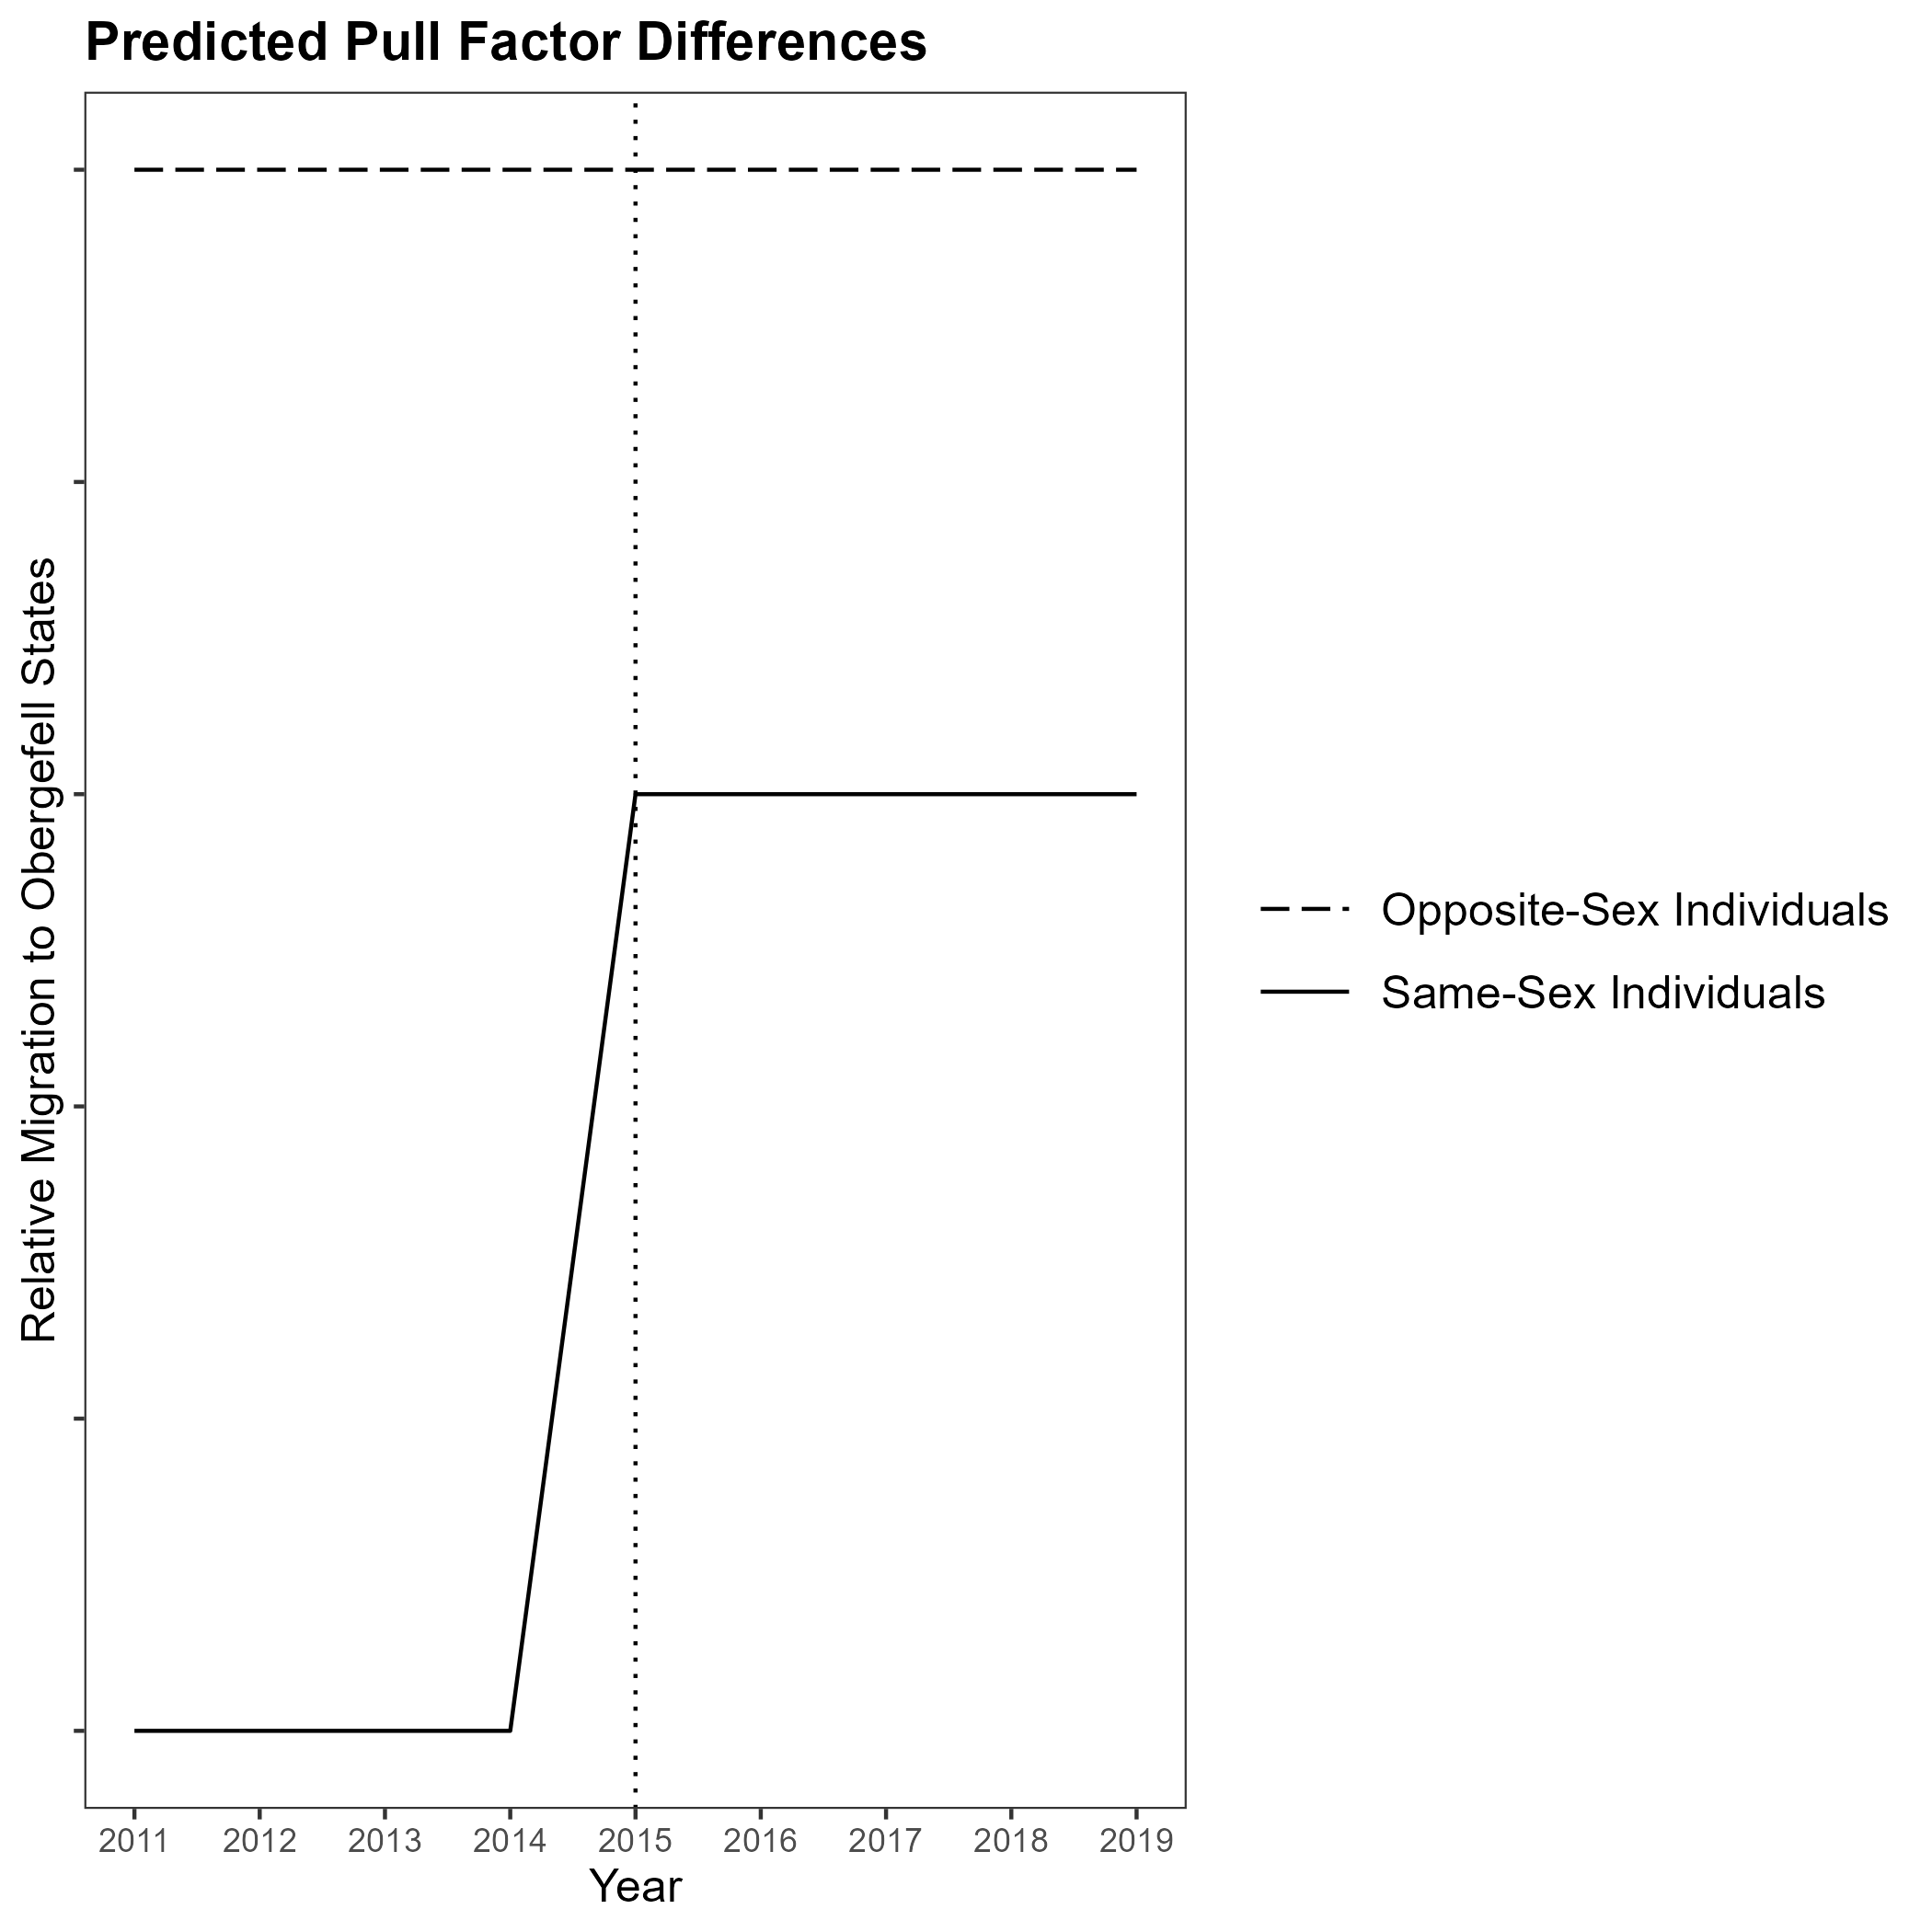
\includegraphics[width=0.75\linewidth]{outputs/summary_stats/ex_post_diffs.png}
    \caption{}
    \label{fig: ex_post_diffs}
\end{figure}

\begin{figure}
    \centering
    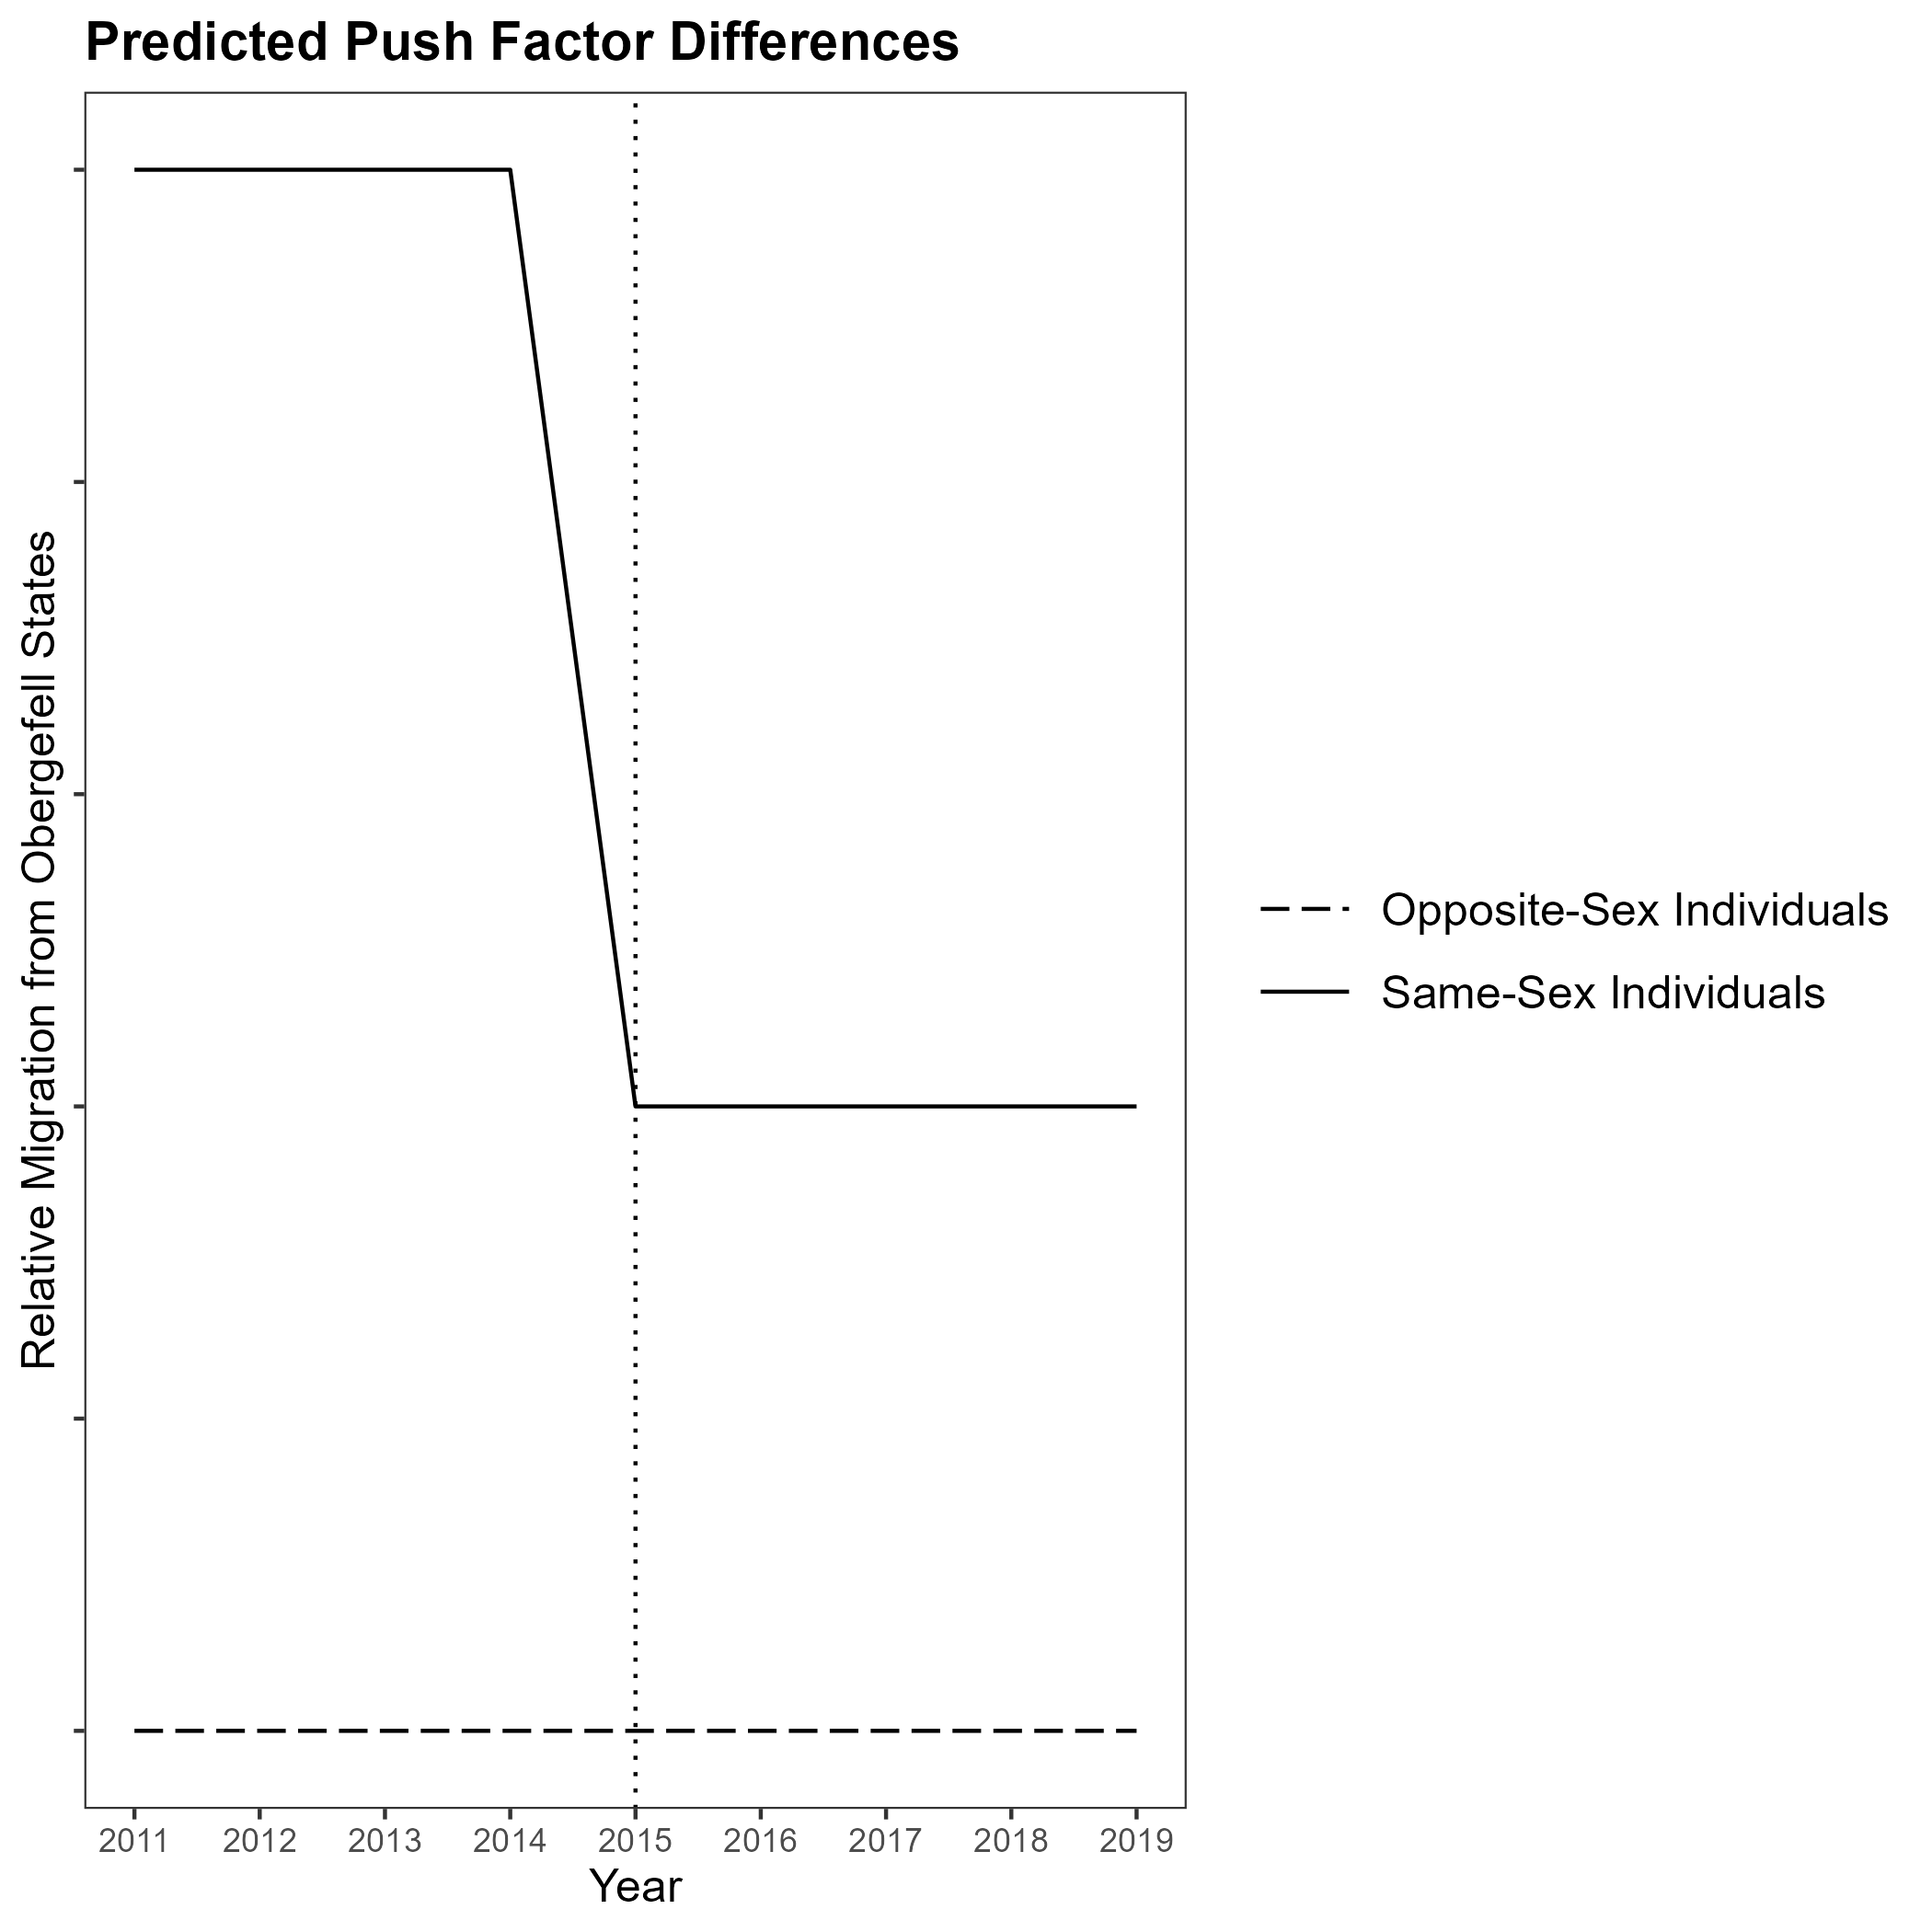
\includegraphics[width=0.75\linewidth]{outputs/summary_stats/ex_ante_diffs.png}
    \caption{}
    \label{fig: ex_ante_diffs}
\end{figure}
\end{centering}

\clearpage
\subsection{Main Model} %ok still need to fix centering
In table \ref{tab: expost_model} I present main regression results from “pull factor” models and in table \ref{tab: exante_model} I present main regression results from “push factor” models. In both tables, column 1 reports the regression coefficient of a model with only state and year fixed effects; column 2 reports the regression coefficient of a model with these fixed effects and controls for sex, race, education level, the presence of children in the household, income level, and age; and column 3 reports the regression coefficients of a model with these fixed effects, controls, and controls for an individual’s birth state. Figure \ref{fig: post_diffs} illustrates the underlying trends of the “pull factor” model while figure \ref{fig: ante_diffs} illustrates the underlying trends of the “push factor” model. 

Triple difference models require the assumption that there is an identifiable causal mechanism and that there are parallel trends \citep{24, 25}. In earlier sections, I have described plausible causal mechanisms. However, it can be seen in figure \ref{fig: post_diffs} and figure \ref{fig: ante_diffs} that the parallel trend assumption fails. There are a number of reasons for which this could occur. In the period between 2011 and 2015, there are significant changes in which states have “locally-legalized” same-sex marriage and which states do not. This means that one migrant identified as moving to (from) a “not-locally-legalized” state one year might have been identified as moving to (from) a “locally-legalized” state only one or two years later on. This could contribute to a violation of parallel trends as other factors, not related to same-sex marriage legalization but related to the sex of an individual’s partner, contribute to migration pattern differences across states. Further, the percentage of individuals migrating between states in any given year is relatively low, at (Z) percent. More noise is expected with smaller sample sizes. 

\begin{centering} %maybe just do centering in figures
\begin{figure}
    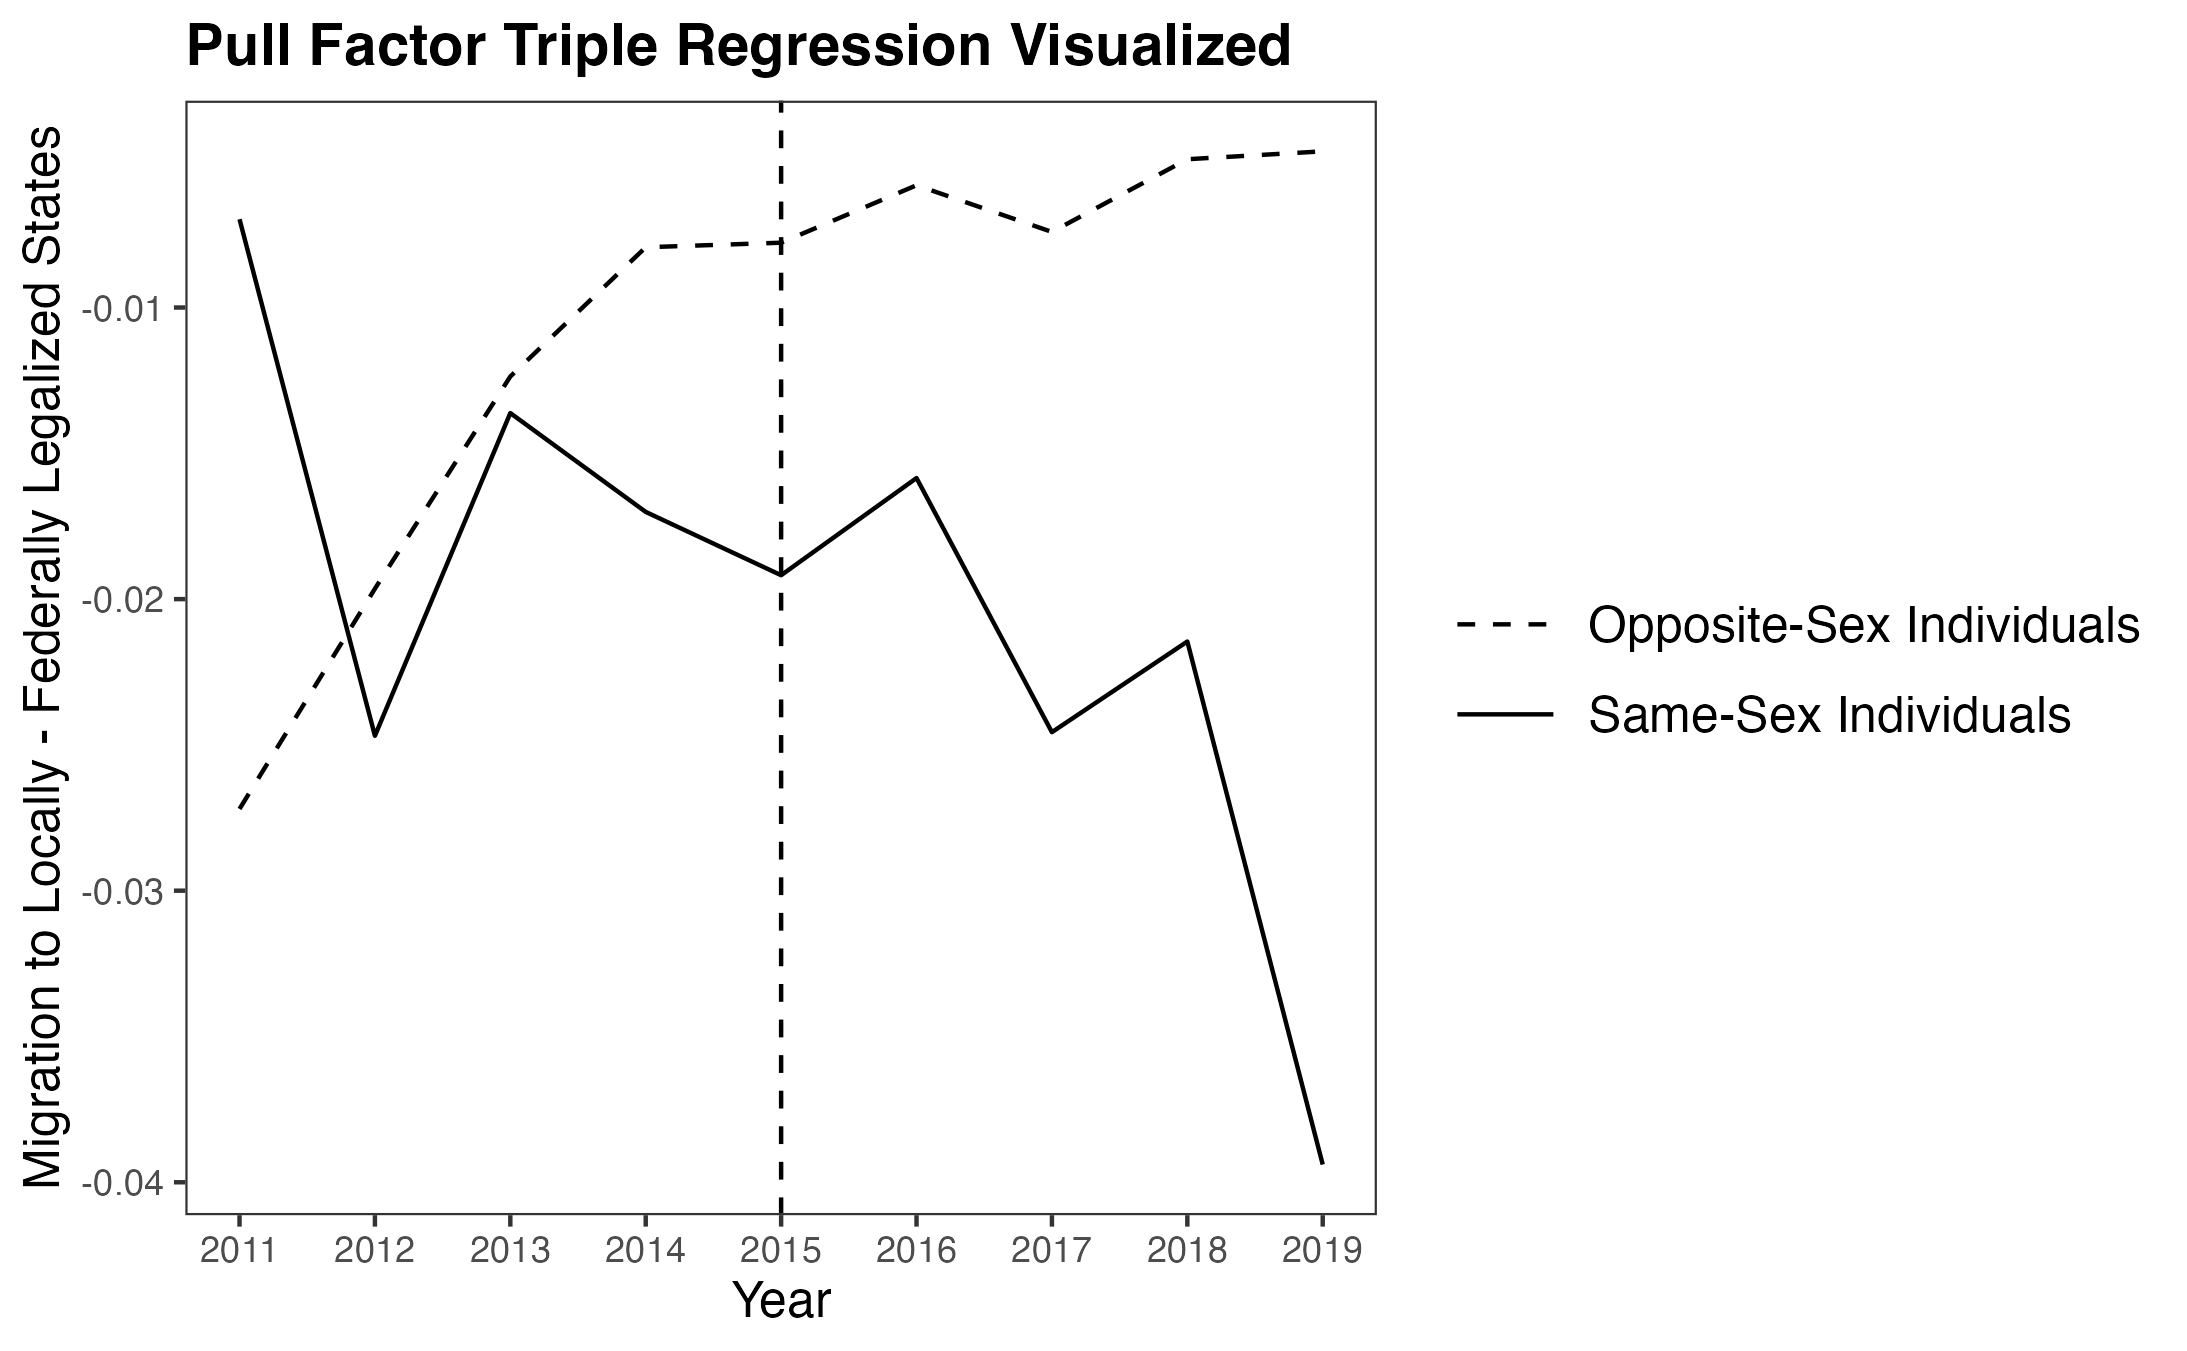
\includegraphics[width=0.75\linewidth]{outputs/summary_stats/post_diffs.png}
    \caption{}
    \label{fig: post_diffs}
\end{figure}

\begin{figure}
    \centering
    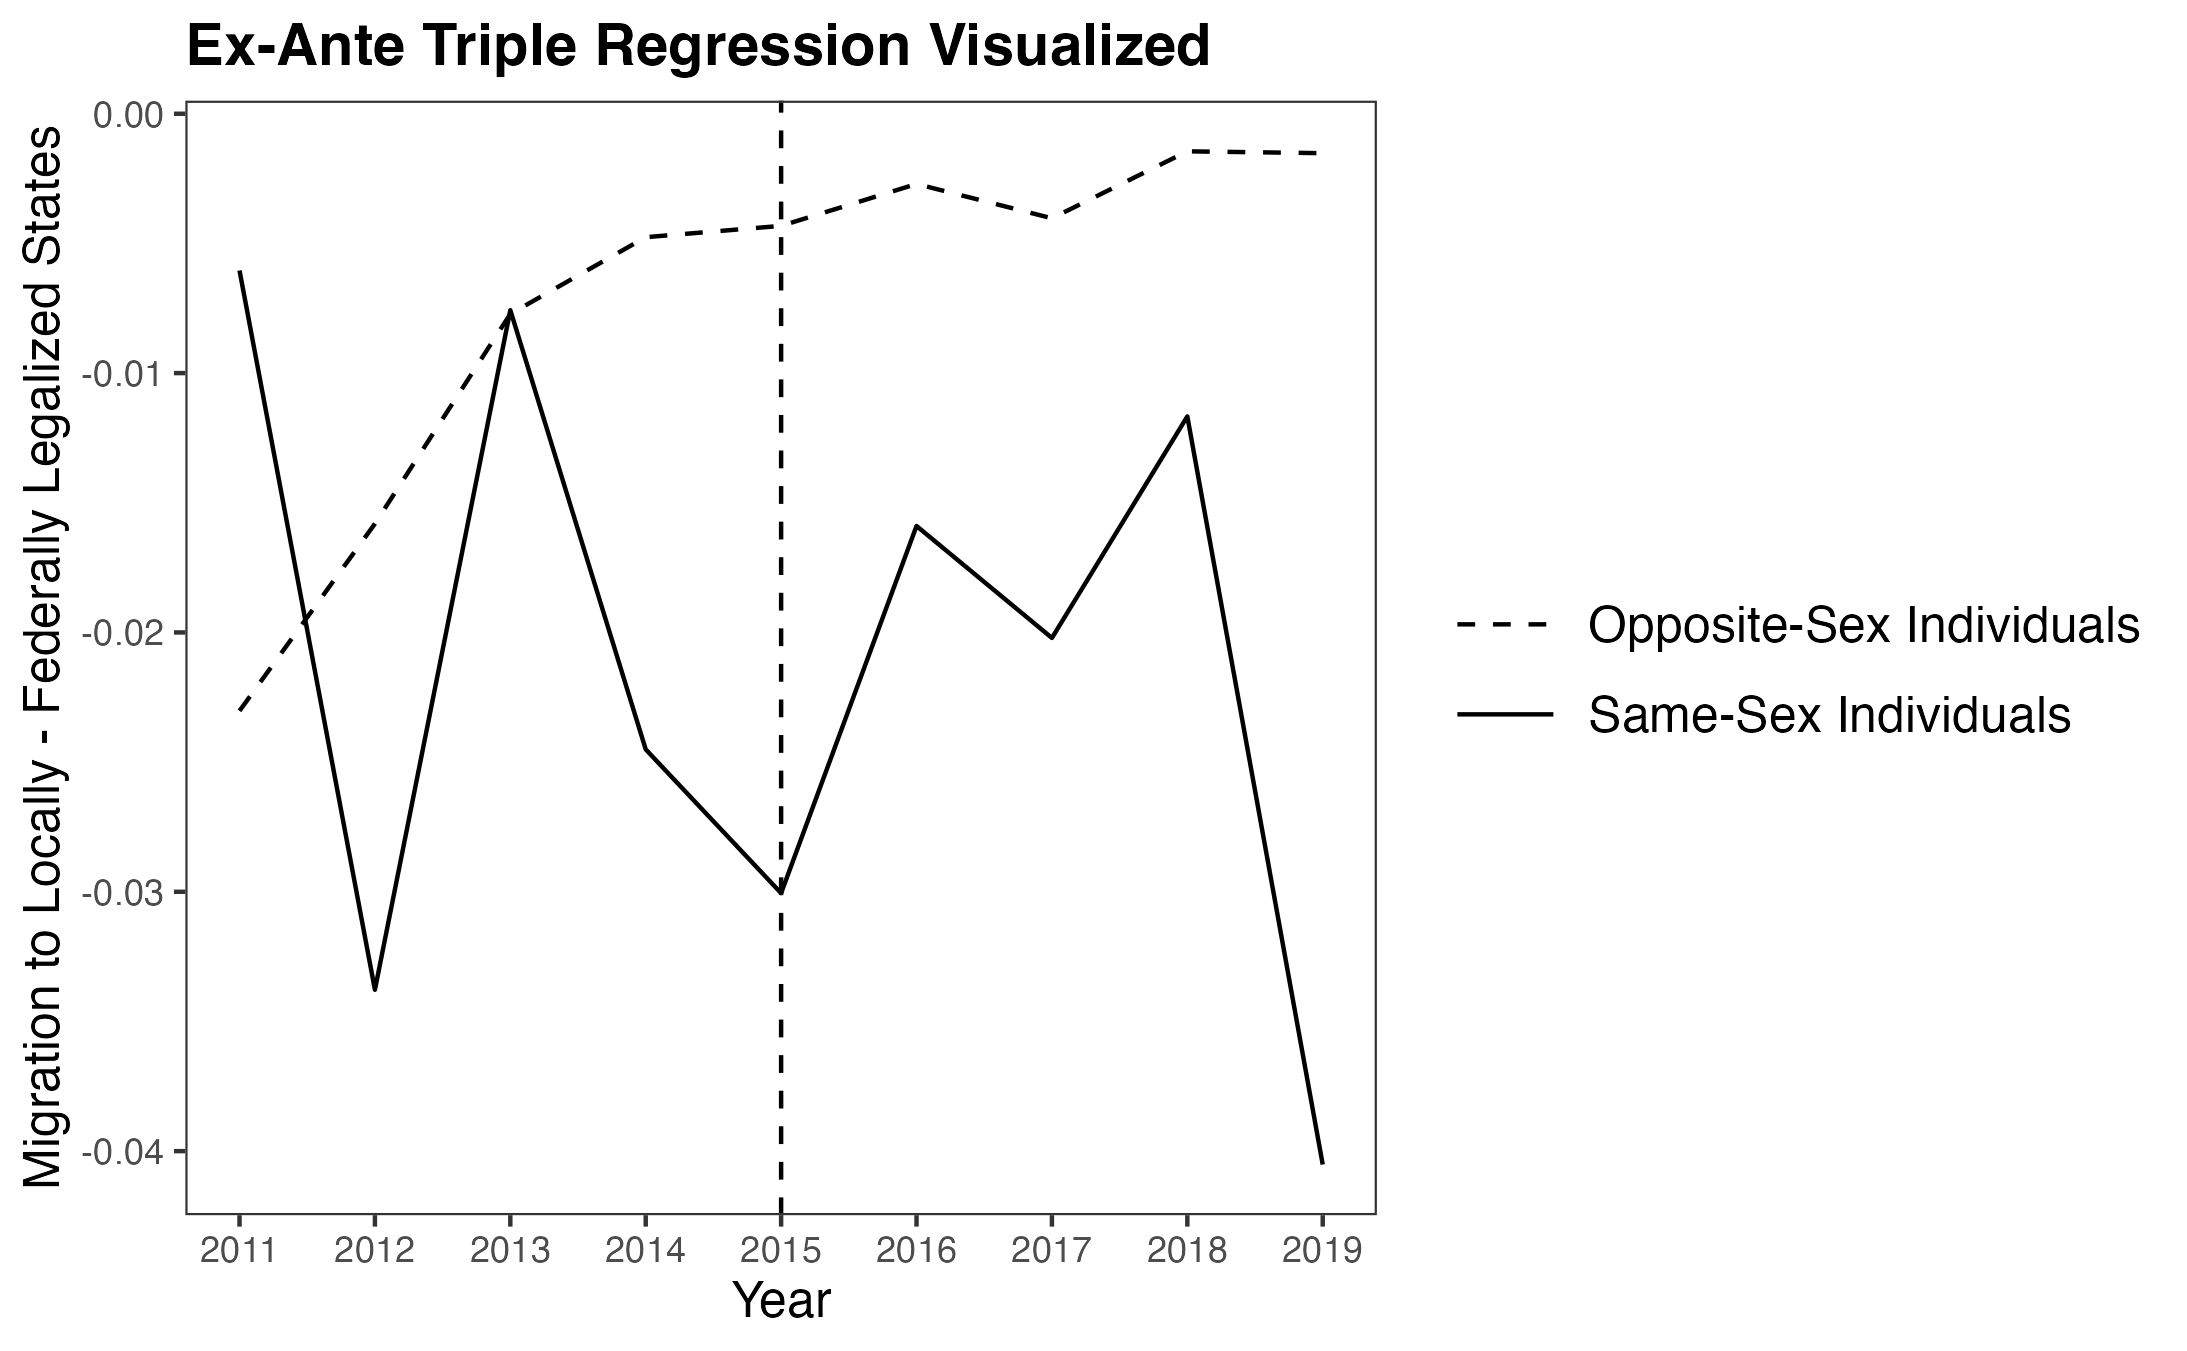
\includegraphics[width=0.75\linewidth]{outputs/summary_stats/ante_diffs.png}
    \caption{}
    \label{fig: ante_diffs}
\end{figure}
\end{centering}

In the “pull factor” model, the coefficient of interest is negative and statistically insignificant across all three models. Further, the standard error in models 2 and 3 suggests the true population mean could be 0 or positive. While the sign of the coefficients of interest is what I would expect, this means there is close to no difference between the fraction of same-sex individuals who moved to states that “locally-legalized” same-sex marriage and those that did not before and after 2015 relative to opposite-sex individuals. In other words, federal legalization led to minimal or no “pull factor” “dilution effect”. 

In the “push factor” model, the coefficient of interest is negative and statistically insignificant across all three models. Further, the standard error in all models suggests the true population mean could be 0 or positive. While the sign of the coefficients of interest is not what I would expect, this means there is close to no difference between the fraction of same-sex individuals who moved from states that “locally-legalized” same-sex marriage and those that did not before and after 2015 relative to opposite-sex individuals. In other words, federal legalization led to minimal or no “push factor” “dilution effect.”  

Even as both the “pull factor” and “push factor” model regressions similarly did not give support to my “dilution effect” hypothesis, they did so from directions opposite to which I predicted. This is puzzling: one model predicted slight decrease in migration to states that “locally-legalized” same-sex marriage after 2015; the other predicted a slight decrease in migration from states that “locally-legalized” same-sex marriage after 2015. This would suggest same-sex marriage was less of a “pull factor” but more of a “push factor” after 2015. One plausible explanation for this is related to sample size: the pool of migrants to a given state is larger than the pool of migrants from a given state. Using similar logic as above, it is less surprising that there is more deviation for the regressions run on smaller sample sizes. Other plausible explanations include that there is heterogeneity across states and individuals that obscure the effect of the “local-legalization” of same-sex marriage on the migration decisions of individuals in same-sex relationships, and that there are other, more salient factors, impacting the migration decisions of individuals in same-sex relationships. This heterogeneity and potential impact of other factors is explored in the following regressions. 

\begin{table}[h]
    \centering
    \begin{tabular}{lccc}
\multicolumn{4}{c}{Ex-Post Model} \\ \hline
 & (1) & (2) & (3) \\
VARIABLES & migrant & migrant & migrant \\ \hline
 &  &  &  \\
1.in\_samesex\#1.expost\_old\_legal\#1.post\_2015 & -0.015* & -0.013* & 0.013 \\
 & (0.007) & (0.006) & (0.033) \\
Constant & 0.106*** & 0.394*** & 3.356*** \\
 & (0.001) & (0.008) & (0.080) \\
 &  &  &  \\
Observations & 956,236,912 & 956,236,912 & 956,236,912 \\
 R-squared & 0.004 & 0.070 & 0.921 \\ \hline
\multicolumn{4}{c}{ Robust standard errors in parentheses} \\
\multicolumn{4}{c}{ *** p$<$0.01, ** p$<$0.05, * p$<$0.1} \\
\multicolumn{4}{c}{ Model 1 includes interaction terms and fixed effects only.} \\
\multicolumn{4}{c}{ )} \\
\multicolumn{4}{c}{ )} \\
\multicolumn{4}{c}{ )} \\
\multicolumn{4}{c}{ )} \\
\end{tabular}

    \caption{}
    \label{tab: expost_model}
\end{table}
\begin{table}[h]
    \centering
    \begin{tabular}{lccc}
\multicolumn{4}{c}{Ex-Ante Model} \\ \hline
 & (1) & (2) & (3) \\
VARIABLES & migrant & migrant & migrant \\ \hline
 &  &  &  \\
1.in\_samesex\#1.exante\_old\_legal\#1.post\_2015 & -0.016 & -0.014 & 0.014 \\
 & (0.009) & (0.008) & (0.030) \\
Constant & 0.106*** & 0.394*** & 3.757*** \\
 & (0.001) & (0.007) & (0.123) \\
 &  &  &  \\
Observations & 956,236,912 & 956,236,912 & 956,236,912 \\
 R-squared & 0.003 & 0.069 & 0.912 \\ \hline
\multicolumn{4}{c}{ Robust standard errors in parentheses} \\
\multicolumn{4}{c}{ *** p$<$0.01, ** p$<$0.05, * p$<$0.1} \\
\multicolumn{4}{c}{p{\textwidth}}{ Model 1 includes interaction terms and fixed effects only. \newline
Model 2 includes interaction terms, fixed effects, and controls for sex, race, education, age, and income. \newline
Model 3 includes interaction terms, fixed effects, and controls for sex, race, education, age, income, and birthstate. \newline
Models 1 and 2 use a weighted sample. Model 3 uses a weighted and collapsed sample.} \\
\multicolumn{4}{c}{ )} \\
\multicolumn{4}{c}{ )} \\
\multicolumn{4}{c}{ )} \\
\multicolumn{4}{c}{ )} \\
\end{tabular}

    \caption{}
    \label{tab: exante_model}
\end{table}

\clearpage
\subsection{Flow Heterogeneity}

One source of heterogeneity is from which type of state an individual might move in the “pull factor” model and to which type of state an individual might move in the “push factor” model. If fewer individuals in same-sex relationships move between “locally-legalized” states after 2015, that could make the “push factor” model coefficient negative even if more individuals in same-sex relationships move from “locally-legalized” to “not-locally-legalized” states after 2015. This could help explain the opposite-than-expected main “push factor” regression results.

Table \ref{tab: flow_expost_model} presents regression results from “pull factor” models in which the outcome variable indicates whether an individual migrated from a state with “locally-legalized” same-sex marriage, migrated from a state that had “not-locally-legalized” same-sex marriage, or whether an individual did not migrate from a different state. Table \ref{tab: flow_exante_model} presents regression results from “push factor” models in which the outcome variable indicates whether an individual migrated to a state with “locally-legalized” same-sex marriage, migrated to a state that had “not-locally-legalized” same-sex marriage, or whether an individual did not migrate to a different state. M1, M2, and M3 refer to the varying levels of controls that differentiated columns 1, 2, and 3 in the main model regressions.  Figure \ref{fig: flows_post_diffs} illustrates the underlying trends of the “pull factor” model while figure \ref{fig: flows_ante_diffs} illustrates the underlying trends of the “push factor” model with the modified outcome variables.

As these regressions are still triple difference models, assumptions of a plausible causal mechanism and parallel trends are still needed \citep{24, 25}. In line with the “dilution effect”, I would expect there to be slightly less migration between states that “locally legalized” same-sex marriage after 2015, as previously “not-locally-legalized” states become marginally more attractive for those in same-sex relationships. On the other hand, I would expect there to be more migration from states that “locally-legalized” same-sex marriage to states that had “not-locally-legalized” same-sex marriage after 2015, and less migration from states that had “not-locally-legalized” same-sex marriage to states that “locally-legalized” same-sex marriage after 2015. Figures \ref{fig: flows_post_diffs} and \ref{fig: flows_ante_diffs} illustrate that parallel trends do not hold for any of the modified outcome variables. However, it is important to note that the to (from) “not-locally-legalized” trends appear significantly less noisy.

\begin{centering}
\begin{figure}
    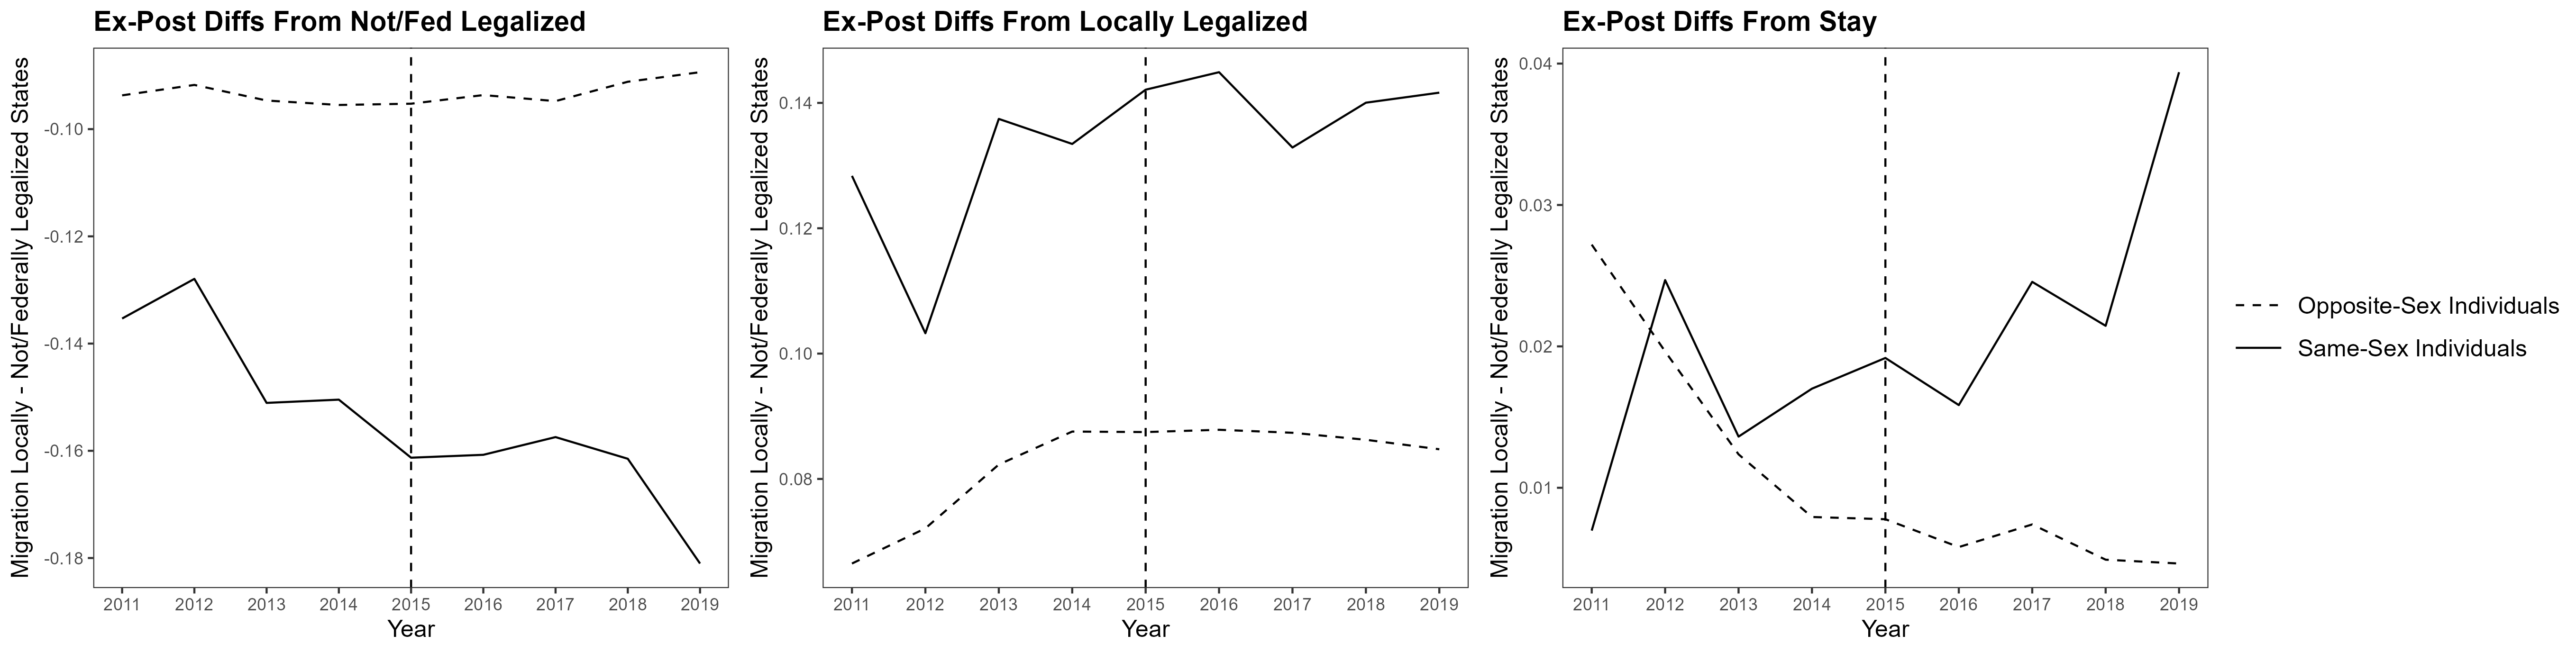
\includegraphics[width=1\linewidth]{outputs/summary_stats/flows_post_diffs.png}
    \caption{}
    \label{fig: flows_post_diffs}
\end{figure}

\begin{figure}
    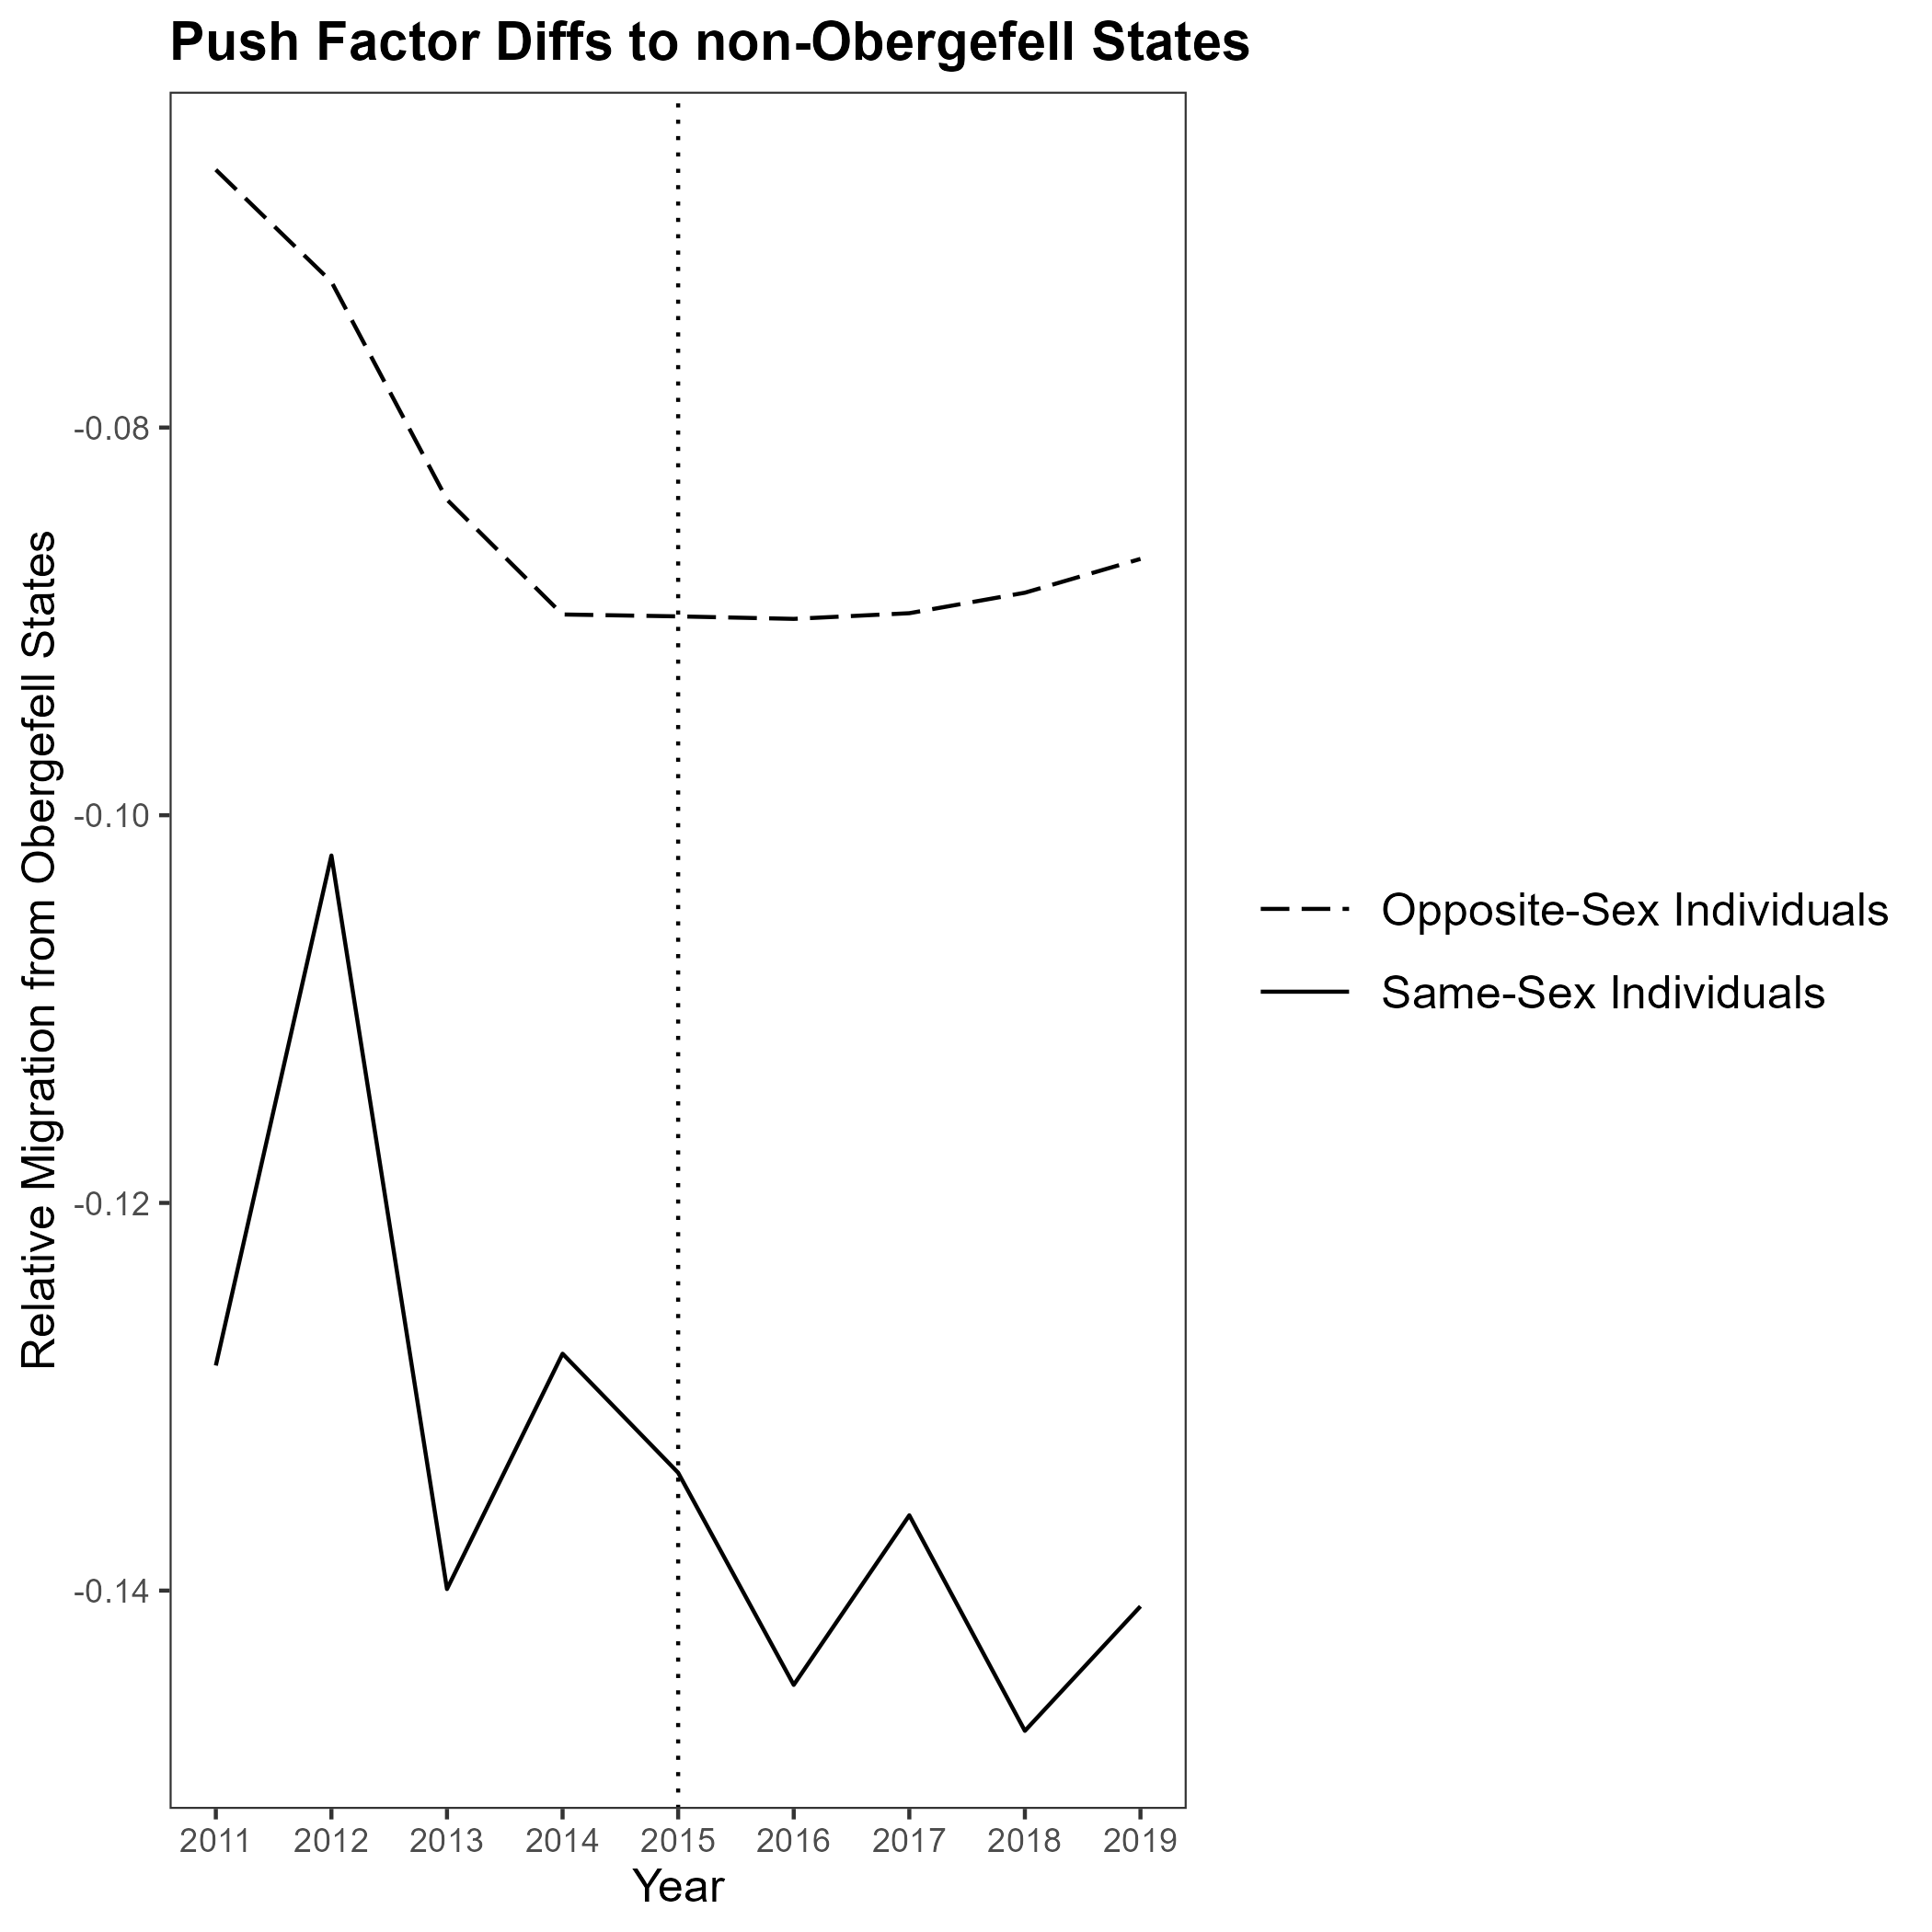
\includegraphics[width=1\linewidth]{outputs/summary_stats/flows_ante_diffs.png}
    \caption{}
    \label{fig: flows_ante_diffs}
\end{figure}
\end{centering}

 The two coefficients of interest in this exercise are those in columns (7) and (8) of table \ref{tab: flow_exante_model}. The coefficient in column (7) is negative and statistically insignificant and the coefficient in column (8) is positive and statistically insignificant. The standard error in both columns suggests the true population mean could be 0 or of the opposite sign. This indicates that those in same-sex relationships were slightly less likely to move from “locally-legalized” states to “not-locally-legalized” states and slightly more likely to move to other “locally-legalized” states. This is the opposite of what I would have predicted under my theory. This then suggests that flow heterogeneity, as measured, does not contribute to the opposite-than-expected results in the main “push factor” regression.


\begin{landscape}
\begin{scriptsize}
\begin{table}[h] %maybe put on top
    \centering
    \begin{tabular}{lccccccccc} \hline
 & (1) & (2) & (3) & (4) & (5) & (6) & (7) & (8) & (9) \\
VARIABLES & M1: From Fed/Not & M1: From Local & M1: Stay & M2: From Fed/Not & M2: From Local & M2: Stay & M3: From Fed/Not & M3: From Local & M3: Stay \\ \hline
 &  &  &  &  &  &  &  &  &  \\
post\_treatment & -0.035*** & 0.025** & 0.010 & -0.016 & 0.015 & 0.001 & -0.005 & 0.004 & 0.002 \\
 & (0.010) & (0.011) & (0.008) & (0.029) & (0.023) & (0.026) & (0.034) & (0.030) & (0.030) \\
Constant & 0.103*** & 0.000*** & 0.897*** & 1.968*** & 2.095*** & -3.063*** & 1.812*** & 2.102*** & -2.913*** \\
 & (0.000) & (0.000) & (0.000) & (0.325) & (0.350) & (0.131) & (0.342) & (0.352) & (0.108) \\
 &  &  &  &  &  &  &  &  &  \\
Observations & 19,755 & 19,755 & 19,755 & 19,755 & 19,755 & 19,755 & 19,755 & 19,755 & 19,755 \\
 R-squared & 0.047 & 0.046 & 0.005 & 0.531 & 0.511 & 0.922 & 0.557 & 0.548 & 0.927 \\ \hline
\multicolumn{10}{c}{ Robust standard errors in parentheses} \\
\multicolumn{10}{c}{ *** p$<$0.01, ** p$<$0.05, * p$<$0.1} \\
\multicolumn{10}{c}{ See below.} \\
\end{tabular}

    \caption{}
    \label{tab: flow_expost_model}
\end{table}
\begin{table}[h]
    \centering
    \begin{tabular}{lccccccccc} \hline
 & (1) & (2) & (3) & (4) & (5) & (6) & (7) & (8) & (9) \\
VARIABLES & M1: To Fed/Not & M1: To Local & M1: Stay & M2: To Fed/Not & M2: To Local & M2: Stay & M3: To Fed/Not & M3: To Local & M3: Stay \\ \hline
 &  &  &  &  &  &  &  &  &  \\
ante\_treatment & -0.031*** & 0.023* & 0.008 & -0.011 & 0.011 & -0.000 & 0.001 & 0.002 & -0.003 \\
 & (0.008) & (0.011) & (0.012) & (0.024) & (0.022) & (0.024) & (0.027) & (0.029) & (0.025) \\
Constant & 0.181*** & 0.005*** & 0.814*** & 0.288 & 3.639*** & -2.927*** & 0.498 & 3.561*** & -3.059*** \\
 & (0.000) & (0.000) & (0.000) & (0.822) & (0.802) & (0.189) & (0.926) & (0.874) & (0.226) \\
 &  &  &  &  &  &  &  &  &  \\
Observations & 956,236,912 & 956,236,912 & 956,236,912 & 956,236,912 & 956,236,912 & 956,236,912 & 956,236,912 & 956,236,912 & 956,236,912 \\
 R-squared & 0.047 & 0.045 & 0.004 & 0.494 & 0.533 & 0.919 & 0.527 & 0.559 & 0.921 \\ \hline
\multicolumn{10}{c}{ Robust standard errors in parentheses} \\
\multicolumn{10}{c}{ *** p$<$0.01, ** p$<$0.05, * p$<$0.1} \\
\multicolumn{10}{c}{ See below.} \\
\end{tabular}

    \caption{}
    \label{tab: flow_exante_model}
\end{table}
\end{scriptsize}
\end{landscape}

%\subsection{State Comparisons- ie something like CA v TX}

\clearpage
\subsection{Gender Heterogeneity}

Another source of heterogeneity is an individual’s gender. If same-sex marriage legalization affects the behavior of men in same-sex relationships differently than women, that could impact the main regression results.

Table \ref{tab: sex_expost_model} presents regression results from “pull factor” models split by gender. Table \ref{tab: sex_exante_model} presents regression results from “push factor” models split by gender. Model 1, Model 2, and Model 3 refer to the varying levels of controls that differentiated columns 1, 2, and 3 in the main model regressions.  Figure \ref{fig: sex_post_diffs} illustrates the underlying trends of the “pull factor” model while figure \ref{fig: sex_ante_diffs} illustrates the underlying trends of the “push factor” model by region.

As these regressions are still triple difference models, assumptions of a plausible causal mechanism and parallel trends are still needed \citep{24, 25}. Like in the main model, plausible causal mechanisms are explained in earlier sections. However, it is important to note that research by \citet{1, 12} indicates same-sex marriage legalization could lead to larger behavioral changes for men in same-sex relationship. Figures \ref{fig: sex_post_diffs} and \ref{fig: sex_ante_diffs} illustrate that parallel trends hold for men but not women. Indeed, the “pull factor” figure for men roughly corresponds with what I predicted.

\begin{centering}
\begin{figure}
    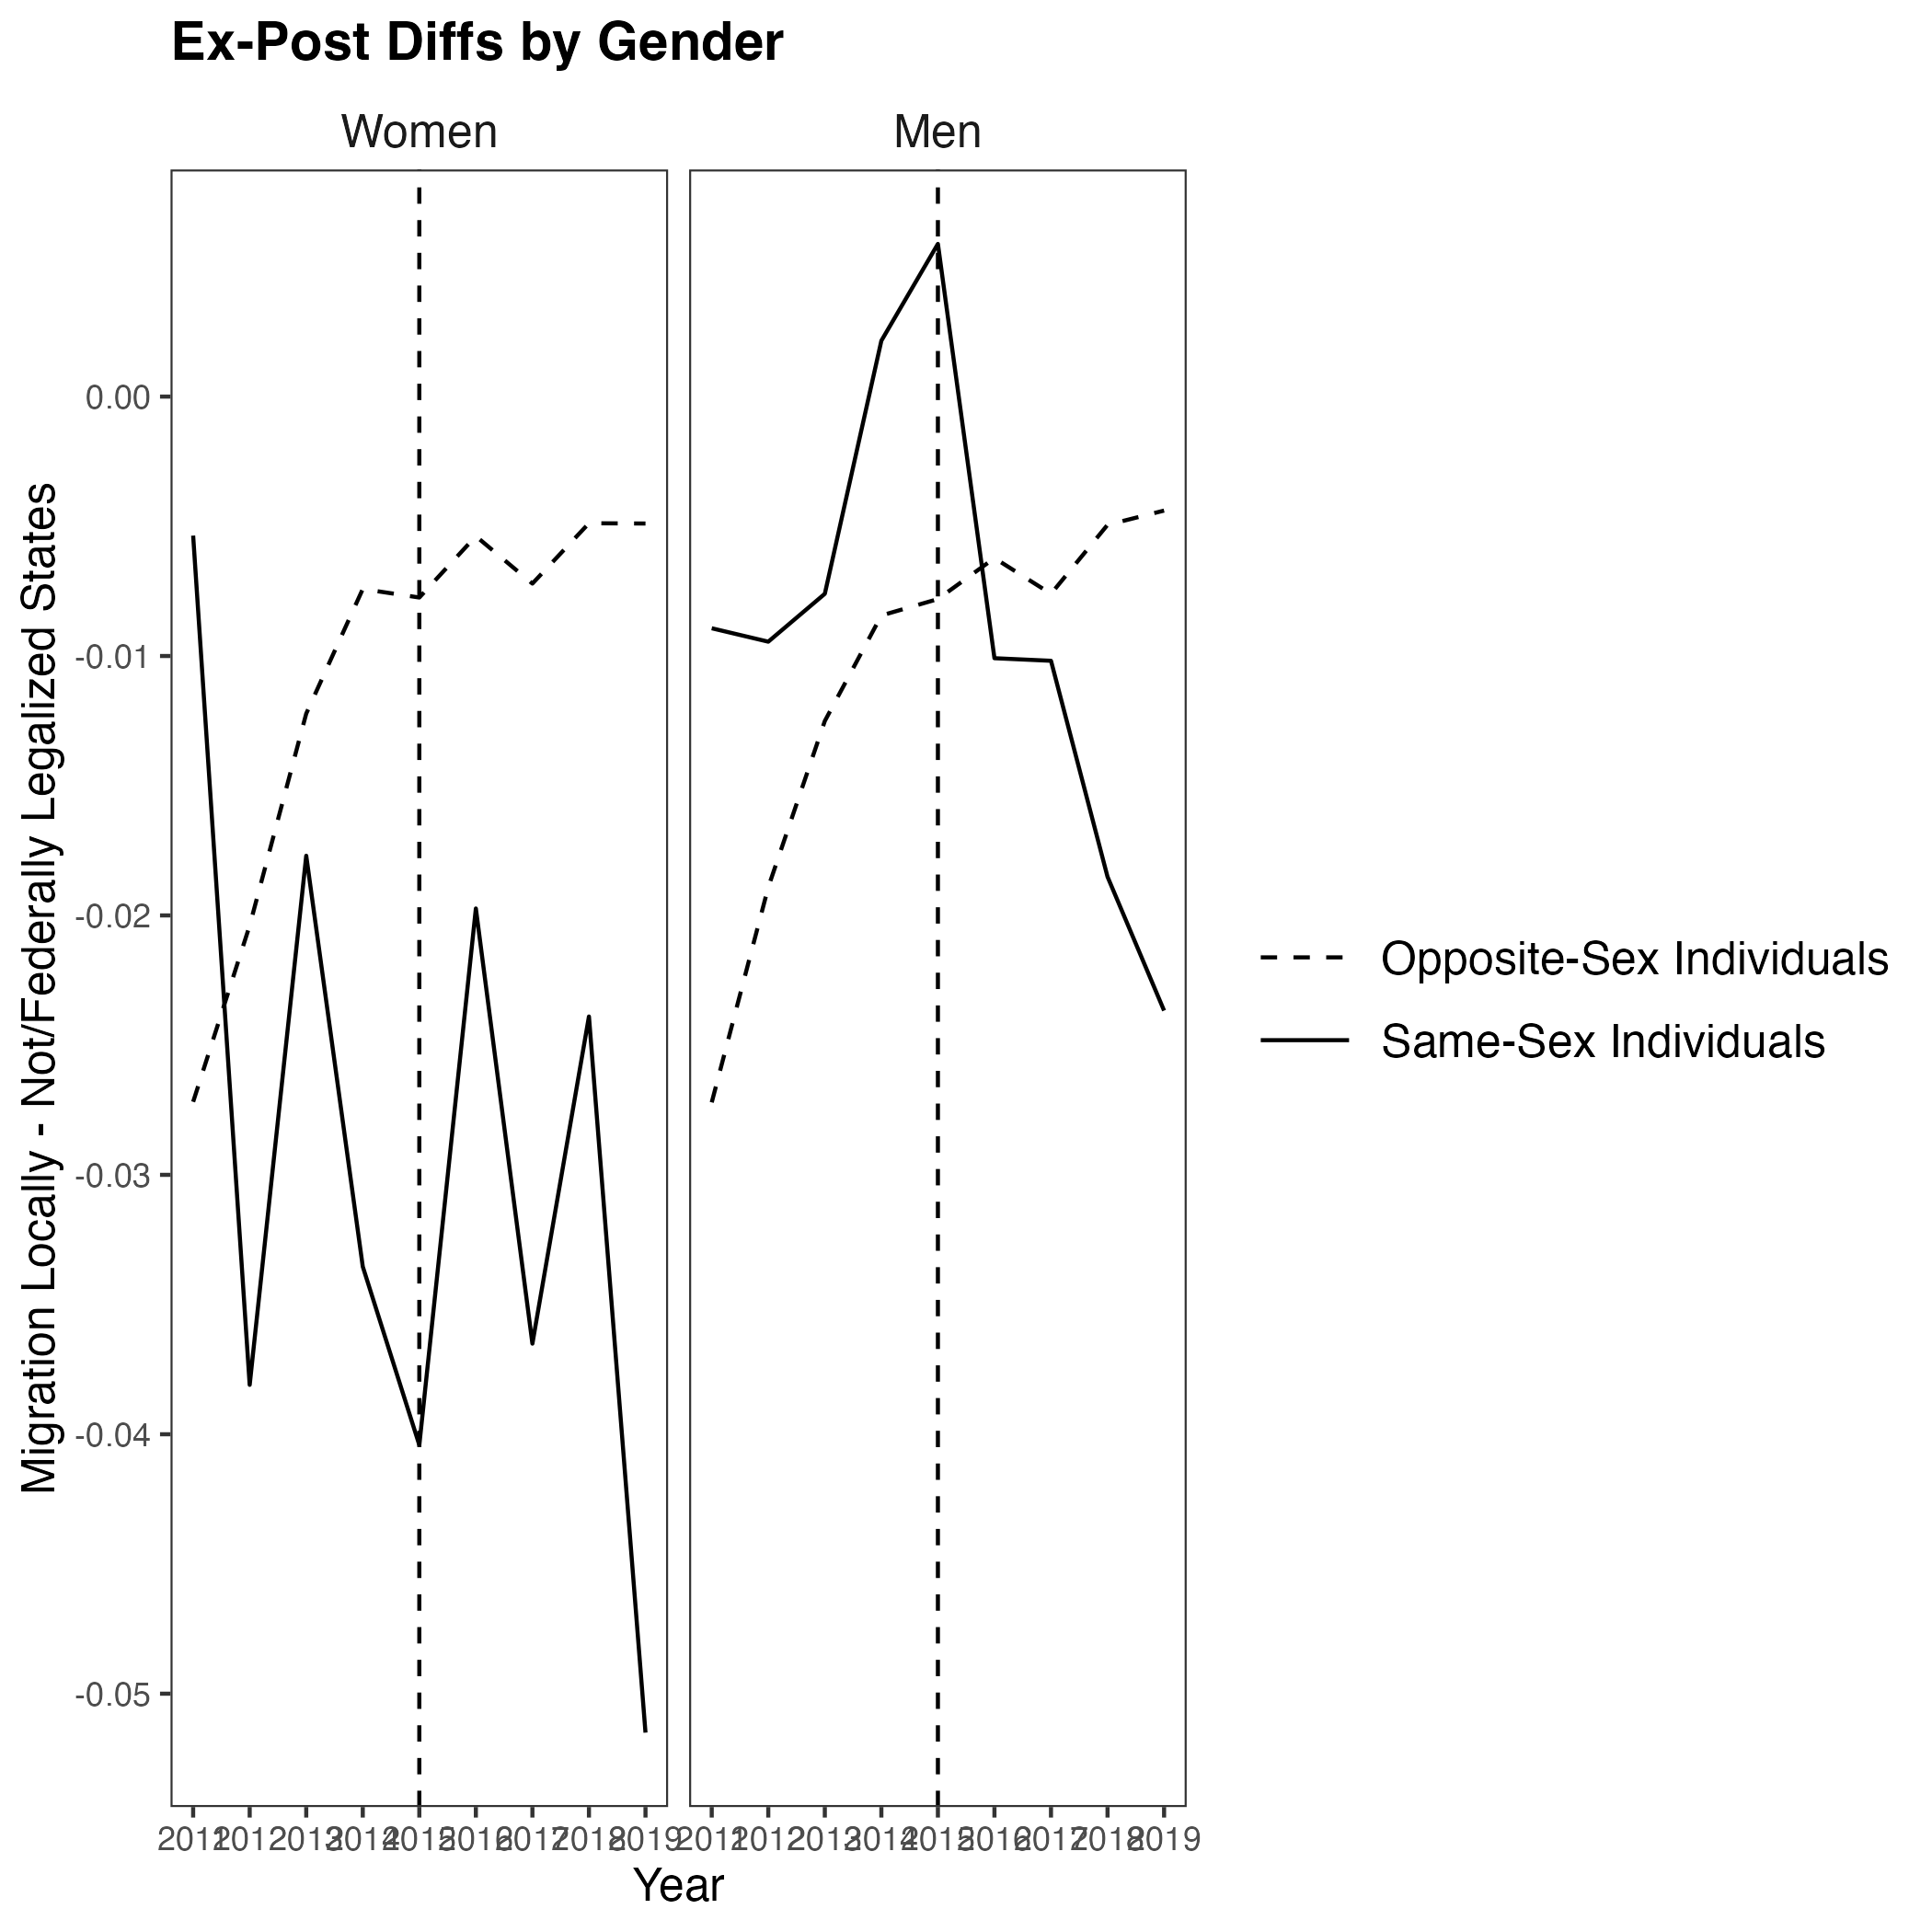
\includegraphics[width=1\linewidth]{outputs/summary_stats/sex_post_diffs.png}
    \caption{}
    \label{fig: sex_post_diffs}
\end{figure}

\begin{figure}
    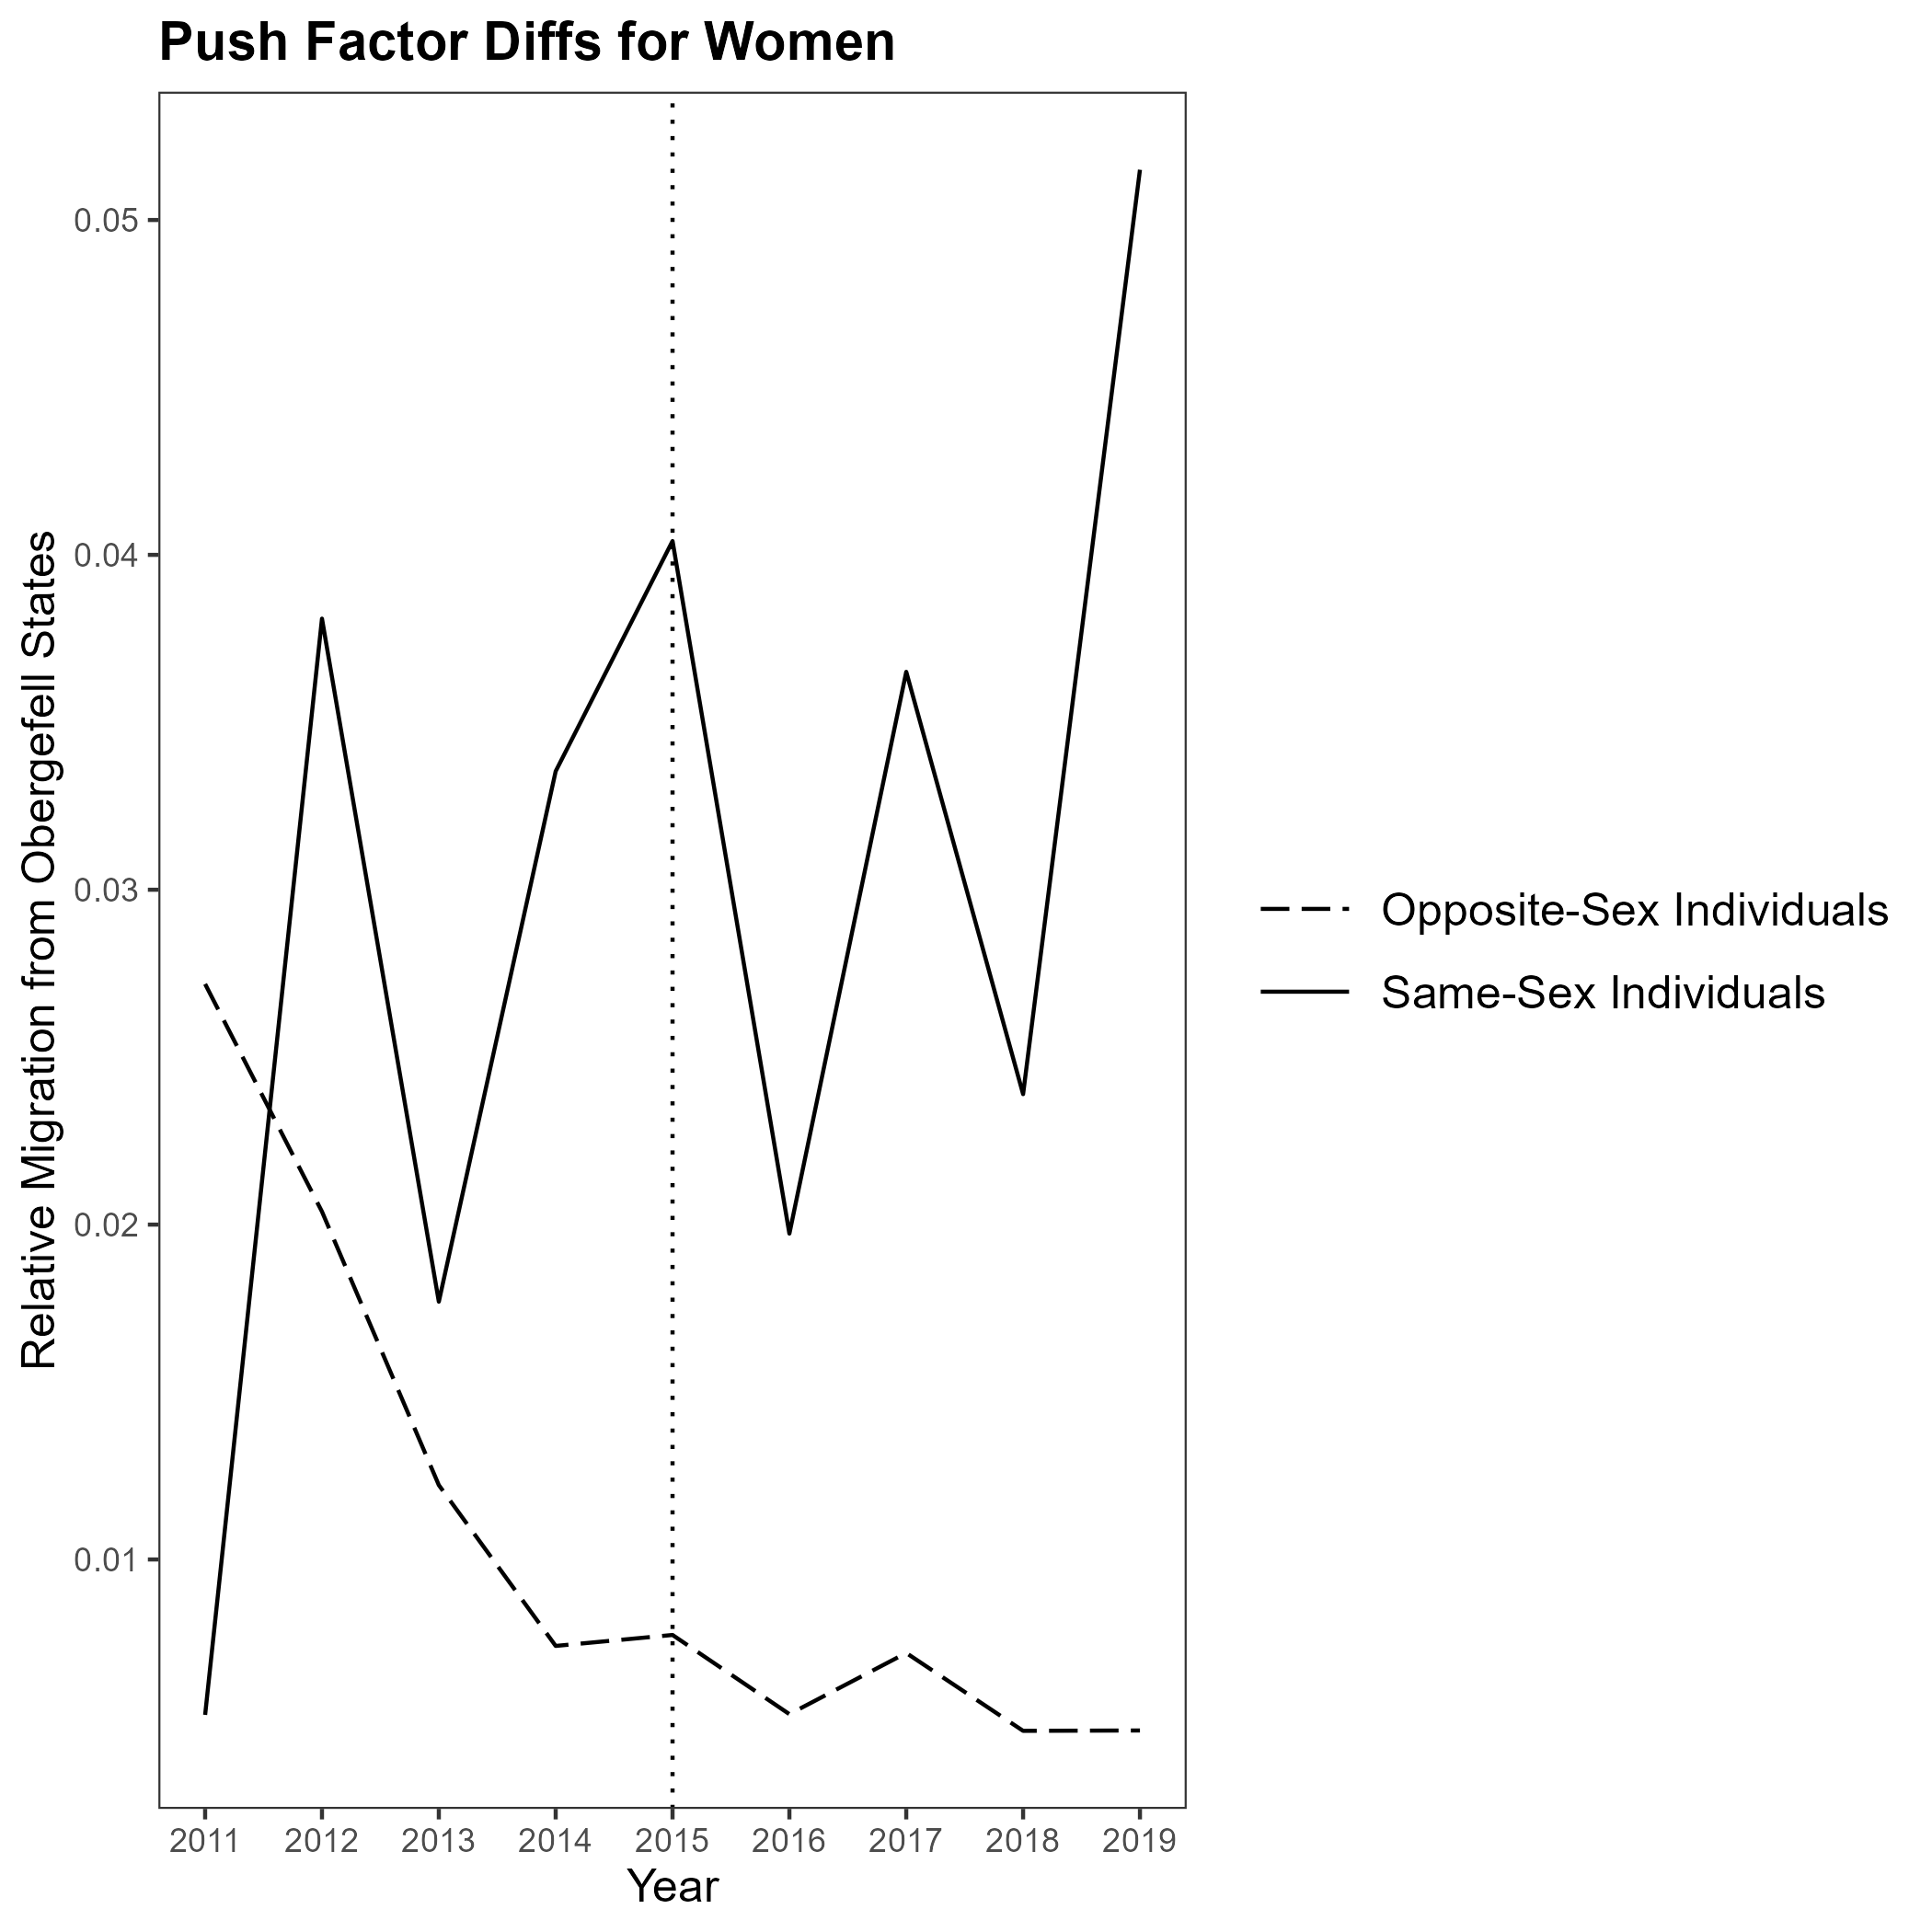
\includegraphics[width=1\linewidth]{outputs/summary_stats/sex_ante_diffs.png}
    \caption{}
    \label{fig: sex_ante_diffs}
\end{figure}
\end{centering}

The two coefficients of interest in this exercise are those in columns (5) and (6). While it is interesting that the coefficients for men and women have opposite signs, even as they are all statistically insignificant, this does not provide greater insight why the main “push” model coefficients are negative. This then suggests that gender heterogeneity, as measured, does not contribute to the opposite-than-expected results in the main “push factor” regression.


\begin{scriptsize}
\begin{table}[h]
    \centering
    \begin{tabular}{lc}
\multicolumn{2}{c}{Ex-Post Model by Sex} \\ \hline
 & (1) \\
VARIABLES & Model 1: Men \\ \hline
 &  \\
1.in\_samesex\#1.expost\_old\_legal\#1.post\_2015 & -0.005*** \\
 & (0.001) \\
Constant & 0.106*** \\
 & (0.001) \\
 &  \\
Observations & 481,915,892 \\
 R-squared & 0.004 \\ \hline
\multicolumn{2}{c}{ Robust standard errors in parentheses} \\
\multicolumn{2}{c}{ *** p$<$0.01, ** p$<$0.05, * p$<$0.1} \\
\multicolumn{2}{c}{ See below.} \\
\end{tabular}

    \caption{}
    \label{tab: sex_expost_model}
\end{table}
\begin{table}[h]
    \centering
    \begin{tabular}{lcc}
\multicolumn{3}{c}{Ex-Ante Model} \\ \hline
 & (1) & (2) \\
VARIABLES & Model 1: Male & Model 1: Female \\ \hline
 &  &  \\
ante\_treatment & -0.005 & -0.010 \\
 & (0.010) & (0.013) \\
Constant & 0.185*** & 0.186*** \\
 & (0.000) & (0.000) \\
 &  &  \\
Observations & 481,915,892 & 474,321,020 \\
 R-squared & 0.004 & 0.004 \\ \hline
\multicolumn{3}{c}{ Robust standard errors in parentheses} \\
\multicolumn{3}{c}{ *** p$<$0.01, ** p$<$0.05, * p$<$0.1} \\
\multicolumn{3}{c}{ See below.} \\
\end{tabular}

    \caption{}
    \label{tab: sex_exante_model}
\end{table}
\end{scriptsize}

\clearpage
\subsection{Region Heterogeneity}

Another source of heterogeneity is from which region an individual comes from in the “push factor” model and to which region an individual is in the “pull factor” model. While the main model includes state-level fixed effects, it does not directly control for distance between states. \citep{1} suggests distance impacts what type of state an individual moves to (from), as individuals are less likely to move to states further away. If an individual’s region has relatively more “locally legalized” states, that could make the  “push factor” coefficient less positive as “not locally legalized” states are relatively further away. If an individual’s region has both “locally legalized” and “not locally legalized” states, coefficients of interest should be as predicted in line with the “dilution effect”. This could help explain the opposite-than-expected main “push factor” regression results.

Table \ref{tab: region_expost_model} presents regression results from “pull factor” models split by region. Table \ref{tab: region_exante_model} presents regression results from “push factor” models split by region. Model 1, Model 2, and Model 3 refer to the varying levels of controls that differentiated columns 1, 2, and 3 in the main model regressions.  Figure \ref{fig: region_post_diffs} illustrates the underlying trends of the “pull factor” model while figure \ref{fig: region_ante_diffs} illustrates the underlying trends of the “push factor” model by region. The northeast and west “push factor” figures are cut off after 2013 as all states in the northeast and west locally legalized same-sex marriage by 2014.

As these regressions are still triple difference models, assumptions of a plausible causal mechanism and parallel trends are still needed \citep{24, 25}. Like in the main model, plausible causal mechanisms are explained in earlier sections, albeit with further elaboration in the first paragraph of this subsection. Figures \ref{fig: region_post_diffs} and \ref{fig: region_ante_diffs} illustrate that parallel trends roughly hold for the midwest and south “pull factor” models and for all “push factor” models. 

\begin{centering}
\begin{figure}
    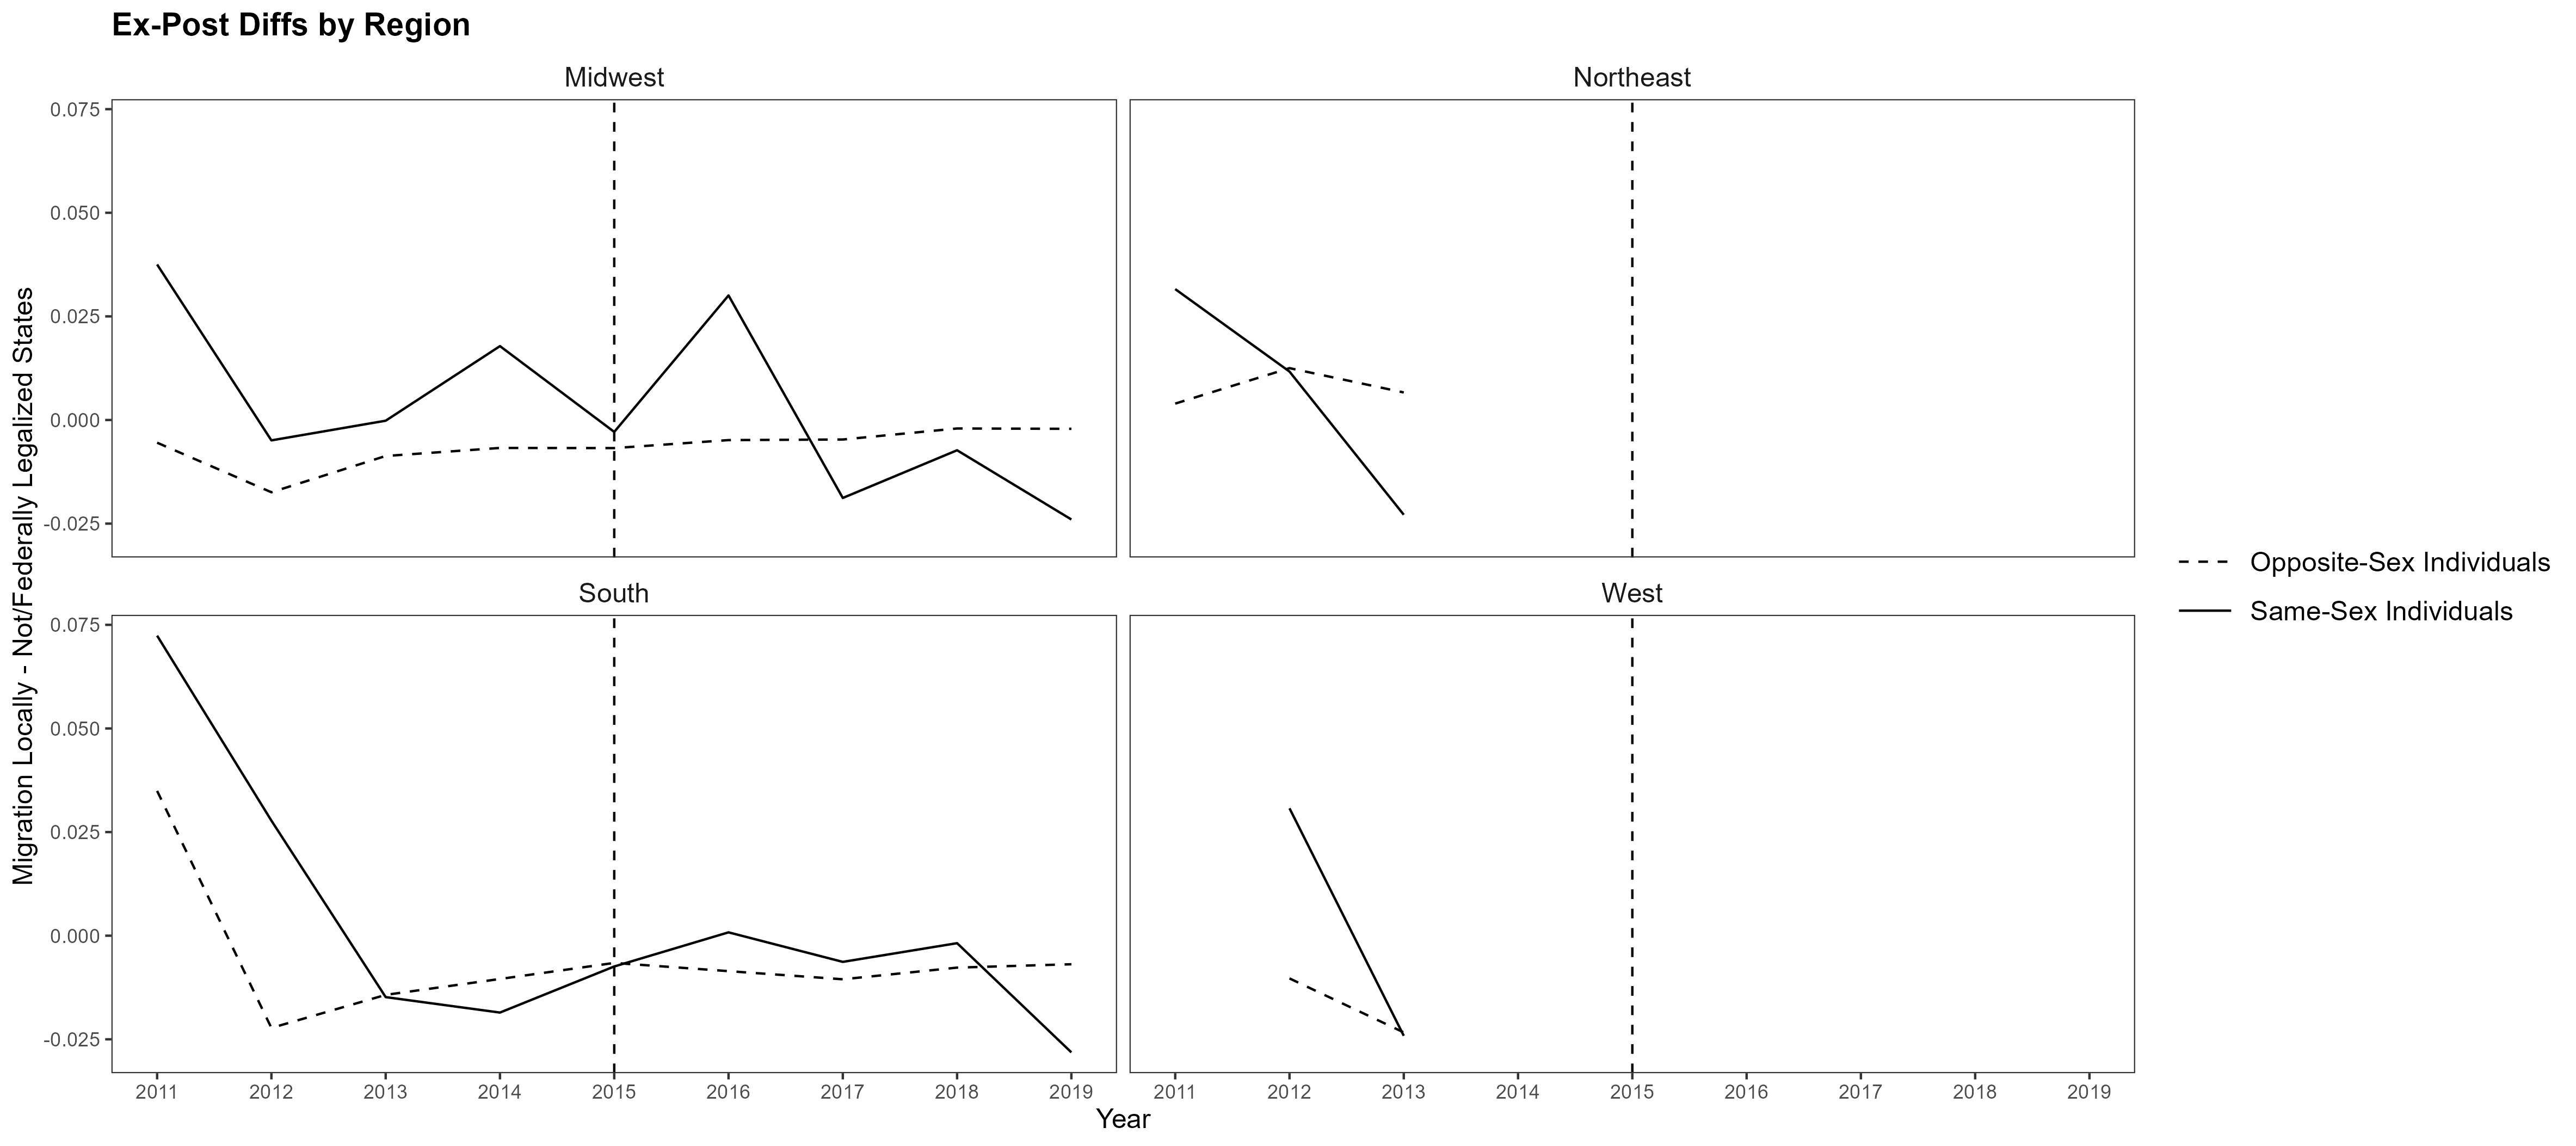
\includegraphics[width=1\linewidth]{outputs/summary_stats/region_post_diffs.png}
    \caption{}
    \label{fig: region_post_diffs}
\end{figure}

\begin{figure}
    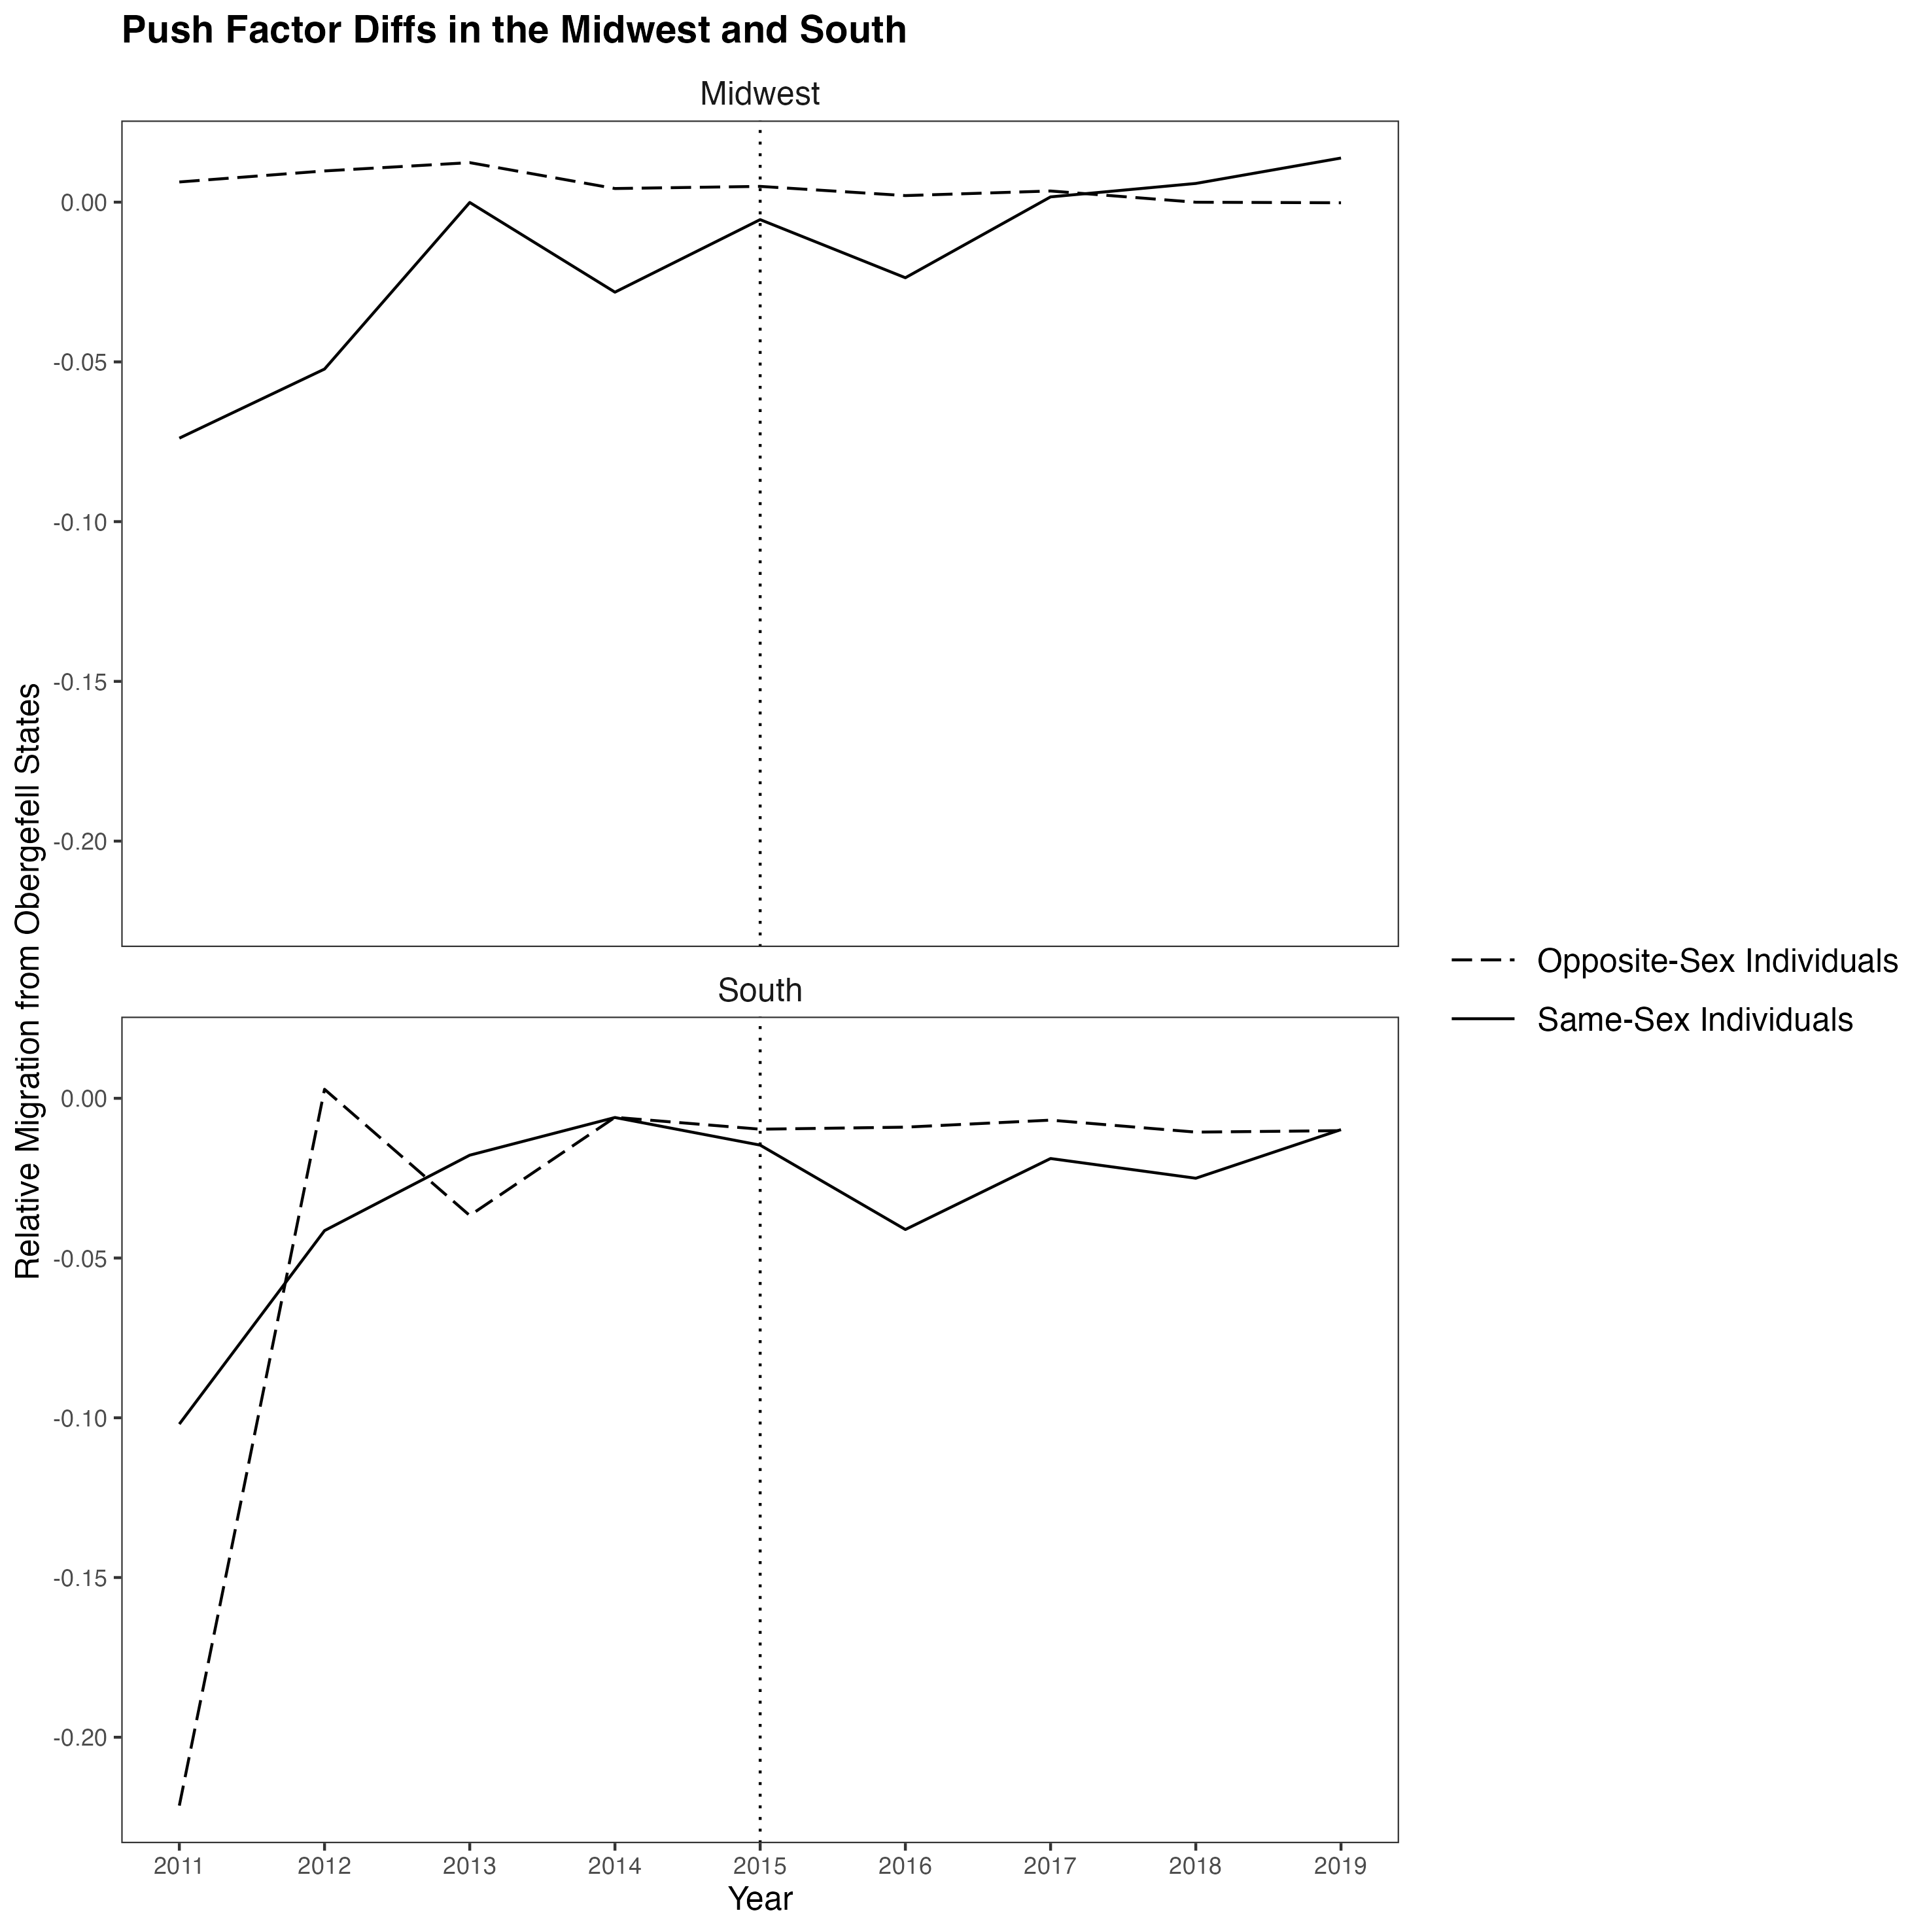
\includegraphics[width=1\linewidth]{outputs/summary_stats/region_ante_diffs.png}
    \caption{}
    \label{fig: region_ante_diffs}
\end{figure}
\end{centering}

The coefficients of interest are in columns (9) and (10) of the “push factor” model. Only the south and midwest had states that never “locally legalized” same-sex marriage. The coefficient in column (9) is negative and statistically insignificant and the coefficient in column (10) is negative and statistically insignificant. This then suggests that region heterogeneity, as measured, also does not contribute to the opposite-than-expected results in the main “push factor” regression. 


\begin{landscape}
\begin{tiny}
\begin{table}[h] %maybe put on top
    \centering
    \begin{tabular}{lcccccccccccc}
\multicolumn{13}{c}{Ex-Post Model} \\ \hline
 & (1) & (2) & (3) & (4) & (5) & (6) & (7) & (8) & (9) & (10) & (11) & (12) \\
VARIABLES & Model 1: South & Model 1: West & Model 1: Northeast & Model 1: Midwest & Model 2: South & Model 2: West & Model 2: Northeast & Model 2: Midwest & Model 3: South & Model 3: West & Model 3: Northeast & Model 3: Midwest \\ \hline
 &  &  &  &  &  &  &  &  &  &  &  &  \\
post\_treatment & -0.009 & 0.027** & 0.002 & -0.011 & -0.057 & -0.134*** & -0.195*** & 0.003 & -0.061 & -0.131*** & -0.190*** & 0.003 \\
 & (0.014) & (0.011) & (0.014) & (0.016) & (0.045) & (0.031) & (0.049) & (0.060) & (0.055) & (0.034) & (0.048) & (0.056) \\
Constant & 0.103*** & 0.142*** & 0.064*** & 0.080*** & 4.433*** & 3.864*** & 3.873*** & 3.771*** & 4.132*** & 3.809*** & 3.555*** & 3.405*** \\
 & (0.000) & (0.000) & (0.000) & (0.000) & (0.289) & (0.180) & (0.107) & (0.126) & (0.194) & (0.158) & (0.200) & (0.369) \\
 &  &  &  &  &  &  &  &  &  &  &  &  \\
Observations & 7,073 & 5,185 & 3,011 & 4,486 & 7,073 & 5,185 & 3,011 & 4,486 & 7,073 & 5,185 & 3,011 & 4,486 \\
 R-squared & 0.002 & 0.002 & 0.001 & 0.002 & 0.919 & 0.913 & 0.936 & 0.940 & 0.930 & 0.919 & 0.940 & 0.942 \\ \hline
\multicolumn{13}{c}{ Robust standard errors in parentheses} \\
\multicolumn{13}{c}{ *** p$<$0.01, ** p$<$0.05, * p$<$0.1} \\
\multicolumn{13}{c}{ See below.} \\
\end{tabular}

    \caption{}
    \label{tab: region_expost_model}
\end{table}
\begin{table}[h]
    \centering
    \begin{tabular}{lcccccccccccc}
\multicolumn{13}{c}{Ex-Ante Model} \\ \hline
 & (1) & (2) & (3) & (4) & (5) & (6) & (7) & (8) & (9) & (10) & (11) & (12) \\
VARIABLES & Model 1: South & Model 1: Midwest & Model 1: West & Model 1: Northeast & Model 2: South & Model 2: Midwest & Model 2: West & Model 2: Northeast & Model 3: South & Model 3: Midwest & Model 3: West & Model 3: Northeast \\ \hline
 &  &  &  &  &  &  &  &  &  &  &  &  \\
ante\_treatment & -0.003 & -0.003 & 0.017** & 0.002 & -0.061 & 0.017 & -0.061 & 0.017 & -0.057 & -0.004 & -0.057 & -0.004 \\
 & (0.017) & (0.017) & (0.005) & (0.015) & (0.045) & (0.044) & (0.045) & (0.044) & (0.048) & (0.048) & (0.048) & (0.048) \\
Constant & 0.100*** & 0.095*** & 0.120*** & 0.072*** & 4.092*** & 4.167*** & 4.092*** & 4.167*** & 4.012*** & 4.651*** & 4.012*** & 4.651*** \\
 & (0.000) & (0.000) & (0.000) & (0.000) & (0.128) & (0.159) & (0.128) & (0.159) & (0.156) & (0.366) & (0.156) & (0.366) \\
 &  &  &  &  &  &  &  &  &  &  &  &  \\
Observations & 6,807 & 4,684 & 5,044 & 3,220 & 6,807 & 4,684 & 6,807 & 4,684 & 6,807 & 4,684 & 6,807 & 4,684 \\
 R-squared & 0.002 & 0.002 & 0.002 & 0.001 & 0.934 & 0.917 & 0.934 & 0.917 & 0.937 & 0.924 & 0.937 & 0.924 \\ \hline
\multicolumn{13}{c}{ Robust standard errors in parentheses} \\
\multicolumn{13}{c}{ *** p$<$0.01, ** p$<$0.05, * p$<$0.1} \\
\multicolumn{13}{c}{ See below.} \\
\end{tabular}

    \caption{}
    \label{tab: region_exante_model}
\end{table}
\end{tiny}
\end{landscape}

\clearpage
\subsection{Social Acceptance}

Above, I have attempted to use heterogeneity to explain why some of my results were opposite to what was expected. I have not attempted to explain why my results are relatively insignificant. One argument for why they are insignificant is that there are other, more important factors, shaping the migration decisions of individuals in same-sex relationships. One of these factors could be statewide support for individuals in same-sex relationships. If individuals in same-sex relationships are more concerned with statewide explicit social acceptance outside of legal protection, popular support effects could dominate marriage-legalization effects.

Table \ref{tab: pop_support} displays state-wide support for individuals in same-sex relationships in 2016. Larger values indicate less support while smaller values indicate more support. Data comes from \citet{29}.

\begin{spacing}{1}
\begin{longtable}{|c|c|}
\caption{Support for Gay Men and Lesbian Women by State in 2016}
\label{tab: pop_support}
\hline
\textbf{State} & \textbf{Popular Support}\\
\hline
Alaska & 40\\
North Dakota & 45\\
Alabama & 46\\
Maine & 48\\
West Virginia & 48\\
Arkansas & 49\\
Oklahoma & 50\\
Virginia & 51\\
South Carolina & 51\\
Texas & 52\\
South Dakota & 52\\
Mississippi & 52\\
Ohio & 53\\
Indiana & 54\\
Tennessee & 54\\
Missouri & 55\\
North Carolina & 55\\
Georgia & 56\\
Iowa & 56\\
Nebraska & 57\\
Maryland & 58\\
Louisiana & 58\\
Michigan & 58\\
Florida & 59\\
Kentucky & 59\\
Montana & 59\\
Idaho & 60\\
Kansas & 60\\
Wisconsin & 61\\
Illinois & 61\\
Colorado & 61\\
Nevada & 62\\
Pennsylvania & 62\\
Utah & 62\\
Minnesota & 62\\
New Mexico & 62\\
Arizona & 63\\
Rhode Island & 63\\
Hawaii & 64\\
Washington & 64\\
Delaware & 64\\
California & 69\\
New Jersey & 70\\
New York & 70\\
Oregon & 70\\
Connecticut & 71\\
Wyoming & 72\\
Vermont & 72\\
Massachusetts & 76\\
New Hampshire & 77\\
District of Columbia & 83\\
\hline
\multicolumn{2}{p{0.8\linewidth}}{\small \textbf{Note:} Support levels represent a weighted average of responses to the question: "How would you rate gay men and lesbians?" Values closer to 100 indicate \textit{more} support; values closer to 0 indicate \textit{less} support.} \\ 
\end{longtable}
\end{spacing}


In the following regressions, I interact this measure for popular support with the triple difference term from my main model. I do not include popular support as a separate control as popular support should be captured by state fixed effects. If popular support does play a larger role, I expect the “pull factor” coefficient of interest to be more negative and the “push factor” coefficient to be more positive. I expect this because I expect less popular support to result in less migration to “locally-legalized” states after 2015 and more migration out of “locally-legalized” states after 2015. 

\hfill
\break
%<pull eqn>
Social Acceptance Pull Factor Regression:
\begin{equation}
\begin{aligned}
\text{m}_{itg} &= \gamma_t + \gamma_g + \gamma_s + \gamma_{tg} + \gamma_{ts} + \gamma_{sg} \\
&\quad + \beta \cdot (\text{support}_g \times \text{samesex}_i \times \text{post2015}_t \times \text{locally legalized}_g) \\
&\quad + X_{it} + \epsilon_{itg}
\end{aligned}
\end{equation}

\hfill
\break
Social Acceptance Push Factor Regression:
\begin{equation}
\begin{aligned}
\text{m}_{ith} &= \gamma_t + \gamma_h + \gamma_s + \gamma_{th} + \gamma_{ts} + \gamma_{sh} \\
&\quad + \beta \cdot (\text{support}_h \times \text{samesex}_i \times \text{post2015}_t \times \text{locally legalized}_h) \\
&\quad + X_{it} + \epsilon_{ith}
\end{aligned}
\end{equation}

Table \ref{tab: popsupport_expost_model} reports results from the “pull factor” model including popular support. Table \ref{tab: popsupport_exante_model} reports results from the “push factor” model including popular support. All coefficients are larger in magnitude than in the main model; however, the coefficients in the “push factor” model are larger in the opposite direction than predicted. This could indicate that legalization and popular support capture similar phenomena, both of which result in different outcomes than expected in the “push factor” model.

\begin{table}[h] %maybe put on top
    \centering
    \begin{tabular}{lccc}
\multicolumn{4}{c}{Ex-Post Model - Anti Popular Support} \\ \hline
 & (1) & (2) & (3) \\
VARIABLES & Model 1 & Model 2 & Model 3 \\ \hline
 &  &  &  \\
post\_treatment & 0.019 & 0.010 & 0.010 \\
 & (0.013) & (0.047) & (0.055) \\
Constant & 0.103*** & 4.063*** & 3.913*** \\
 & (0.000) & (0.131) & (0.108) \\
 &  &  &  \\
Observations & 19,755 & 19,755 & 19,755 \\
 R-squared & 0.005 & 0.922 & 0.927 \\ \hline
\multicolumn{4}{c}{ Robust standard errors in parentheses} \\
\multicolumn{4}{c}{ *** p$<$0.01, ** p$<$0.05, * p$<$0.1} \\
\multicolumn{4}{p{0.8\linewidth}}{\small Column 1 reports the
regression coefficient of a model with only state and year fixed effects; column 2 reports the
regression coefficient of a model with these fixed effects and controls for sex, race, education
level, the presence of children in the household, income level, and age; and column 3 reports
the regression coefficients of a model with these fixed effects, controls, and controls for an
individual’s birth state.} \\
\end{tabular}

    \caption{}
    \label{tab: popsupport_expost_model}
\end{table}
\begin{table}[h]
    \centering
    \begin{tabular}{lccc}
\multicolumn{4}{c}{Ex-Ante Model - Popular Support} \\ \hline
 & (1) & (2) & (3) \\
VARIABLES & Model 1 & Model 2 & Model 3 \\ \hline
 &  &  &  \\
$\hat{\beta_2}$ & 0.012 & 0.015 & 0.011 \\
 & (0.016) & (0.043) & (0.044) \\
Constant & 0.100*** & 4.142*** & 4.087*** \\
 & (0.000) & (0.084) & (0.108) \\
 &  &  &  \\
Observations & 19,755 & 19,755 & 19,755 \\
 R-squared & 0.004 & 0.919 & 0.921 \\ \hline
\multicolumn{4}{c}{ Robust standard errors in parentheses} \\
\multicolumn{4}{c}{ *** p$<$0.01, ** p$<$0.05, * p$<$0.1} \\
\multicolumn{4}{p{0.8\linewidth}}{\small Column 1 reports the regression coefficient of a model with state, year, and relationship-type fixed effects including corresponding interactions; column 2 reports the regression coefficient of a model with these fixed effects and controls for sex, race, education level, the presence of children in the household, income level, and age; and column 3 reports the regression coefficients of a model with these fixed effects, controls, and controls for an individual’s birth state.} \\
\end{tabular}

    \caption{}
    \label{tab: popsupport_exante_model}
\end{table}

\section{Conclusion}

In a landmark civil rights ruling, the Supreme Court federally legalized same-sex marriage in 2015. This begs the question, how did individuals in same-sex relationships respond to the geographic expansion of their rights? In this paper, I investigated to what extent migration patterns of individuals in same-sex relationships and opposite-sex relationships converged across states that “locally legalized” same-sex marriage and those that did not after 2015. I added to the literature by addressing the effects of federal legalization after 2015 and introducing the idea of a “dilution effect.”

I found statistically insignificant differences between where individuals in same-sex and opposite-sex relationships move before and after 2015. Specifically, the main “pull model” coefficient of interest was negative and statistically insignificant and the main “push model” coefficient of interest was negative and statistically insignificant. While the sign of the main “pull model” coefficient of interest was expected, the sign of the main “push model” coefficient of interest was not expected. These results held across model specifications designed to account for flow heterogeneity, gender heterogeneity, region heterogeneity, and the impact of other factors such as social acceptance. 

I suspect I get these results because of poor data quality and that the relationship between same-sex marriage and migration is relatively weak. While the ACS has a large sample, the fraction of those who move between states in a given year is relatively small. While same-sex marriage legalization might have some impact on individuals’ migration decisions, it might matter more in other contexts. While the ACS has a large sample, the fraction that are identified as in same-sex relationships is relatively small, at about (X) percent. Similarly, the fraction identified as migrants is also relatively small, at about (Y) percent. This also might help explain why the “push factor” model coefficient of interest is opposite than expected: the pool of migrants to a given state is larger than the pool of migrants from a given state. Further, while same-sex marriage legalization might have some impact on individuals’ migration decisions, it might matter more in other contexts. Between 2011 and 2019, the percentage of those the ACS identified as in same-sex relationships almost doubled from 1 percent to 1.7 percent.

These null results hold important implications. There might still be identifiable relationships between federal same-sex marriage legalization and migration; the methods used here simply do not identify them. Following \citet{1, 12}, it might be worthwhile to further consider the implications of migration distance on any migration model. Following \citet{15}, it might be worthwhile to consider the implications of same-sex marriage legalization on migration levels. Following my observations, it might be worthwhile to consider the implications of federal same-sex marriage legalization on other factors, such as level of individuals identified as in same-sex relationships. Finally, it might be worthwhile to consider if the “dilution effect” holds in other contexts, or in similar contexts but using other measurement tools.

I wrote earlier that the legal landscape for individuals in same-sex relationships has changed dramatically in the United States. Even though same-sex marriage is now the law of the land, there continue to be evolving laws and norms affecting LGBT+ people. While understanding these changes in the context of law, politics, and culture continues to be important, there are economic implications that also should not be ignored. Further research continues to be useful.

\newpage
% References section
\bibliographystyle{chicago}
\bibliography{Drafting/thesis_bibliography}

\newpage
\appendix
\FloatBarrier
\section{Additional Difference Charts}
%age
\begin{figure}
    \centering
    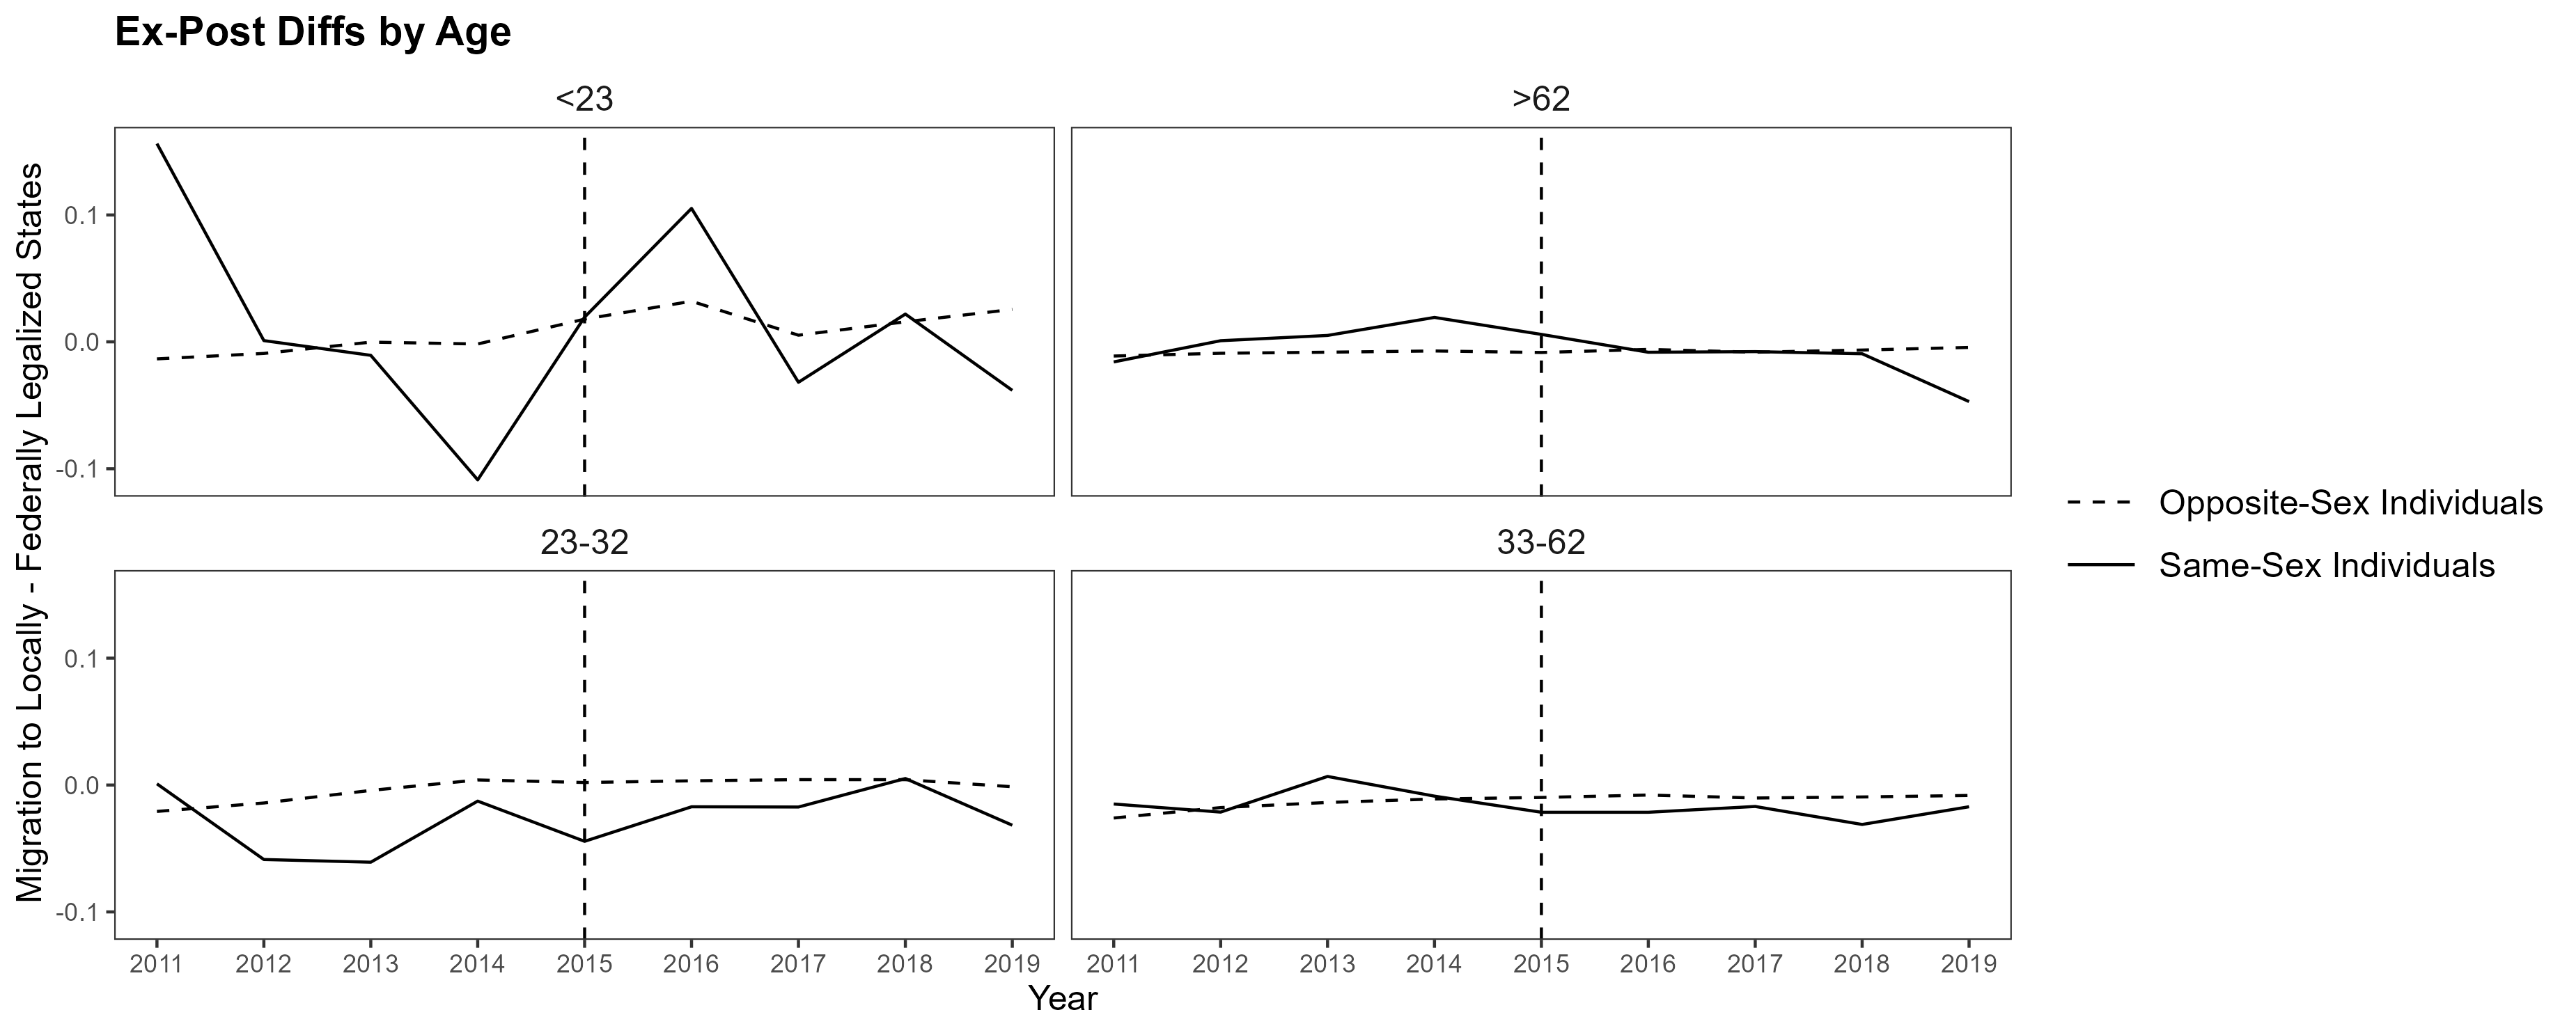
\includegraphics[width=0.75\linewidth]{outputs/summary_stats/age_post_diffs.png}
    \caption{Enter Caption}
    \label{fig: fig:enter-label}
\end{figure}

\begin{figure}
    \centering
    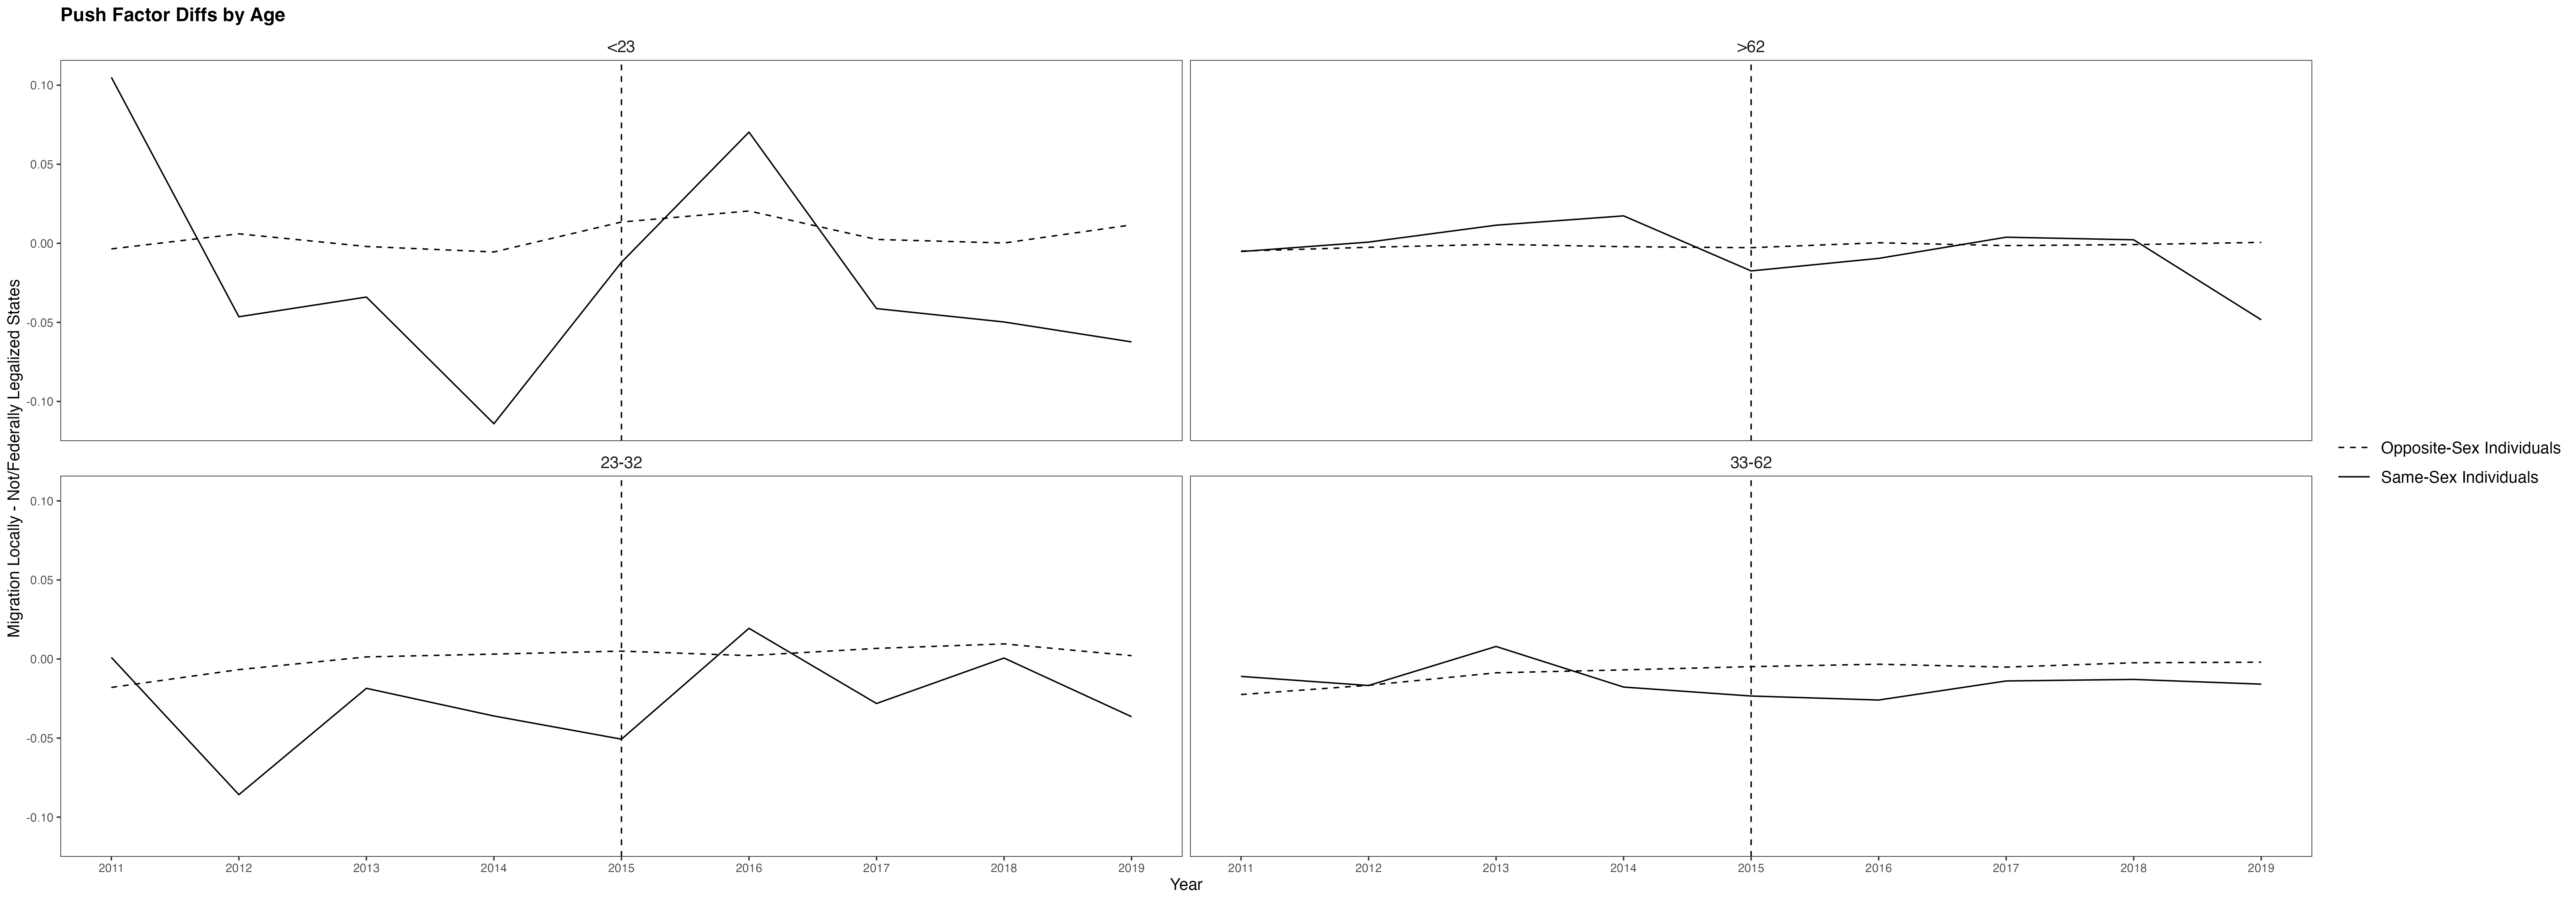
\includegraphics[width=0.75\linewidth]{outputs/summary_stats/age_ante_diffs.png}
    \caption{Enter Caption}
    \label{fig: fig:enter-label}
\end{figure}


%child
\begin{figure}
    \centering
    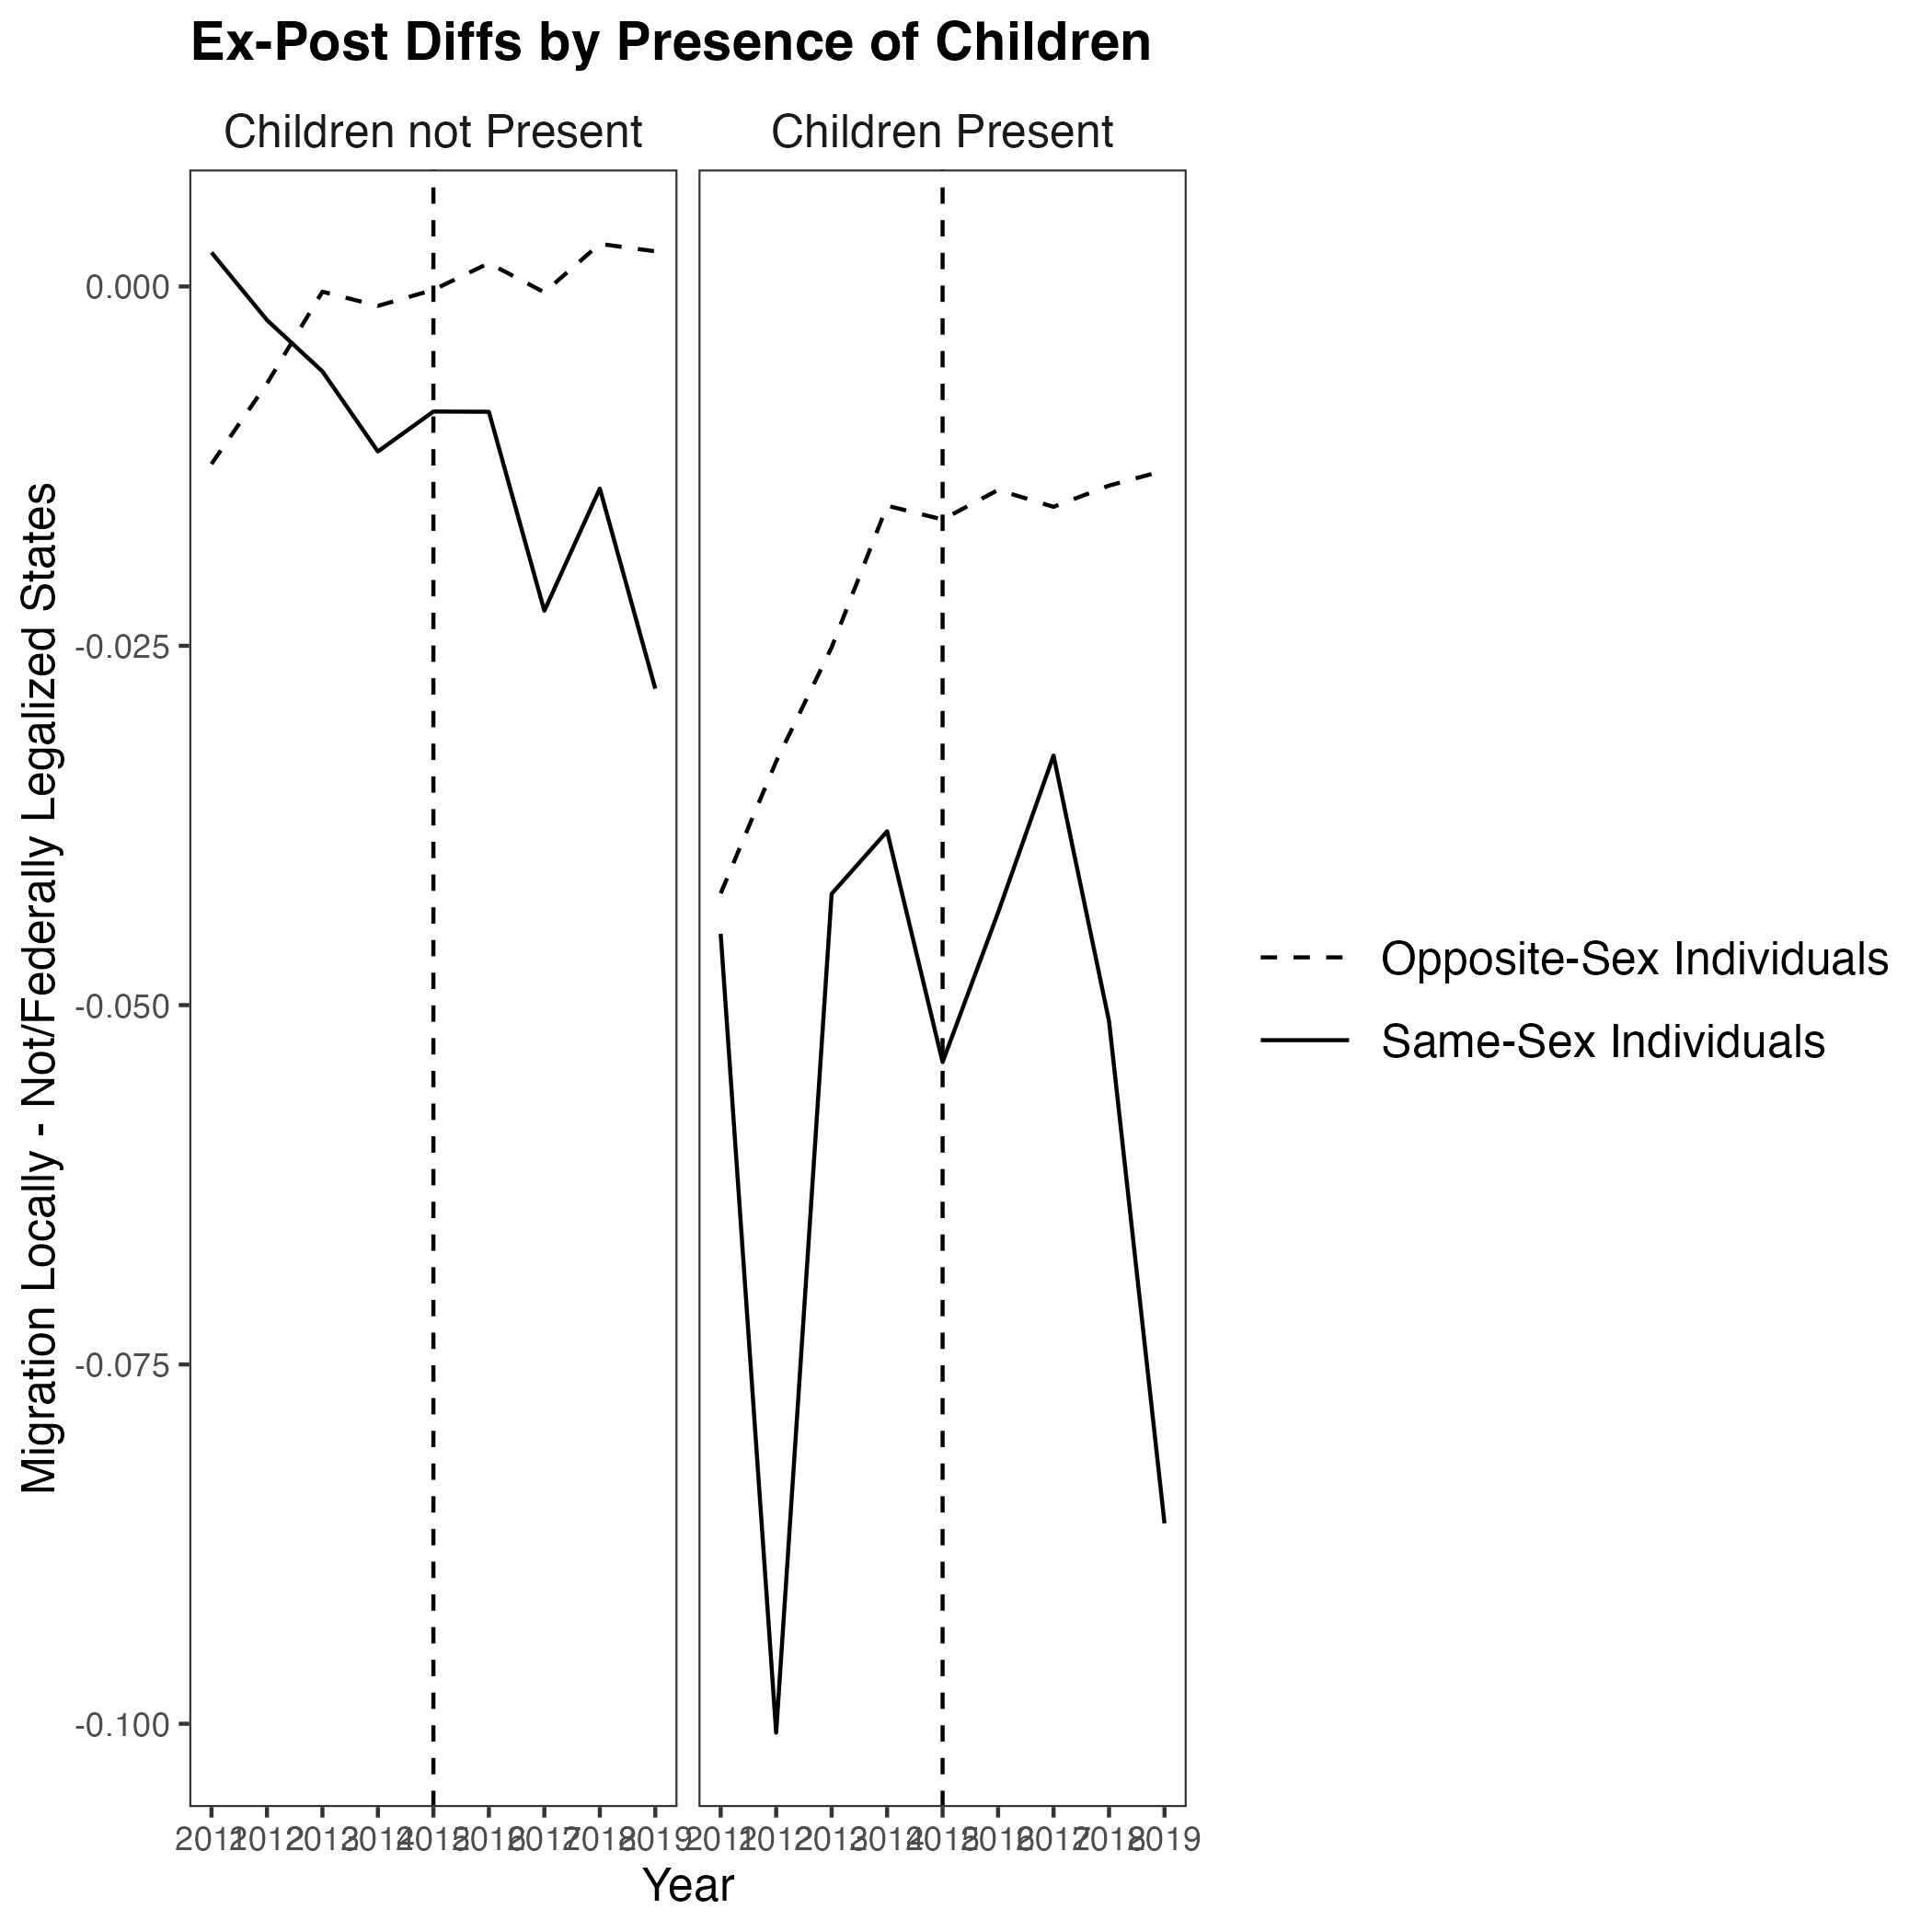
\includegraphics[width=0.75\linewidth]{outputs/summary_stats/child_post_diffs.png}
    \caption{Enter Caption}
    \label{fig: fig:enter-label}
\end{figure}

\begin{figure}
    \centering
    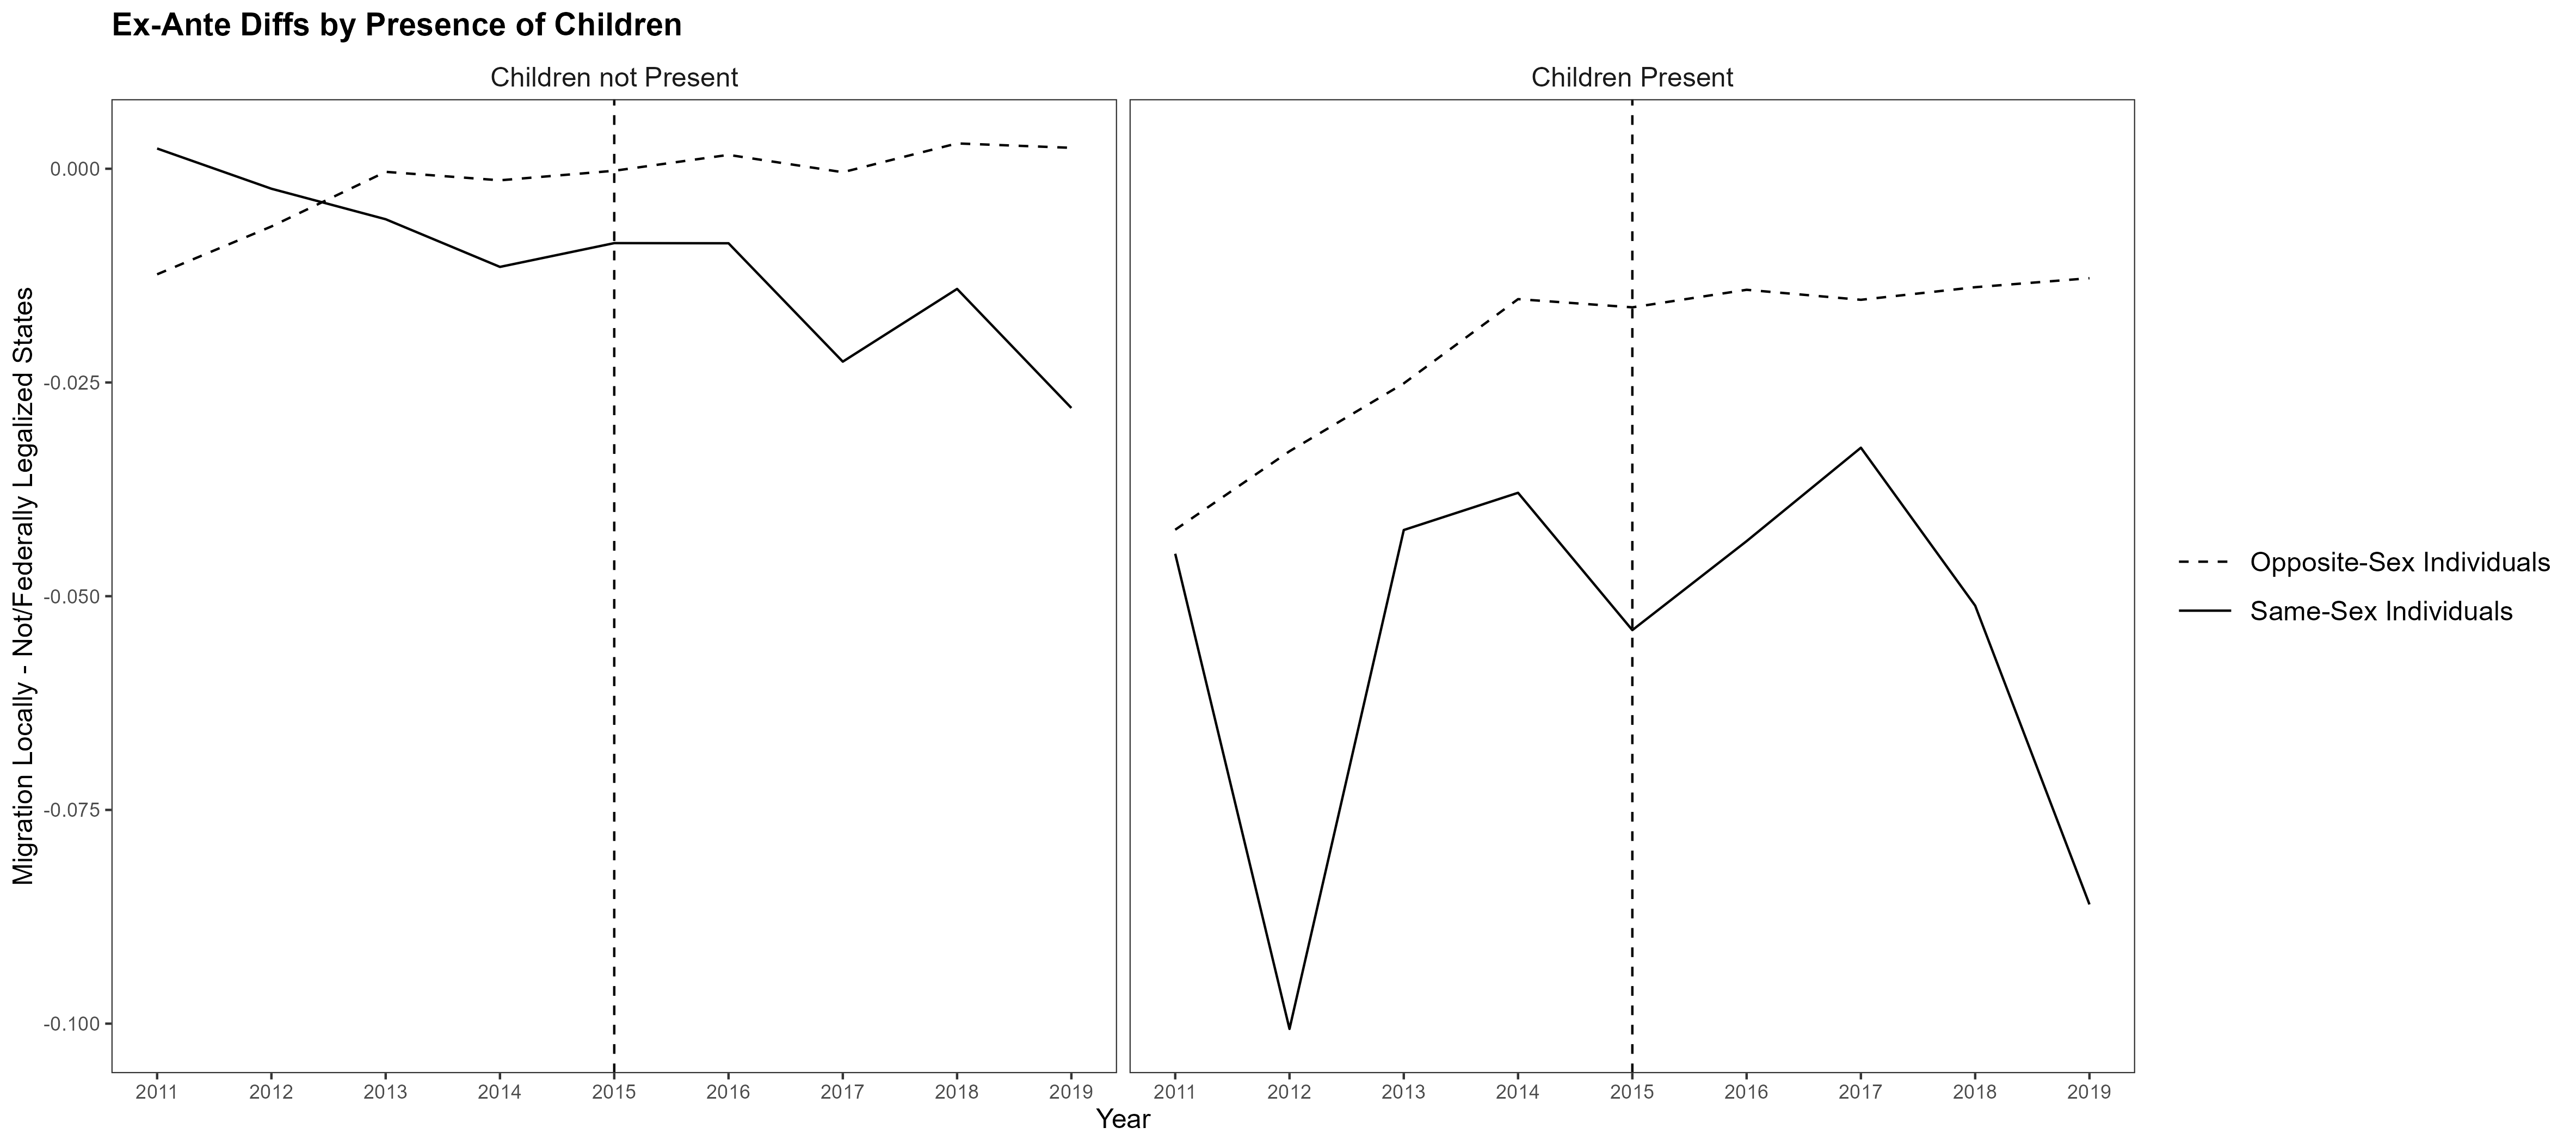
\includegraphics[width=0.75\linewidth]{outputs/summary_stats/child_ante_diffs.png}
    \caption{Enter Caption}
    \label{fig: fig:enter-label}
\end{figure}

%Education
\begin{figure}
    \centering
    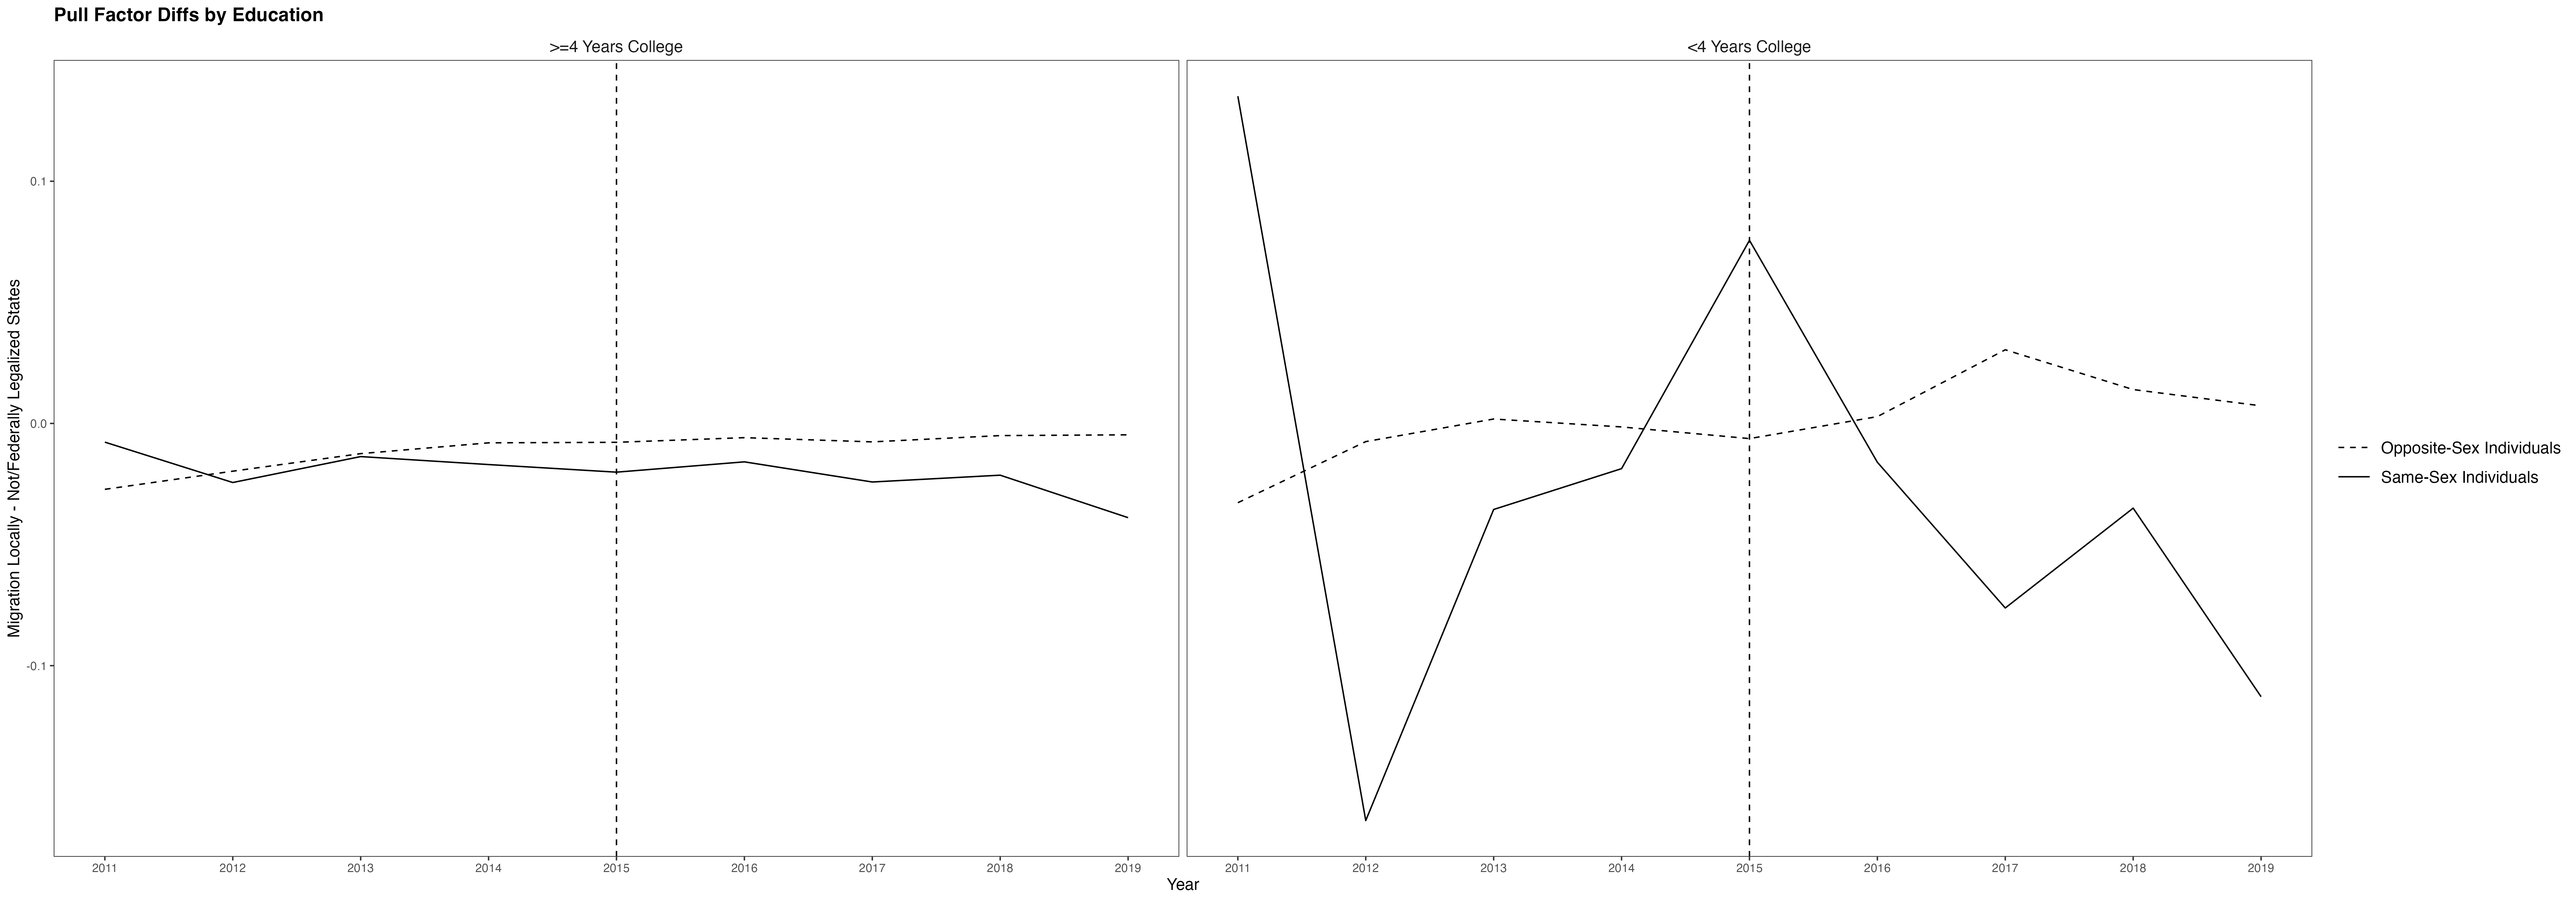
\includegraphics[width=0.75\linewidth]{outputs/summary_stats/educ_post_diffs.png}
    \caption{Enter Caption}
    \label{fig: fig:enter-label}
\end{figure}

\begin{figure}
    \centering
    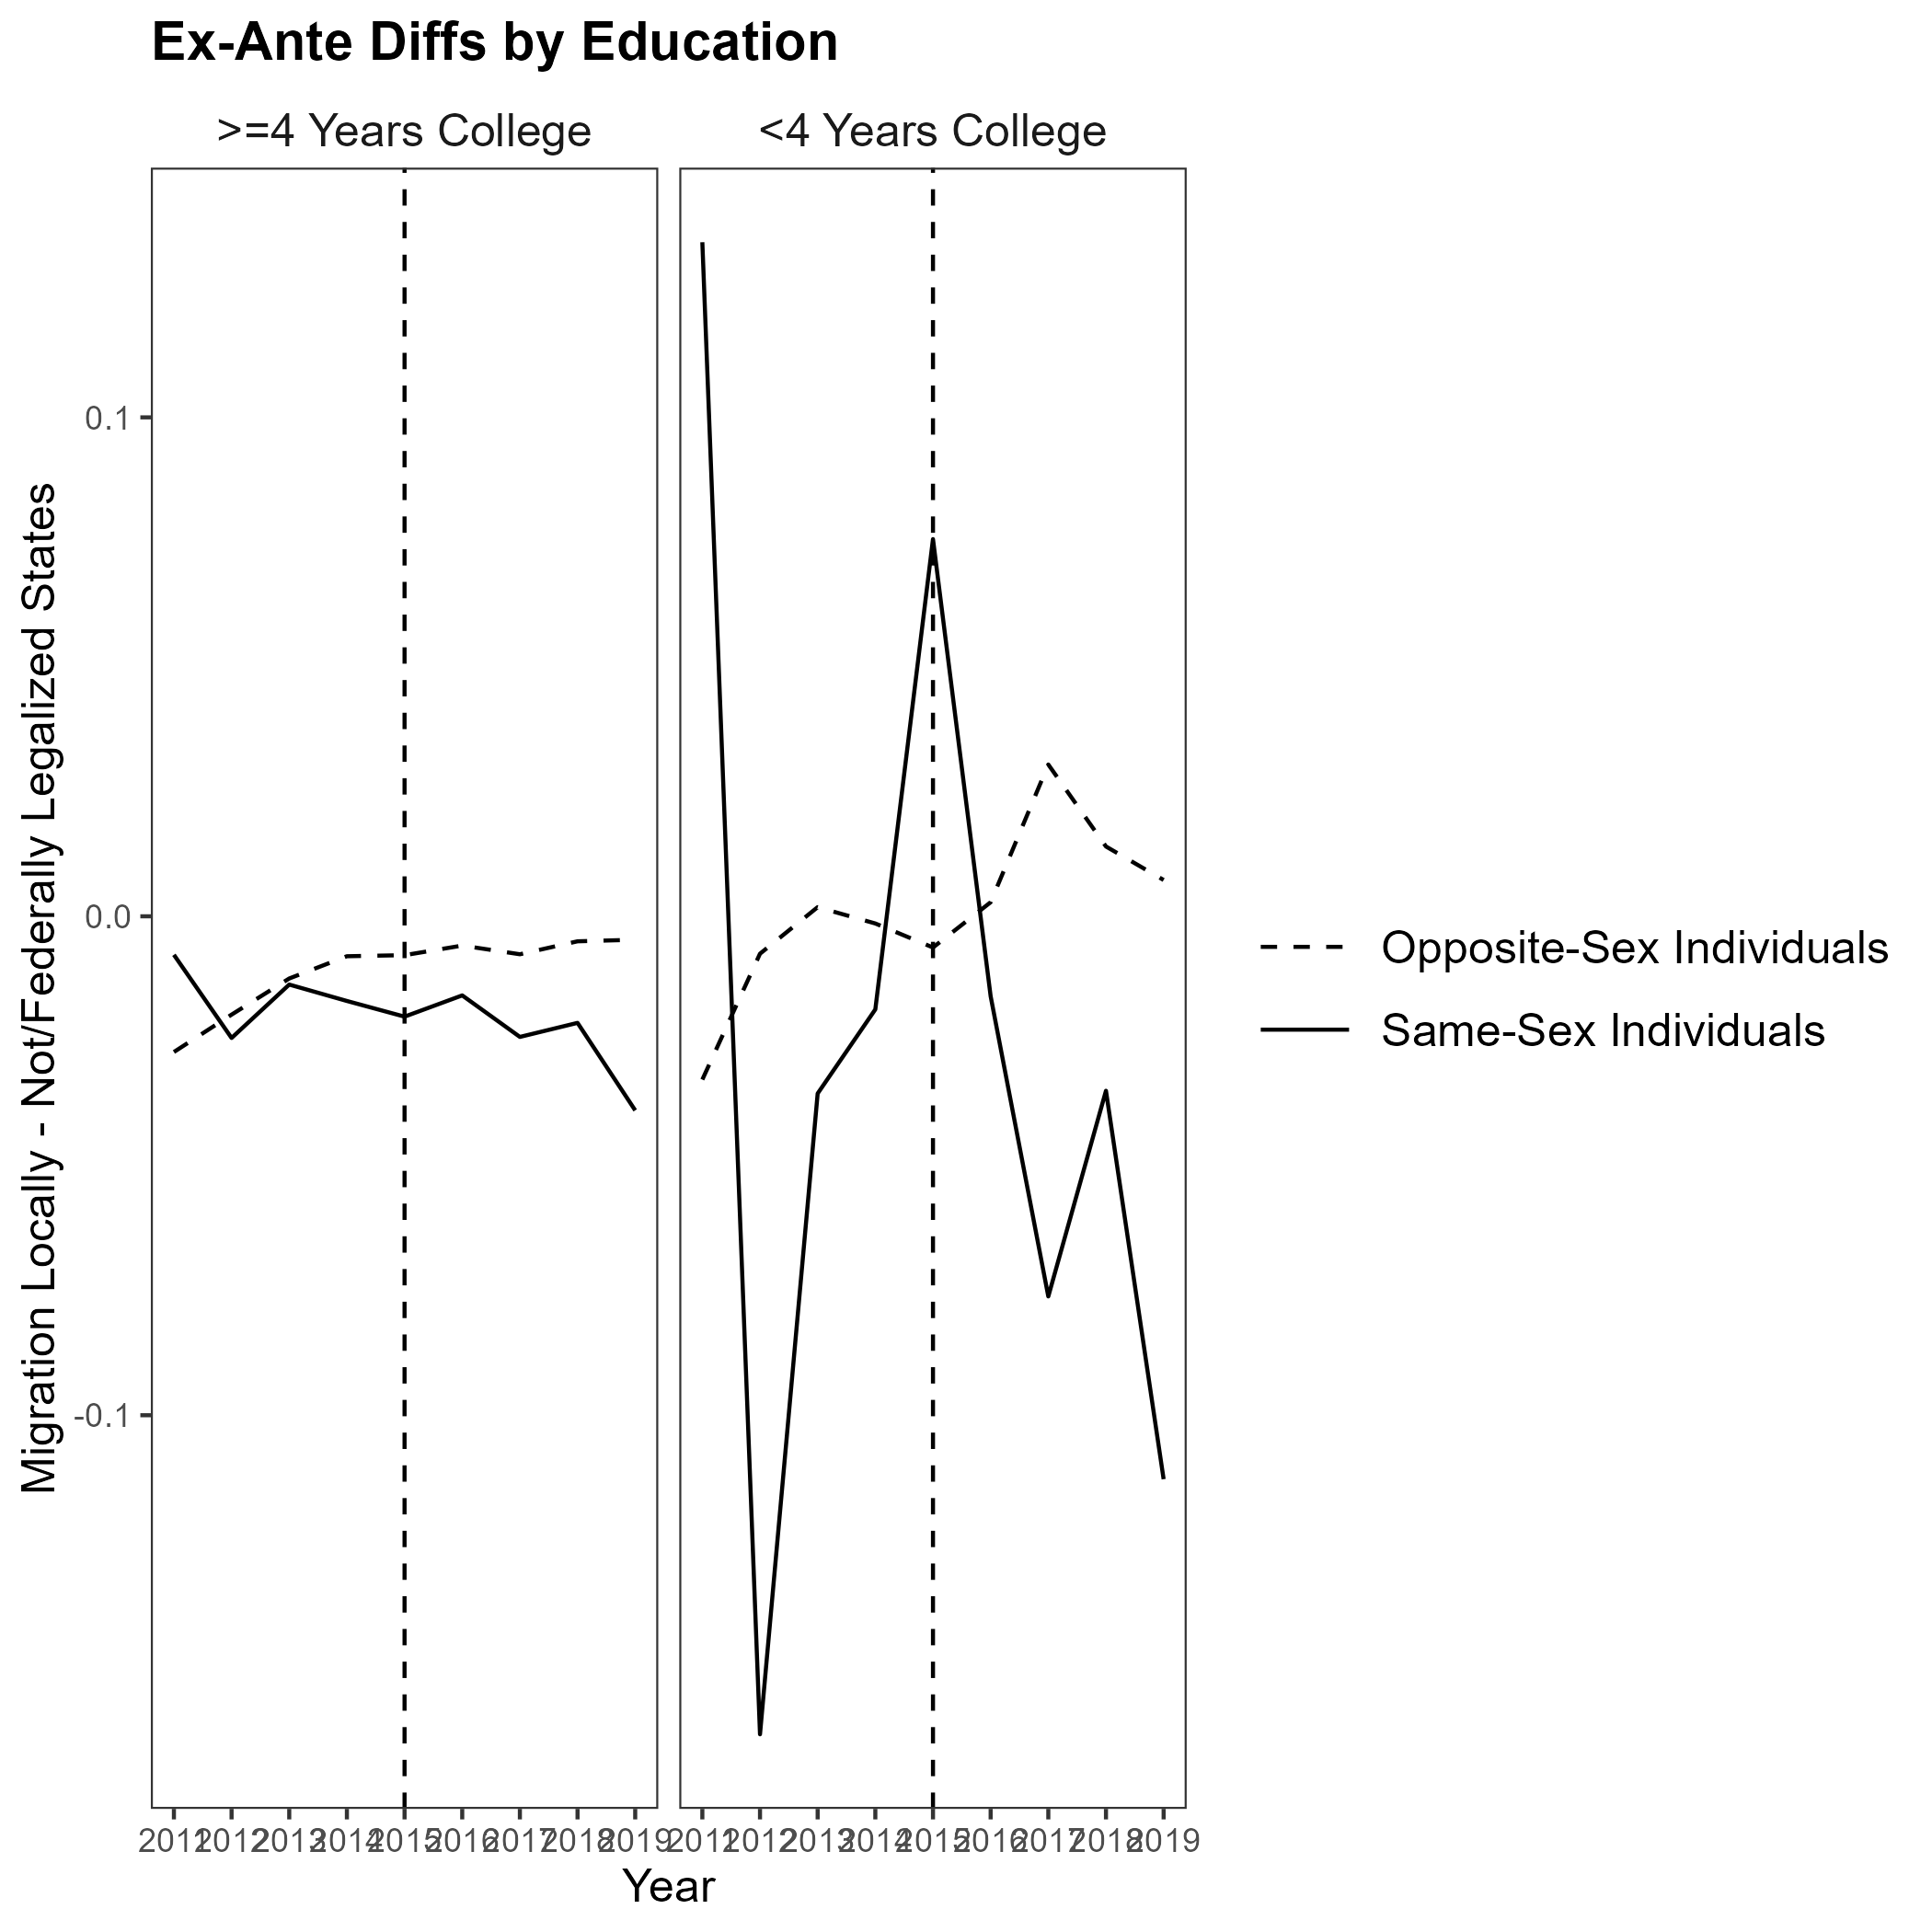
\includegraphics[width=0.75\linewidth]{outputs/summary_stats/educ_ante_diffs.png}
    \caption{Enter Caption}
    \label{fig: fig:enter-label}
\end{figure}

%income
\begin{figure}
    \centering
    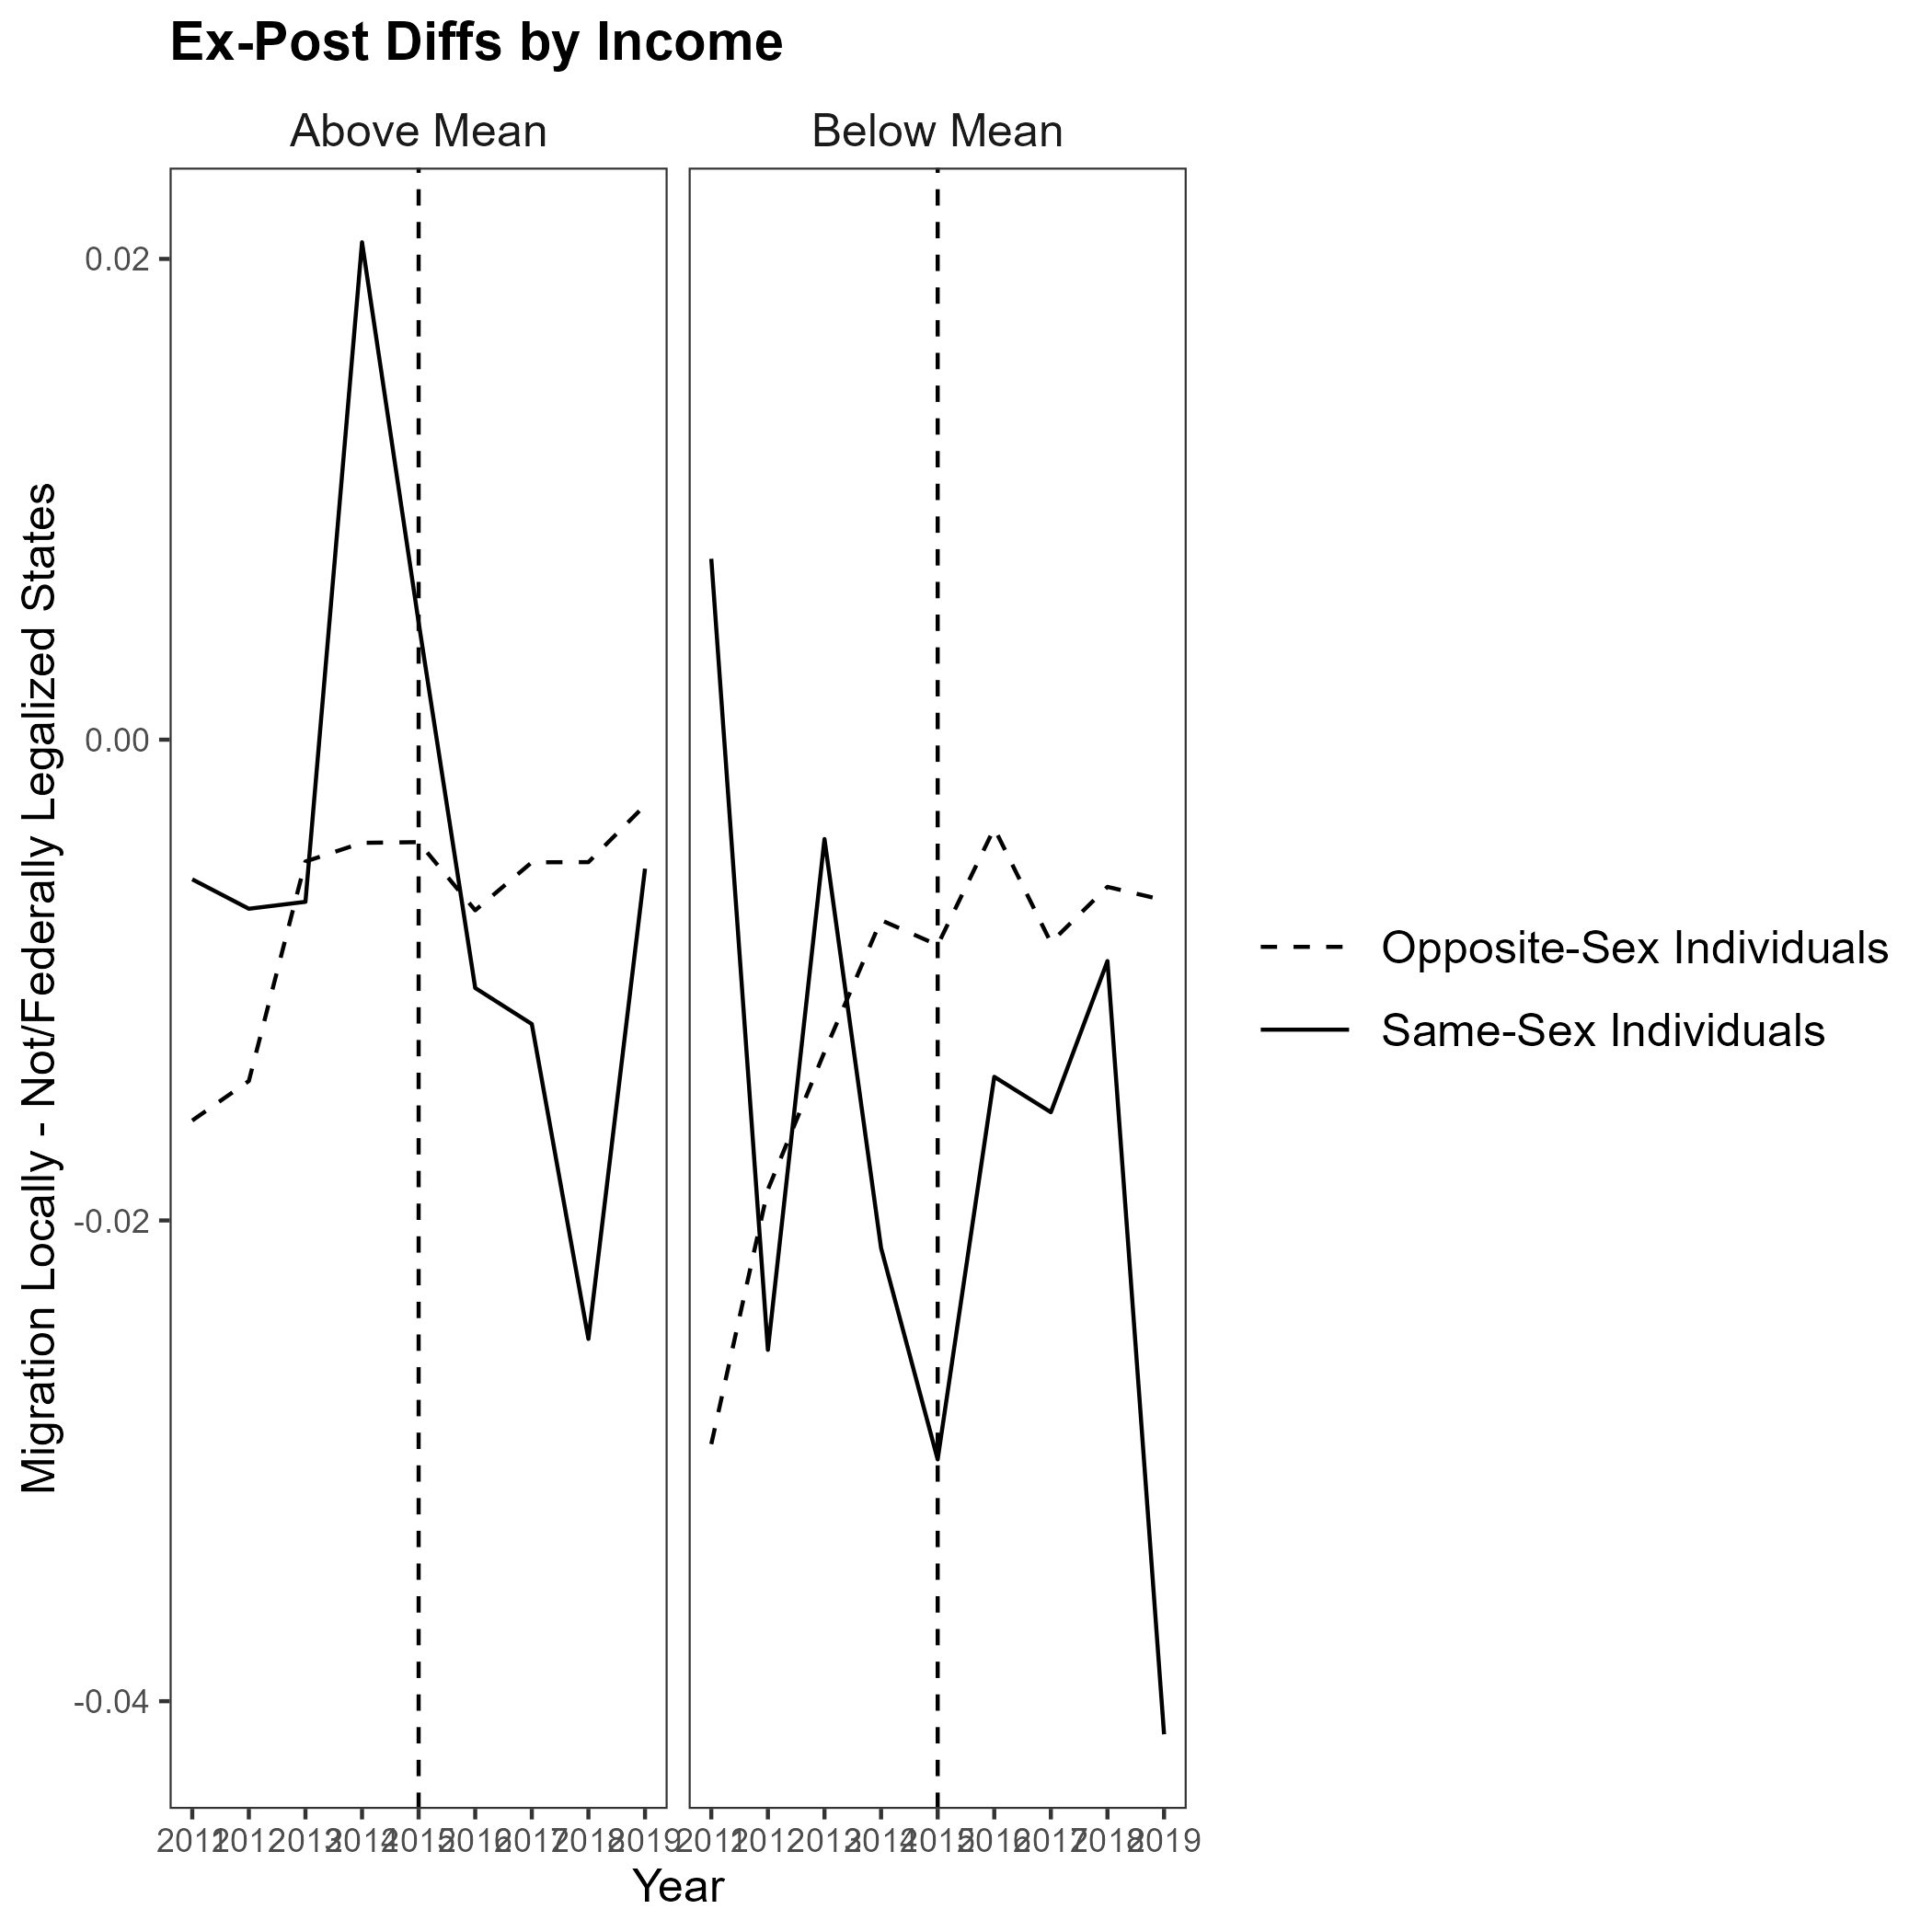
\includegraphics[width=0.75\linewidth]{outputs/summary_stats/inc_post_diffs.png}
    \caption{Enter Caption}
    \label{fig: fig:enter-label}
\end{figure}

\begin{figure}
    \centering
    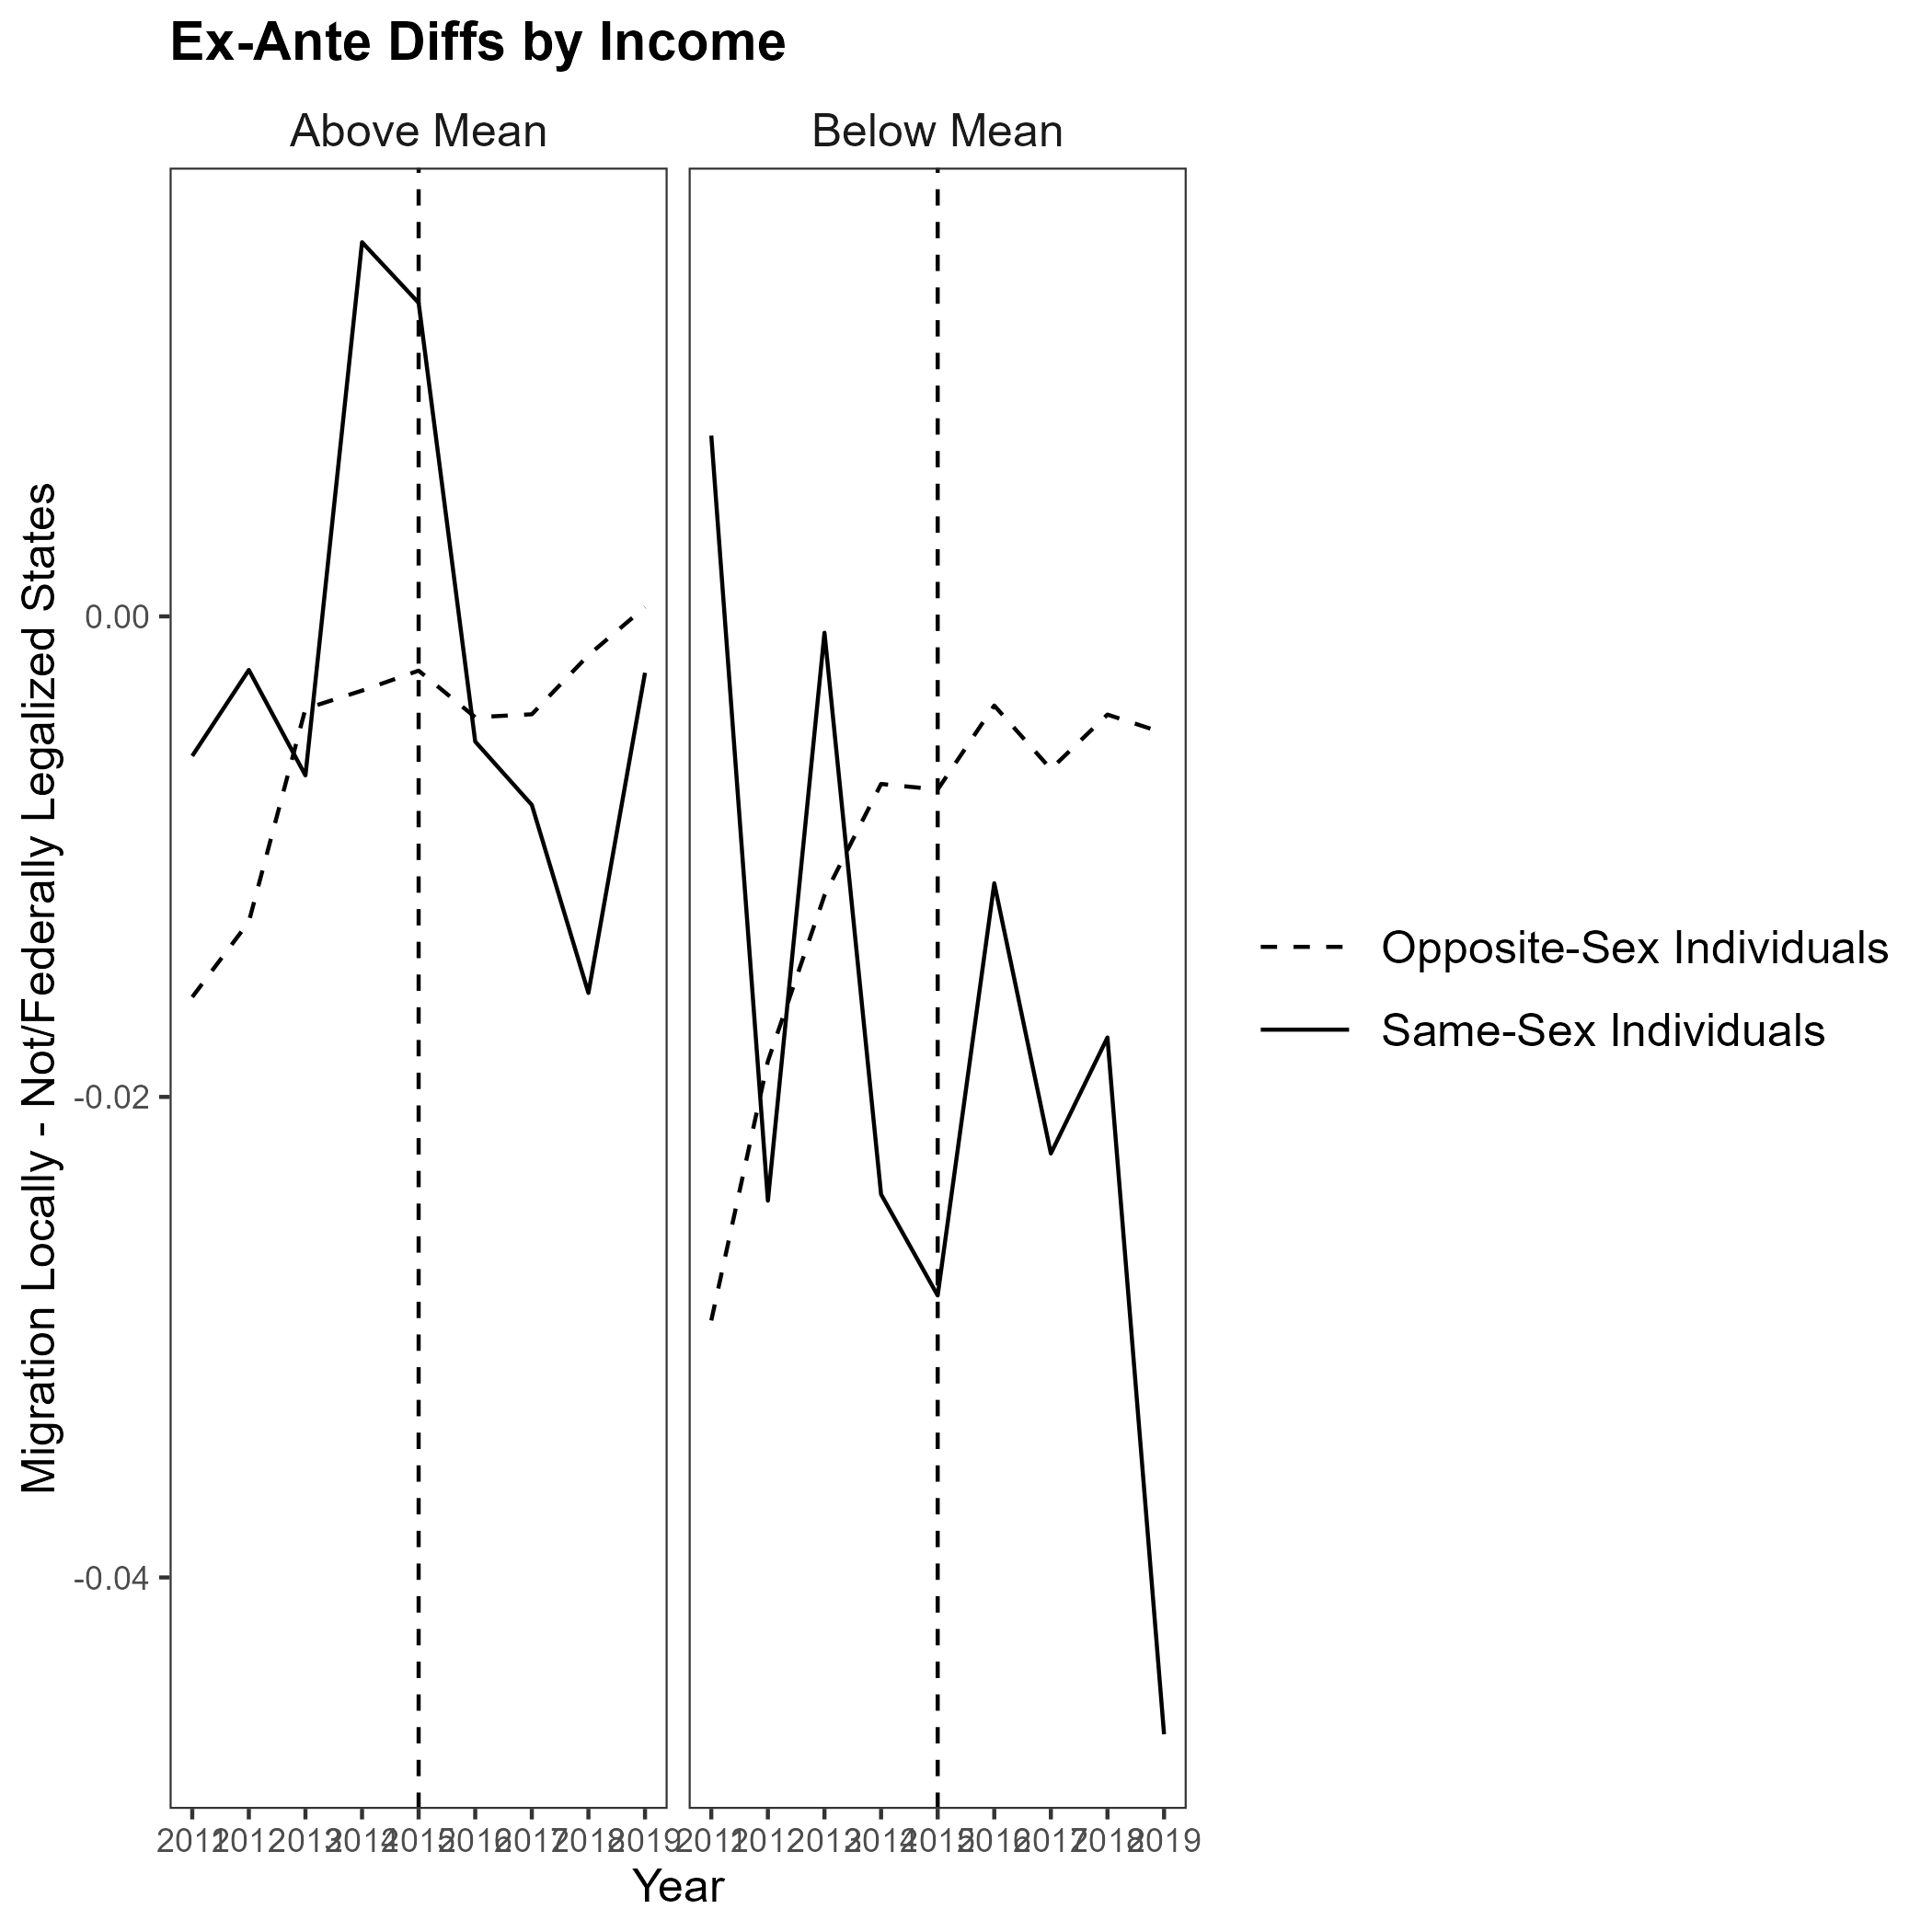
\includegraphics[width=0.75\linewidth]{outputs/summary_stats/inc_ante_diffs.png}
    \caption{Enter Caption}
    \label{fig: fig:enter-label}
\end{figure}

%MA
\begin{figure}
    \centering
    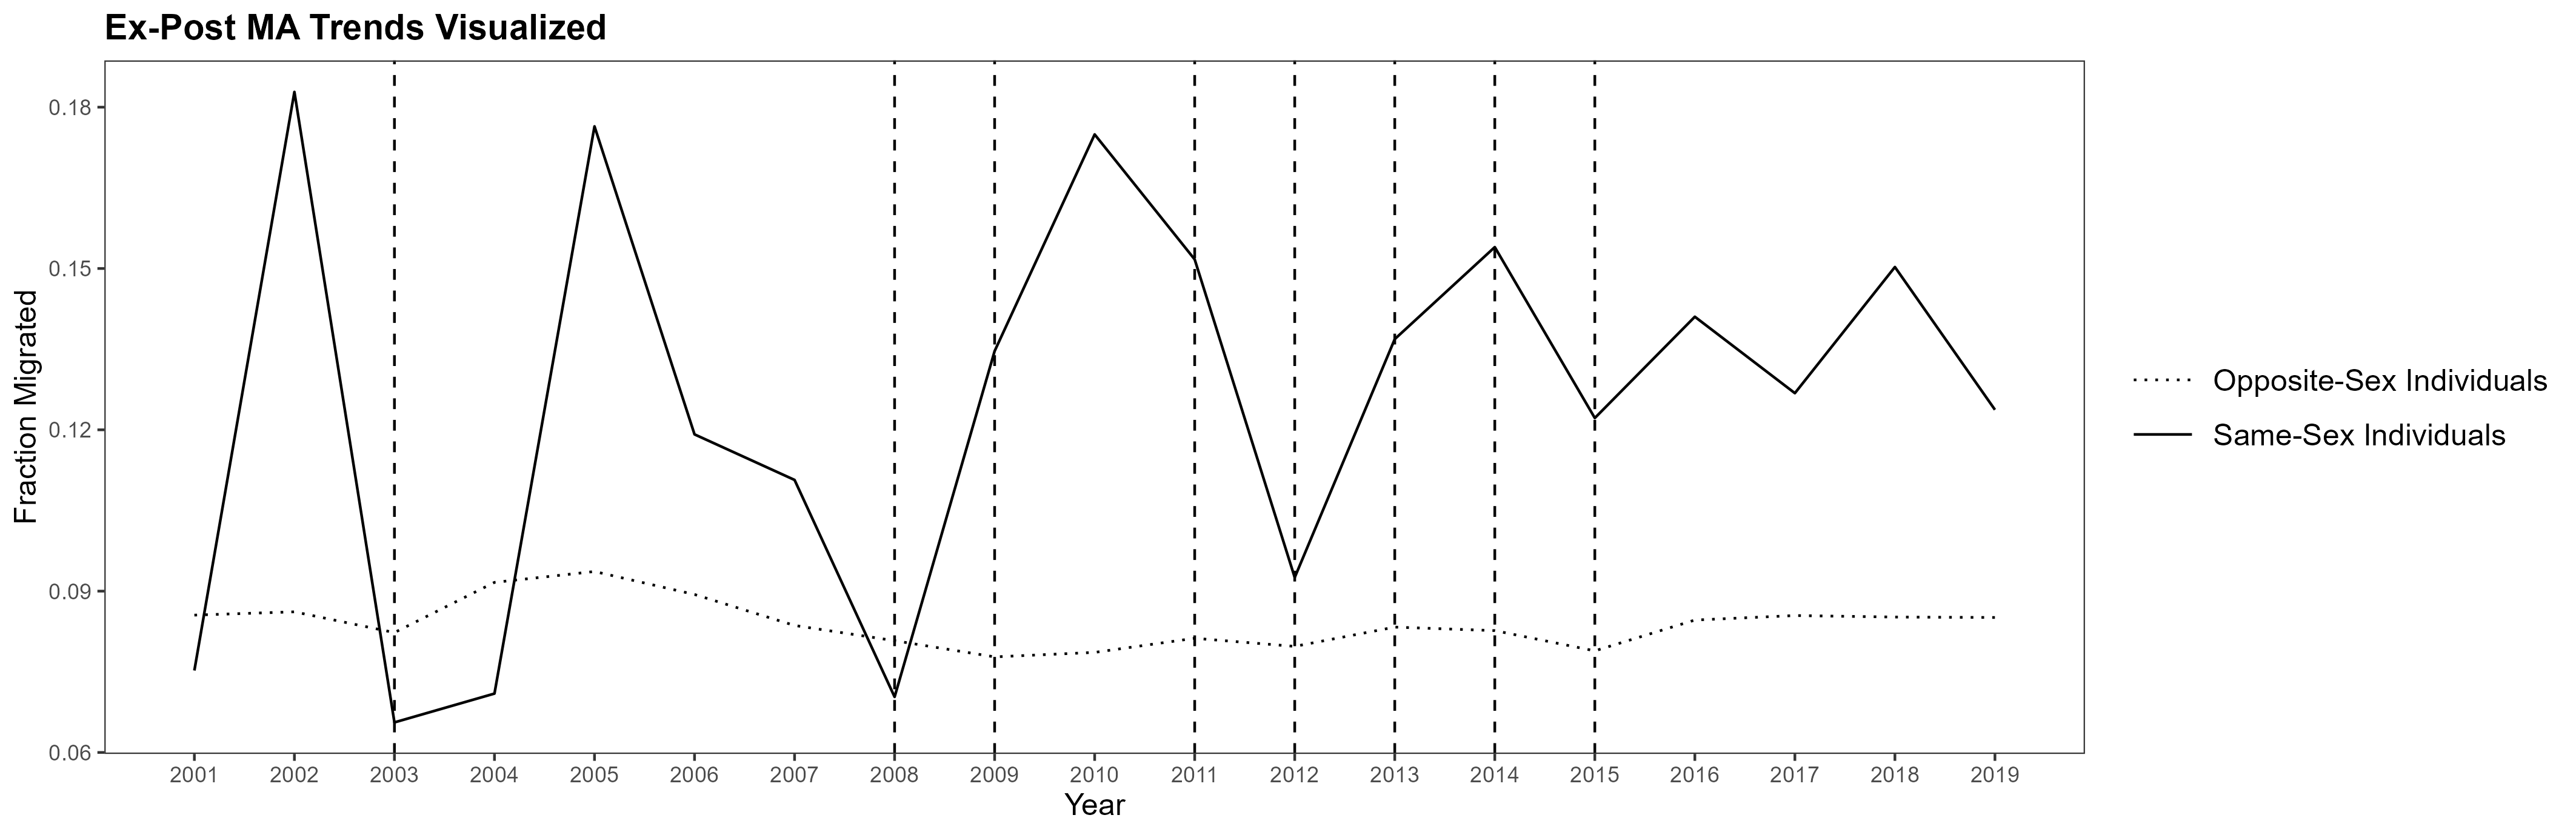
\includegraphics[width=0.75\linewidth]{outputs/summary_stats/MA_post_trends.png}
    \caption{Enter Caption}
    \label{fig: MA_post_trends}
\end{figure}

\begin{figure}
    \centering
    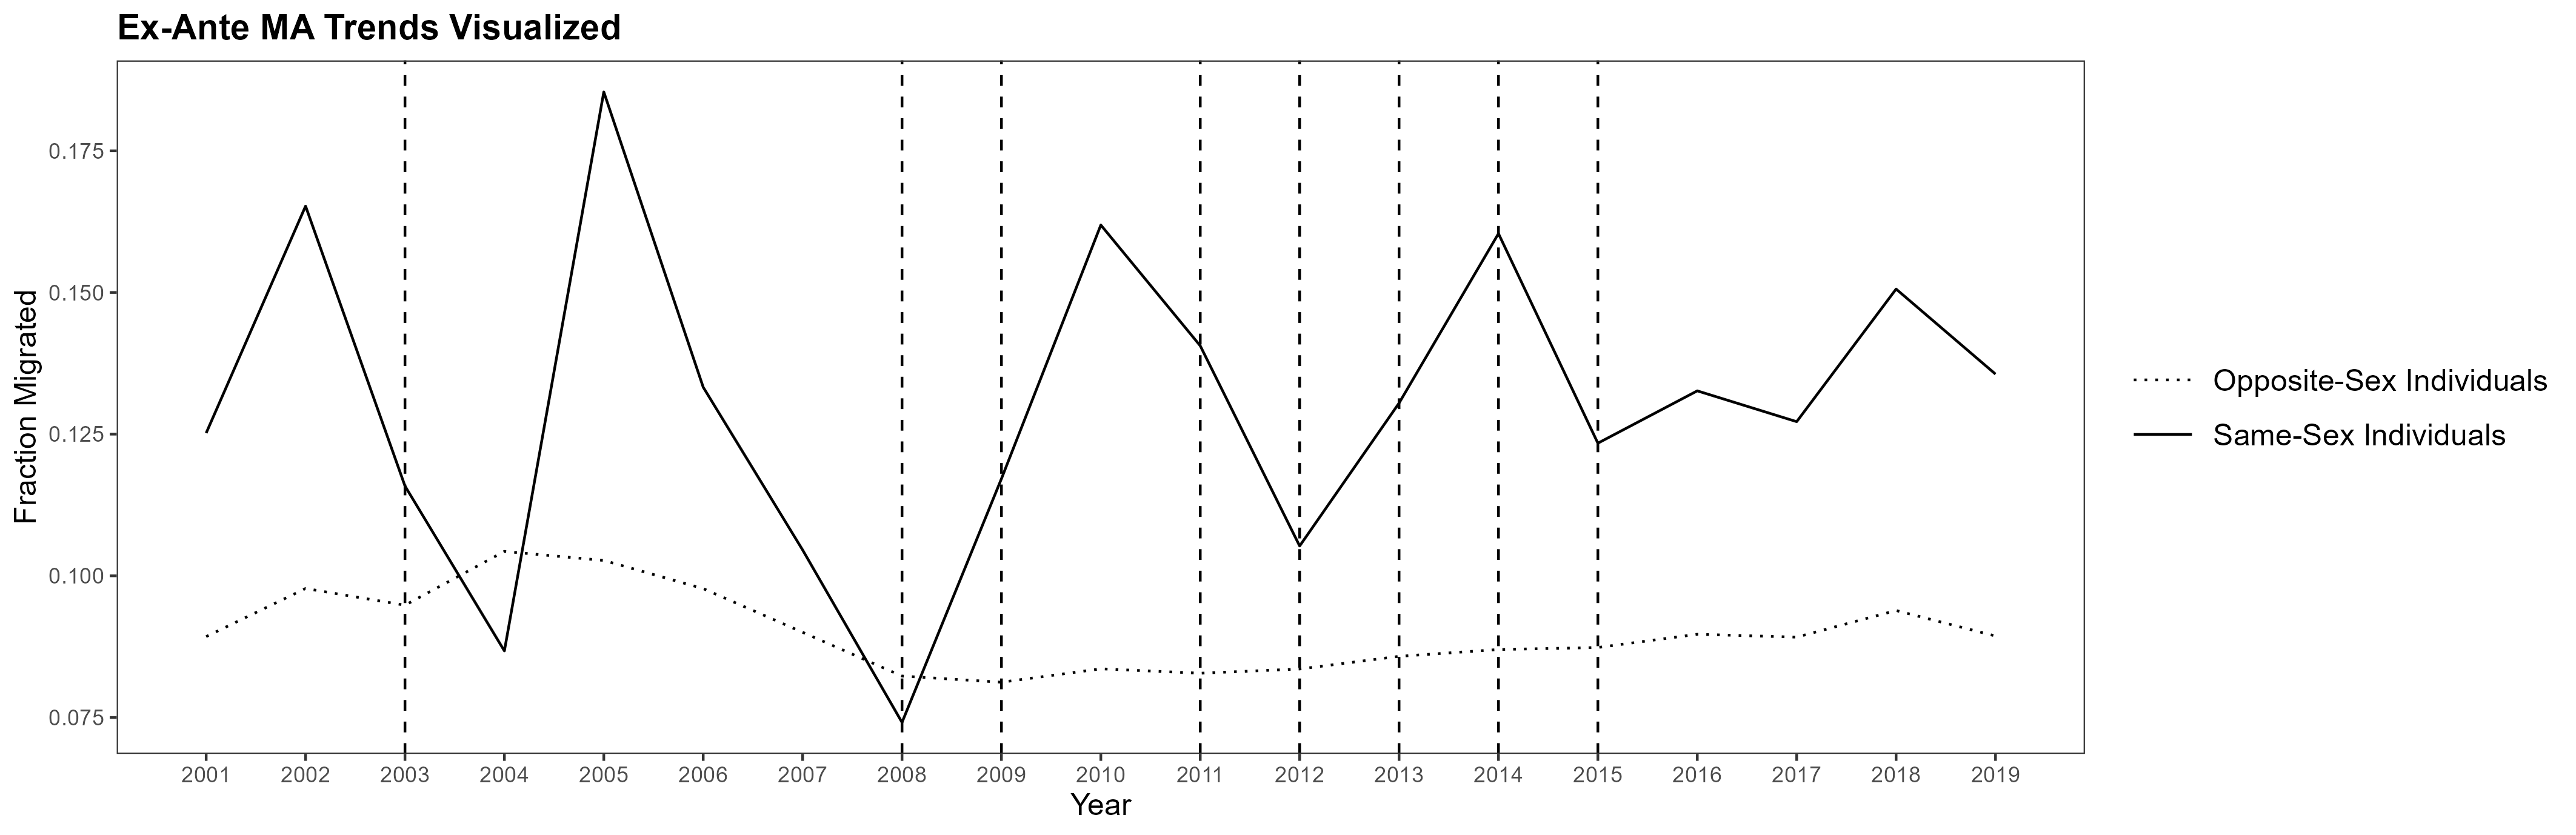
\includegraphics[width=0.75\linewidth]{outputs/summary_stats/MA_ante_trends.png}
    \caption{Enter Caption}
    \label{fig: MA_ante_trends}
\end{figure}

\end{document}